\documentclass[11pt,a4paper]{article}
\usepackage[margin=25mm]{geometry}
\usepackage[T1]{fontenc}
\usepackage[utf8]{inputenc}
\usepackage{lmodern,amsmath,amssymb,booktabs,longtable,array,graphicx,calc}
\usepackage{ragged2e}
\usepackage{needspace}
\usepackage{float}
\raggedbottom
% Float discipline. The panel figures are about 0.43\textheight each, so the
% default allowance of several top floats lets two of them plus a long-captioned
% table exceed the page and produce an overfull vbox in the output routine.
\setcounter{topnumber}{1}
\setcounter{bottomnumber}{1}
\setcounter{totalnumber}{2}
\renewcommand{\topfraction}{0.6}
\renewcommand{\bottomfraction}{0.4}
\renewcommand{\textfraction}{0.12}
\renewcommand{\floatpagefraction}{0.7}
\usepackage{xurl}
\usepackage[round]{natbib}
\usepackage[colorlinks=true,allcolors=blue]{hyperref}
\usepackage{bookmark}
\usepackage{caption}
\captionsetup{font=small,labelfont=bf}
\setlength{\emergencystretch}{3em}
\providecommand{\tightlist}{\setlength{\itemsep}{0pt}\setlength{\parskip}{0pt}}
\providecommand{\pandocbounded}[1]{#1}
\title{Unequal Job Opportunities and Well-Being Inequality: A Latent-Jobs Structural Decomposition}
\author{Hisham Haydar\\University of Luxembourg and LISER}
\date{Build: 10 September 2026\\Discussion draft}
\begin{document}
\maketitle
\begin{abstract}
We study how unequal job opportunities contribute to inequality in money-metric well-being. Our normative reference retains each household's own preferences and its own set of reachable jobs, while assigning the same disposable-consumption level to every job in that reference set; the money metric is the level at which the household's ex-ante evaluation of the reference matches the evaluation of the prospect it actually faces. We model labour supply as a choice among latent jobs and estimate preferences, job access and earning opportunities jointly on French EU-SILC data, with EUROMOD computing taxes, benefits and disposable income at every alternative work arrangement. We then introduce and implement a structural decomposition of the resulting inequality: well-being is recomputed under counterfactual equalizations of preferences, job access, earning opportunities, and household resources and needs, and the interactions among them are allocated with a grouped Shapley--Owen--Shorrocks rule. In the baseline Gini decomposition, labour-market opportunities account for 55.9 per cent of well-being inequality among single-adult households, of which job access alone carries 49.2 per cent, against 9.9 per cent for preferences and 34.2 per cent for household resources and needs. Among couples the balance differs: earning opportunities and resources and needs account for 35.7 and 51.2 per cent, while job access accounts for 8.2 and preferences for 4.8. Access exceeds earning opportunities for single adults, and the ordering reverses for couples, under all six inequality indices we report; the sign of the single-adult preference contribution is not robust across indices.
\end{abstract}

\emph{Preliminary results. Intervals on the headline shares are cluster-robust parameter percentiles from 100 draws and are reported separately from the integration band, never merged with it. The subdivision of couples resources against household composition rests on a repricing completed after this draft was planned; the joint contribution remains the headline component and the subdivision is reported beside it.}

\section{Introduction}\label{introduction}

Two people can work the same hours for the same hourly pay and be very differently placed. One chose that job from several that were open; the other took the only offer available. Their earnings are identical and their circumstances are not. Income comparisons record the outcome and cannot separate the two cases, and the difference matters for how unequal we should judge well-being to be.

The same ambiguity runs through the whole distribution. Low earnings can describe someone who values leisure highly and chose short hours, someone who cannot obtain a well-paid job, or someone whose family resources make a different work choice affordable. These are observationally entangled and economically different. A distribution of income is a distribution of outcomes with the explanations already mixed in.

The ambiguity matters for measurement, not only for interpretation. If we want to know how much of the inequality we observe is associated with unequal access to employment, hours arrangements and wage offers, we need two things that an income distribution does not supply. We need a behavioural model that separates what a household wanted from what it could reach, and we need a rule for comparing people whose opportunities and whose tastes both differ. Neither is optional: without the first there is nothing to attribute, and without the second there is no defensible way to say who is better off.

\textbf{The normative reference.} Comparing well-being when individuals face different job opportunities requires a reference that specifies how those opportunities enter the comparison. We draw on the own-set equal-consumption criterion of Haydar and Maniquet (2026), work in progress. In its deterministic formulation, the criterion assigns to an attained situation the consumption level that would make the individual's preferred job within their own ability set equally good, when every feasible job provides that same consumption. The reference therefore retains the individual's own opportunities and own preferences while removing variation in pay from the reference bundles. Writing \(A_i\) for the jobs available to \(i\) and \(z_i\) for the attained situation, the reference level solves

\[u_i(z_i)=\max_{j\in A_i}\,u_i(W_i,j).\]

The argument being solved for is an amount of consumption, so the measure is money-metric by construction; there is no second conversion from an index into euros.

\begin{figure}[H]
\centering
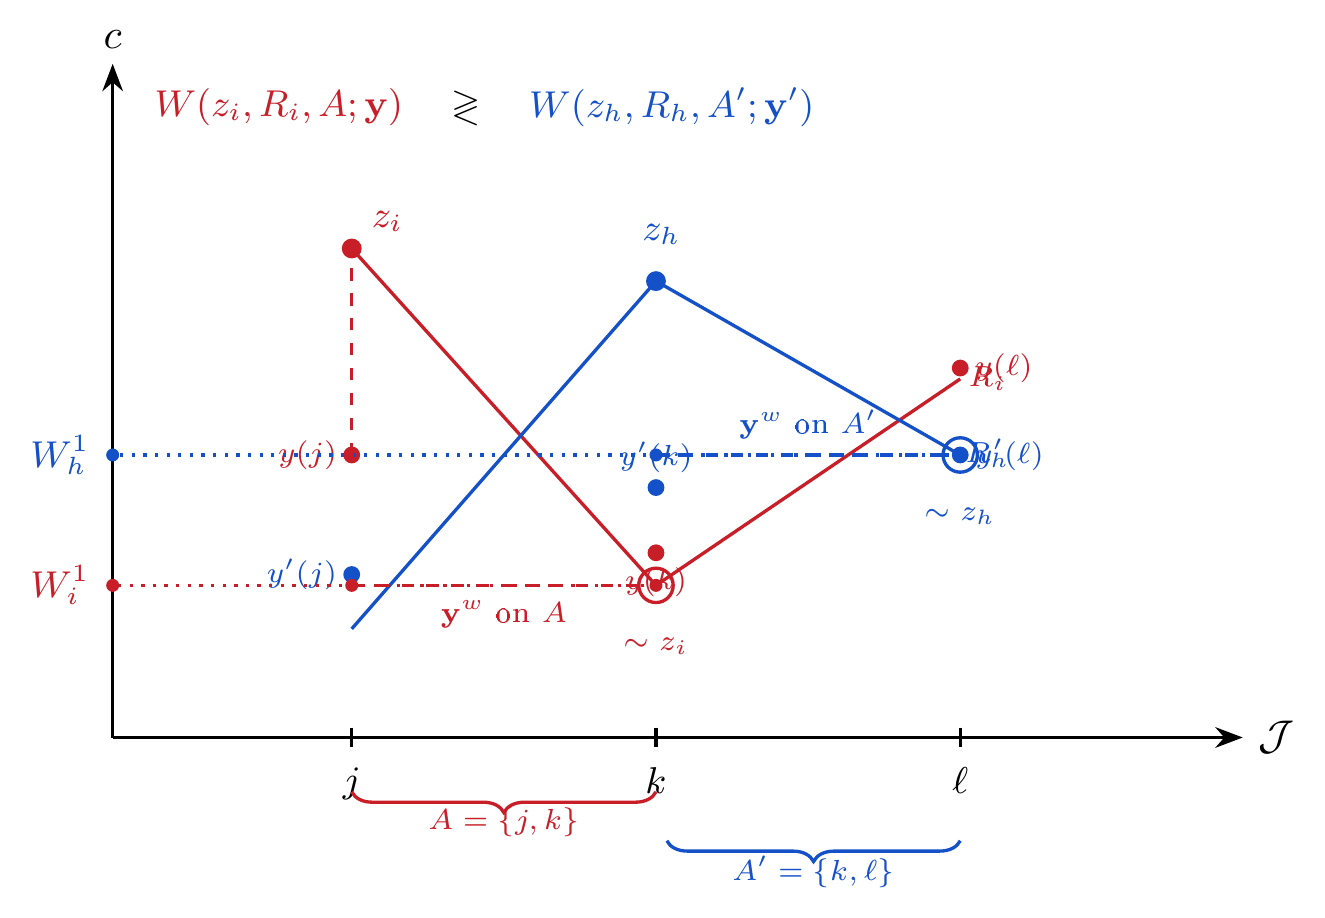
\includegraphics[width=0.95\linewidth,height=\textheight,keepaspectratio,alt={Own-set equal-consumption equivalents. Individuals with preferences R\_i,R\_h and ability sets A=\textbackslash\{j,k\textbackslash\} and A\^{}\{\textbackslash prime\}=\textbackslash\{k,\textbackslash ell\textbackslash\} attain z\_i and z\_h. For each individual, a common consumption level is assigned to every job in their own set; the level at which the preferred reference job becomes indifferent to the attained bundle is the money metric. Adapted from Haydar and Maniquet (2026), work in progress. This is the deterministic construction; the estimated measure is its ex-ante extension, defined in Section 4.}]{figures/v5/theory_w1.png}
\caption{\textbf{Own-set equal-consumption equivalents.} Individuals with preferences \(R_i,R_h\) and ability sets \(A=\{j,k\}\) and \(A^{\prime}=\{k,\ell\}\) attain \(z_i\) and \(z_h\). For each individual, a common consumption level is assigned to every job in their own set; the level at which the preferred reference job becomes indifferent to the attained bundle is the money metric. Adapted from Haydar and Maniquet (2026), work in progress. This is the deterministic construction; the estimated measure is its ex-ante extension, defined in Section 4.}
\end{figure}

We adapt this principle to an estimated distribution of latent jobs. The empirical object is not the deterministic maximum but its ex-ante counterpart: the household's evaluation of the reference prospect, integrated over the jobs it may reach, is set equal to its evaluation of the prospect it actually faces. Section 4 states the stochastic formulation, derives its closed form, and says precisely which properties of the deterministic criterion carry over and which are not claimed.

One comparative static is worth stating plainly at the outset, because it is easy to misread. Holding the attained situation fixed, a person with a larger reference menu may need less uniform consumption to reach the same satisfaction. When actual opportunities change, however, both the attainment and the reference menu change. The net effect on equivalent consumption depends on both. Measuring attainment against one's own opportunities is therefore not a claim that larger menus are intrinsically better, and we make no such claim.

\textbf{The empirical approach.} The behavioural half is a random-utility, random-opportunity model of job choice. A job is a package: an employment state, an occupation, a weekly hours arrangement and an hourly wage. Households rank packages by consumption and leisure, and the packages differ in how available they are. Both the preferences and the household-specific intensity of availability enter one likelihood and are estimated jointly; neither is observed as a complete schedule. Every package is priced through the French tax-benefit system, so a change of hours or occupation moves disposable income through the actual schedule of taxes and transfers rather than a linear approximation. We estimate the model separately on 1,540 single-adult and 2,223 couple households drawn from French EU-SILC, with couples choosing jointly under a shared household budget.

The normative half then yields, for each household, an equivalent flat consumption level. To decompose its inequality we do not linearise. We define four structural equalization operators, one for preferences, one for job access, one for earning opportunities and one for household resources and needs; we recompute every household's welfare level, and the inequality of the resulting distribution, under each of the sixteen coalitions of those operators; and we allocate the interactions among them with the grouped Shapley--Owen--Shorrocks rule. The allocation is exhaustive by construction and the closure is verified numerically rather than imposed.

\textbf{What we find.} Among single-adult households, labour-market opportunities carry 55.92 per cent of the inequality in the money metric, of which job access alone carries 49.16 per cent and earning opportunities 6.76. Preferences carry 9.88 per cent and household resources and needs 34.20. Among couples the composition is different rather than the total: earning opportunities carry 35.72 per cent and resources and needs 51.20, while job access carries only 8.23 and preferences 4.85. Single adults are access-dominated on the labour-market side and couples are earnings- and resource-dominated. We report that contrast as a finding and do not attach a mechanism to it.

Two qualifications belong with the headline. First, the ordering of access against earning opportunities is the robust part: access exceeds earning opportunities for single adults under all six inequality indices we report, and the ordering reverses for couples under all six. The complete ordering of all four components is not robust in that sense, and the sign of the single-adult preference contribution changes outside the Gini. Second, an allocated share is an average of marginal contributions over coalition orders. It is not the reduction that equalizing that group alone would achieve. For single adults the two differ instructively: equalizing preferences alone would \emph{raise} the Gini by 13.0 per cent, while the allocated preference share is a positive 9.88 per cent. Section 5 explains why both statements are correct.

\textbf{Relation to existing work.} Every ingredient here has antecedents, and the contribution is the combination and the empirical answer, not any one step.

Modelling labour supply as choice among latent jobs, with preferences and offer intensities identified jointly from one likelihood, is due to \citet{aaberge1995} and \citet{aaberge1999}, developed by \citet{dagsvikstrom2006} and \citet{dagsvikjia2016}, surveyed by \citet{aaberge2018}, and set out for applied work by \citet{capeau2016}. We inherit that framework, including its distinction between the intensity of an offer and the probability of a choice, and its reliance on excluded opportunity shifters to separate components that choices alone identify only jointly. \citet{capeau2016} also supply two of the identifying restrictions we maintain: the wage-offer distribution is independent of offered hours, and a local unemployment measure shifts availability while being excluded from preferences. Their Belgian application already covers single women, single men and couples, so covering both household types is not itself a contribution.

Combining such a model with a monetary welfare evaluation is also established. \citet{aaberge1995} translate attained utility into an equivalent income against a stated reference household, choice set and tax system, and \citet{aaberge2004} evaluate reforms with joint household choice and restricted hours. \citet{jiathoresen2021} make the case for the job-choice model in exactly this role and report a distribution of compensating variation for a Norwegian reform, and \citet{jacquet2026} compare a standard compensating variation with one computed after replacing preference characteristics by reference values. All four evaluate a \emph{change} between policy regimes. Our object is a cross-sectional distribution of levels under one policy system, and its attribution. A reform gain and a level have different origins and different denominators; a small preference-related reform difference would not imply a small preference share in our decomposition, and our shares do not estimate their reform gains.

The normative half draws on the literature that refuses to resolve interpersonal comparison by assuming common preferences. \citet{fleurbaeymaniquet2006}, \citet{fleurbaeymaniquet2017} and \citet{fleurbaeymaniquet2018} set out how a reference bundle encodes a position on compensation and responsibility; \citet{decosterhaan2015} and \citet{bargain2013} show empirically how much a welfare ordering moves with that choice. Their references fix a wage or an unearned-income intercept and maximize over a deterministic budget set. Ours fixes consumption across the alternatives of an estimated opportunity distribution and integrates. That is a different reference and, as Section 6 records, the ordering is sensitive to it.

The closest decomposition precedents are two. \citet{muehlhan2023} combines a structural labour-supply model with involuntary-unemployment restrictions and a Shapley attribution, decomposing the change in German household \emph{income} inequality into temporal factors and binary restrictions. \citet{creedyherault2011}, in the section that constructs money-metric distributions under alternative policy and population states, decompose a change in inequality and social welfare by averaging over the two orders in which policy and population can be changed; theirs is the closest money-metric welfare-inequality decomposition we know. Both are decompositions of a \emph{change} between two situations, with policy, population or temporal factors as the factors. Ours is a decomposition of a cross-sectional \emph{level} of well-being inequality, with the factors defined as structural operators inside an estimated job-choice model: what a household prefers, which jobs it can reach, what those jobs pay, and what its budget and needs are. The wider behavioural-simulation decomposition tradition, \citet{bargain2012} and \citet{jessen2019}, decomposes income changes in the same spirit.

The allocation rule is inherited outright. \citet{shorrocks1982} states the accounting requirements a decomposition should satisfy; \citet{shorrocks2013} places the Shapley value at the centre of distributional decomposition; \citet{owen1977} supplies the value for games with a priori unions, which is what a grouped allocation requires; \citet{sastretrannoy2002} documents how much the answer can depend on how the exercise is set up; and \citet{audoly2025} give the contemporary practitioner's account of the grouped nonlinear case we use. We claim no new allocation principle. Complete recomputation of every coalition, rather than a linear approximation, likewise has precedents and is better described as methodological discipline than as a contribution.

What is new, to our knowledge, is the conjunction: a random-utility random-opportunity model of job choice, an opportunity-sensitive money-metric welfare level built on the own-set equal-consumption reference, a structural preference/access/earnings/resources game whose operators are defined inside that estimated model, complete recomputation of welfare and inequality under every coalition, and a grouped allocation of the result. The application-specific methodological contribution is the game and its counterfactual operators. The cooperative-game allocation rule is inherited.

\textbf{Roadmap.} Section 2 describes the data and the household budget construction. Section 3 presents the latent-jobs model, its identifying restrictions and its estimation. Section 4 defines the money-metric welfare measure and the structural decomposition. Section 5 reports the behavioural and welfare results for both household types. Section 6 examines sensitivity and states the limitations. Section 7 concludes.


\section{Data}\label{data}

The data are French EU-SILC, collection year 2016, with income reference year 2015. Taxes, benefits and disposable income are computed by EUROMOD \citep{sutherlandfigari2013} under the French 2015 policy system, which is the system in force over the income reference period. We use the same three dates consistently: the survey is collected in 2016, incomes refer to 2015, and the simulated policy system is 2015.

\subsection{The estimation samples}\label{the-estimation-samples}

\Needspace*{12\baselineskip}\small\setlength{\tabcolsep}{3pt}\begin{longtable}[]{@{}
  >{\raggedright\arraybackslash}p{(\linewidth - 4\tabcolsep) * \real{0.3333}}
  >{\raggedright\arraybackslash}p{(\linewidth - 4\tabcolsep) * \real{0.3333}}
  >{\raggedright\arraybackslash}p{(\linewidth - 4\tabcolsep) * \real{0.3333}}@{}}
\caption{Sample construction. Unweighted households remaining after each screen, from the France 2016 EUROMOD input file to the two estimation samples. Rows are sequential; the counts are read from the frame records and are not reconstructed by subtraction.}\tabularnewline
\toprule\noalign{}
\begin{minipage}[b]{\linewidth}\raggedright
Screen
\end{minipage} & \begin{minipage}[b]{\linewidth}\raggedright
Single-adult
\end{minipage} & \begin{minipage}[b]{\linewidth}\raggedright
Couple
\end{minipage} \\
\midrule\noalign{}
\endfirsthead
\toprule\noalign{}
\begin{minipage}[b]{\linewidth}\raggedright
Screen
\end{minipage} & \begin{minipage}[b]{\linewidth}\raggedright
Single-adult
\end{minipage} & \begin{minipage}[b]{\linewidth}\raggedright
Couple
\end{minipage} \\
\midrule\noalign{}
\endhead
\bottomrule\noalign{}
\endlastfoot
the raw France 2016 input file & 4,038 & 5,965 \\
one- or two-adult households (composition screen) & 4,038 & 5,965 \\
every adult aged 20 to 60 & 2,131 & 3,662 \\
no adult still in education & 2,036 & 3,521 \\
no old-age, disability or survivor pension receipt & 1,755 & 3,218 \\
labour status in scope & 1,598 & 2,412 \\
no other employable or earning member & 1,564 & 2,323 \\
observed hours and wage inside the calibrated support & 1,555 & 2,275 \\
hours outside {[}5,70{]} or unsupported military occupation (ISCO 0) on an employed decider & 1,543 & 2,223 \\
observed chosen alternative priced at non-positive disposable consumption & 1,540 & 2,223 \\
\textbf{Estimation sample} & \textbf{1,540} & \textbf{2,223} \\
\end{longtable}

The screens are of three kinds and it is worth separating them. The first two define the decision unit: the household must contain either one unpartnered adult or two mutually linked adults of opposite sex, and every decider must be between twenty and sixty. This is the largest exclusion and it is structural. Multi-generational households, flat-shares, adult children living with parents and same-sex couples are outside the estimated population, and no result extends to them. Because the age screen binds on both spouses, it removes proportionally more couples than singles.

The second kind removes households for whom the model does not define an offer set: adults in full-time education, households receiving an old-age, disability or survivor pension, and deciders whose labour-market status lies outside employment, unemployment and inactivity. Together with the pension screen this is why the surviving employment rate is high. The employment share below should be read as a share among people for whom working is a live option, not as a French employment rate.

The third kind is support. An employed decider's observed hours must lie in the closed interval \([5, 70]\) hours per week and the delivered hourly wage in \([2, 590]\) euros per hour, because those are the boundaries of the supports the opportunity densities are defined on. An observed occupation must map into the four modelled groups; ISCO 0, the armed forces, does not, and the resulting exclusion is \emph{unsupported} occupation, not missing occupation. Three single-adult households whose own observed job prices to non-positive disposable consumption are removed, because the log-consumption term is undefined at their observed choice; non-positive \emph{simulated} alternatives are not a reason to drop a household, and are instead excluded from that household's choice domain.

\Needspace*{12\baselineskip}\small\setlength{\tabcolsep}{3pt}\begin{longtable}[]{@{}
  >{\raggedright\arraybackslash}p{(\linewidth - 4\tabcolsep) * \real{0.3333}}
  >{\raggedright\arraybackslash}p{(\linewidth - 4\tabcolsep) * \real{0.3333}}
  >{\raggedright\arraybackslash}p{(\linewidth - 4\tabcolsep) * \real{0.3333}}@{}}
\caption{The four occupation groups. ISCO-08 major groups are aggregated into four modelled groups; group 1 is the omitted reference in the estimated occupation block. This is a research aggregation adopted for this paper, not an ILO classification. ISCO 0, the armed forces, has no modelled alternative and is a sample screen; that is unsupported occupation, not missing occupation.}\tabularnewline
\toprule\noalign{}
\begin{minipage}[b]{\linewidth}\raggedright
Model group
\end{minipage} & \begin{minipage}[b]{\linewidth}\raggedright
ISCO-08 major groups
\end{minipage} & \begin{minipage}[b]{\linewidth}\raggedright
Description
\end{minipage} \\
\midrule\noalign{}
\endfirsthead
\toprule\noalign{}
\begin{minipage}[b]{\linewidth}\raggedright
Model group
\end{minipage} & \begin{minipage}[b]{\linewidth}\raggedright
ISCO-08 major groups
\end{minipage} & \begin{minipage}[b]{\linewidth}\raggedright
Description
\end{minipage} \\
\midrule\noalign{}
\endhead
\bottomrule\noalign{}
\endlastfoot
1 (reference) & 6--9 & Skilled agricultural, craft, plant and machine operators, and elementary occupations \\
2 & 5 & Service and sales workers \\
3 & 4 & Clerical support workers \\
4 & 1--3 & Managers, professionals, technicians and associate professionals \\
\end{longtable}

\subsection{What the households look like}\label{what-the-households-look-like}

\Needspace*{12\baselineskip}\small\setlength{\tabcolsep}{3pt}\begin{longtable}[]{@{}>{\RaggedRight\arraybackslash}p{0.2500\linewidth}>{\RaggedRight\arraybackslash}p{0.2247\linewidth}>{\RaggedRight\arraybackslash}p{0.2247\linewidth}>{\RaggedRight\arraybackslash}p{0.2247\linewidth}@{}}
\caption{Descriptive means on the estimation samples. Weighted by the household cross-sectional weight; one row per household, with spouse-specific variables carried on the household row. Hours and wages are conditional on employment. These are observed inputs, not model predictions.}\tabularnewline
\toprule\noalign{}
Measure & Single-adult decider & Couple man & Couple woman \\
\midrule\noalign{}
\endfirsthead
\toprule\noalign{}
Measure & Single-adult decider & Couple man & Couple woman \\
\midrule\noalign{}
\endhead
\bottomrule\noalign{}
\endlastfoot
Age (years) & 41.1 & 39.8 & 37.8 \\
Children under 20 & -- & -- & -- \\
Usual weekly hours, employed & 37.6 & 41.1 & 35.8 \\
Delivered hourly wage, employed (EUR/hour) & -- & -- & -- \\
Households (unweighted) & 1,540 & 2,223 & \\
\end{longtable}

\begin{figure}[H]
\centering
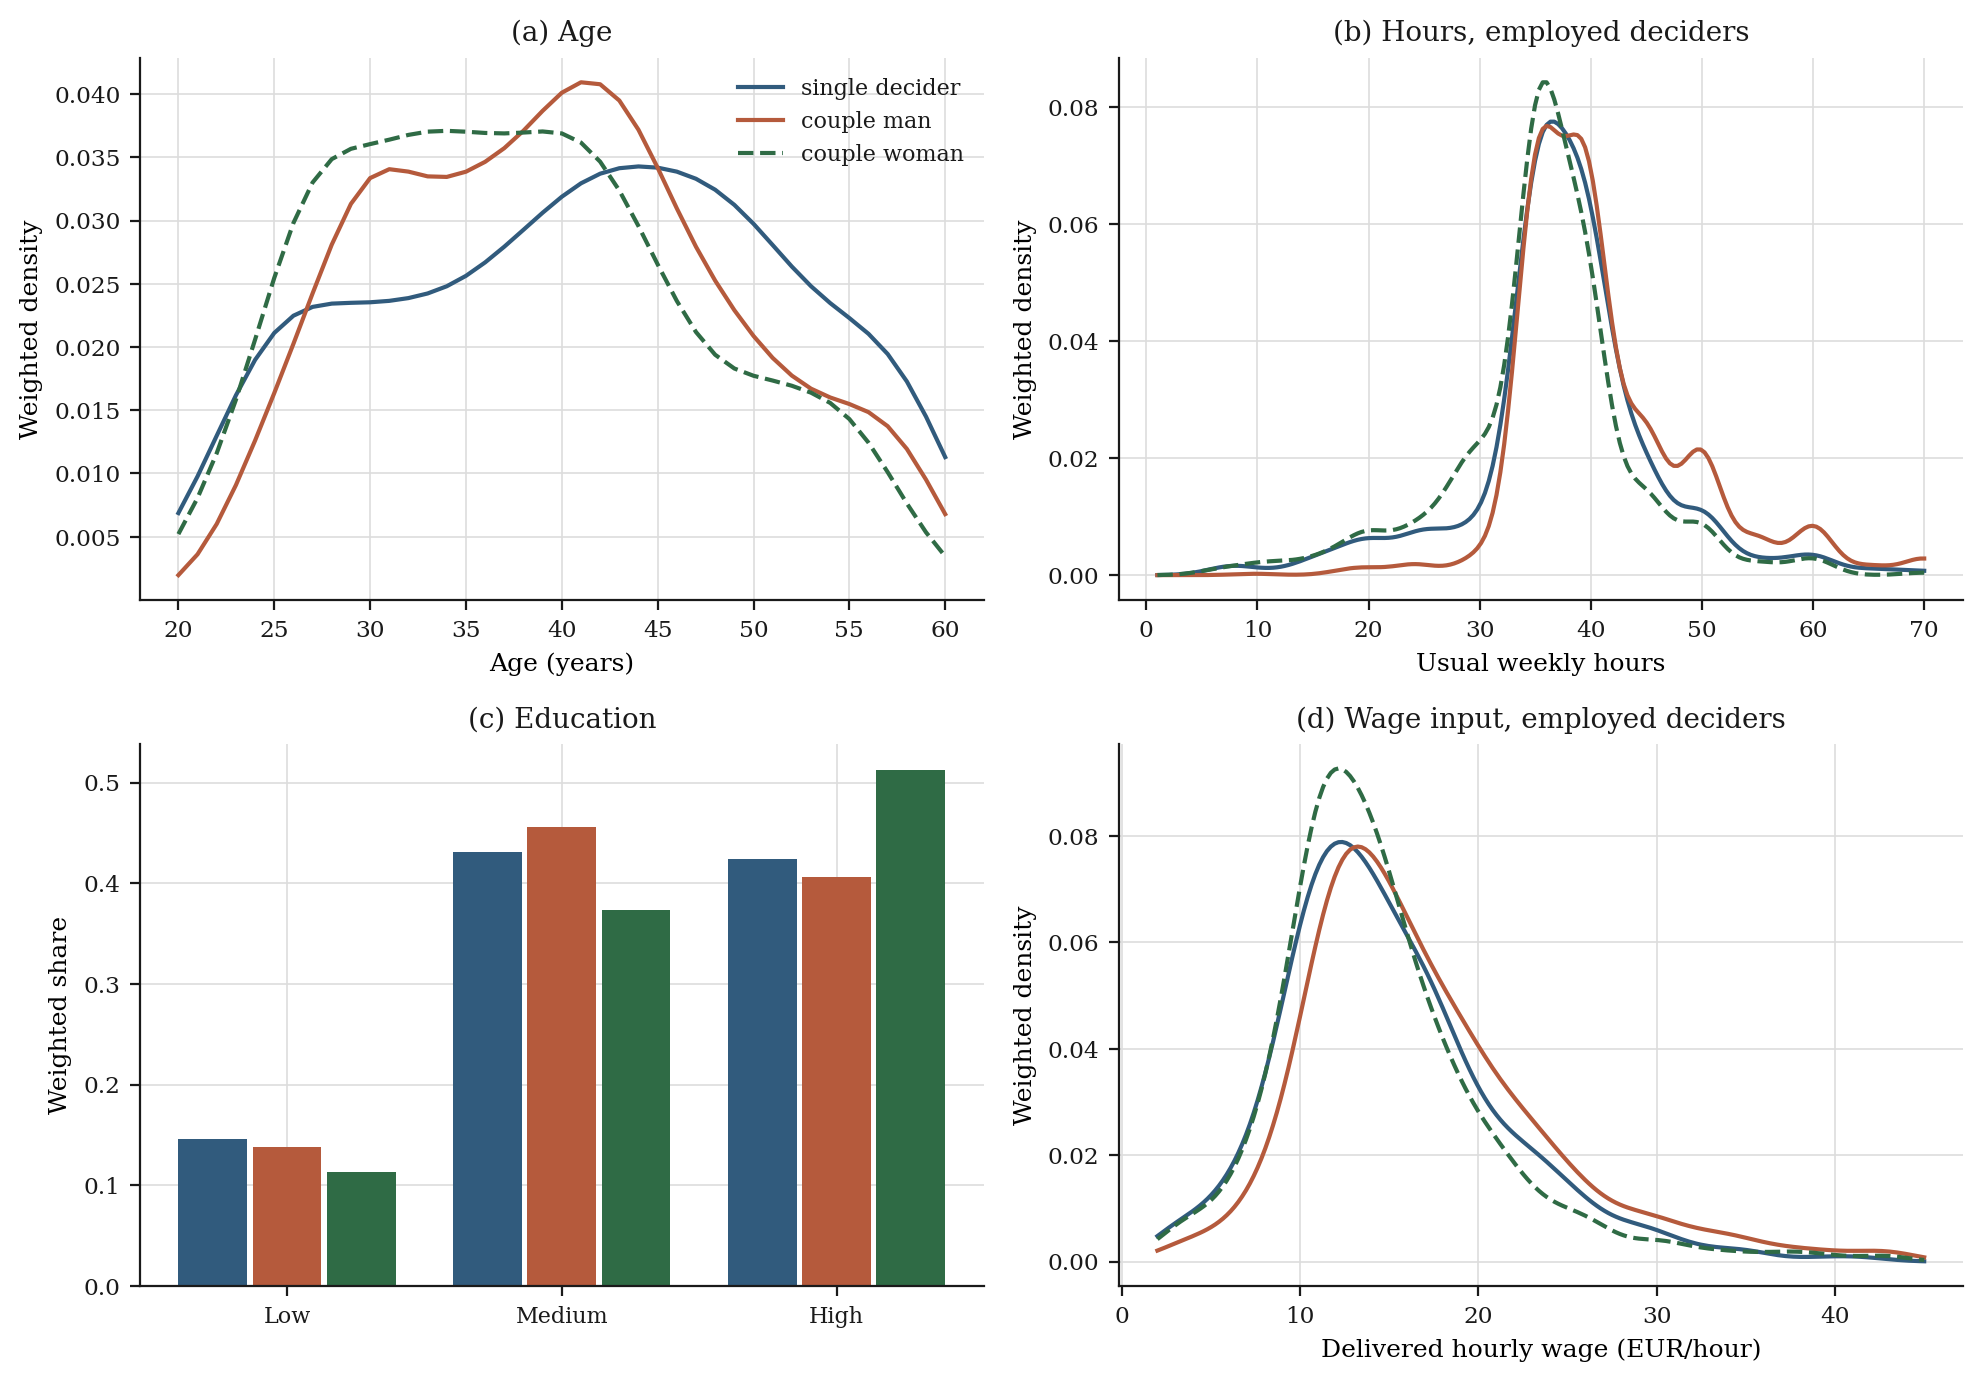
\includegraphics[width=0.95\linewidth,height=\textheight,keepaspectratio,alt={Weighted distributions on the estimation samples: age, usual weekly hours among employed deciders, education, and the delivered hourly wage input. Observed inputs, not model predictions.}]{figures/v5/figV08_data_panel.png}
\caption{Weighted distributions on the estimation samples: age, usual weekly hours among employed deciders, education, and the delivered hourly wage input. Observed inputs, not model predictions.}
\end{figure}

Education is the three-level ISCED grouping, with the medium level as the omitted reference in the wage equation. Potential experience is years since leaving education, entering the wage equation in units of 20 years, with the square recomputed after scaling rather than carried forward. A child is any resident household member under 20, counted without a parent link. Age enters preferences centred on the sample mean decider age and divided by 10 years.

\Needspace*{12\baselineskip}\small\setlength{\tabcolsep}{3pt}\begin{longtable}[]{@{}>{\RaggedRight\arraybackslash}p{0.2500\linewidth}>{\RaggedRight\arraybackslash}p{0.1650\linewidth}>{\RaggedRight\arraybackslash}p{0.1650\linewidth}>{\RaggedRight\arraybackslash}p{0.1650\linewidth}>{\RaggedRight\arraybackslash}p{0.1650\linewidth}@{}}
\caption{Observed joint participation regimes among the 2,223 estimated couple households. These are joint regimes, not two spouse marginals.}\tabularnewline
\toprule\noalign{}
Regime & Meaning & Weighted share & Mean hours, man & Mean hours, woman \\
\midrule\noalign{}
\endfirsthead
\toprule\noalign{}
Regime & Meaning & Weighted share & Mean hours, man & Mean hours, woman \\
\midrule\noalign{}
\endhead
\bottomrule\noalign{}
\endlastfoot
BB & both spouses employed & 0.8435 & 41.0 & 35.9 \\
MO & man employed, woman not employed & 0.0796 & 41.5 & 0.0 \\
WO & woman employed, man not employed & 0.0547 & 0.0 & 35.0 \\
NN & neither spouse employed & 0.0222 & 0.0 & 0.0 \\
\end{longtable}

\subsection{The household budget}\label{the-household-budget}

For a given work arrangement the tax-benefit model is given the implied gross labour inputs, weekly hours, hourly wage, and earnings split at the thirty-five hour threshold, together with the household's non-labour inputs and roster, and returns disposable income. Only deciders receive counterfactual overrides; other members keep their baseline values. The accounting identity linking original income, benefits, taxes and social contributions to disposable income holds to machine precision at both the person and the household-alternative level, before and after the benefit take-up adjustment. Disposable income is summed over all resident members of the household.

\begin{figure}[H]
\centering
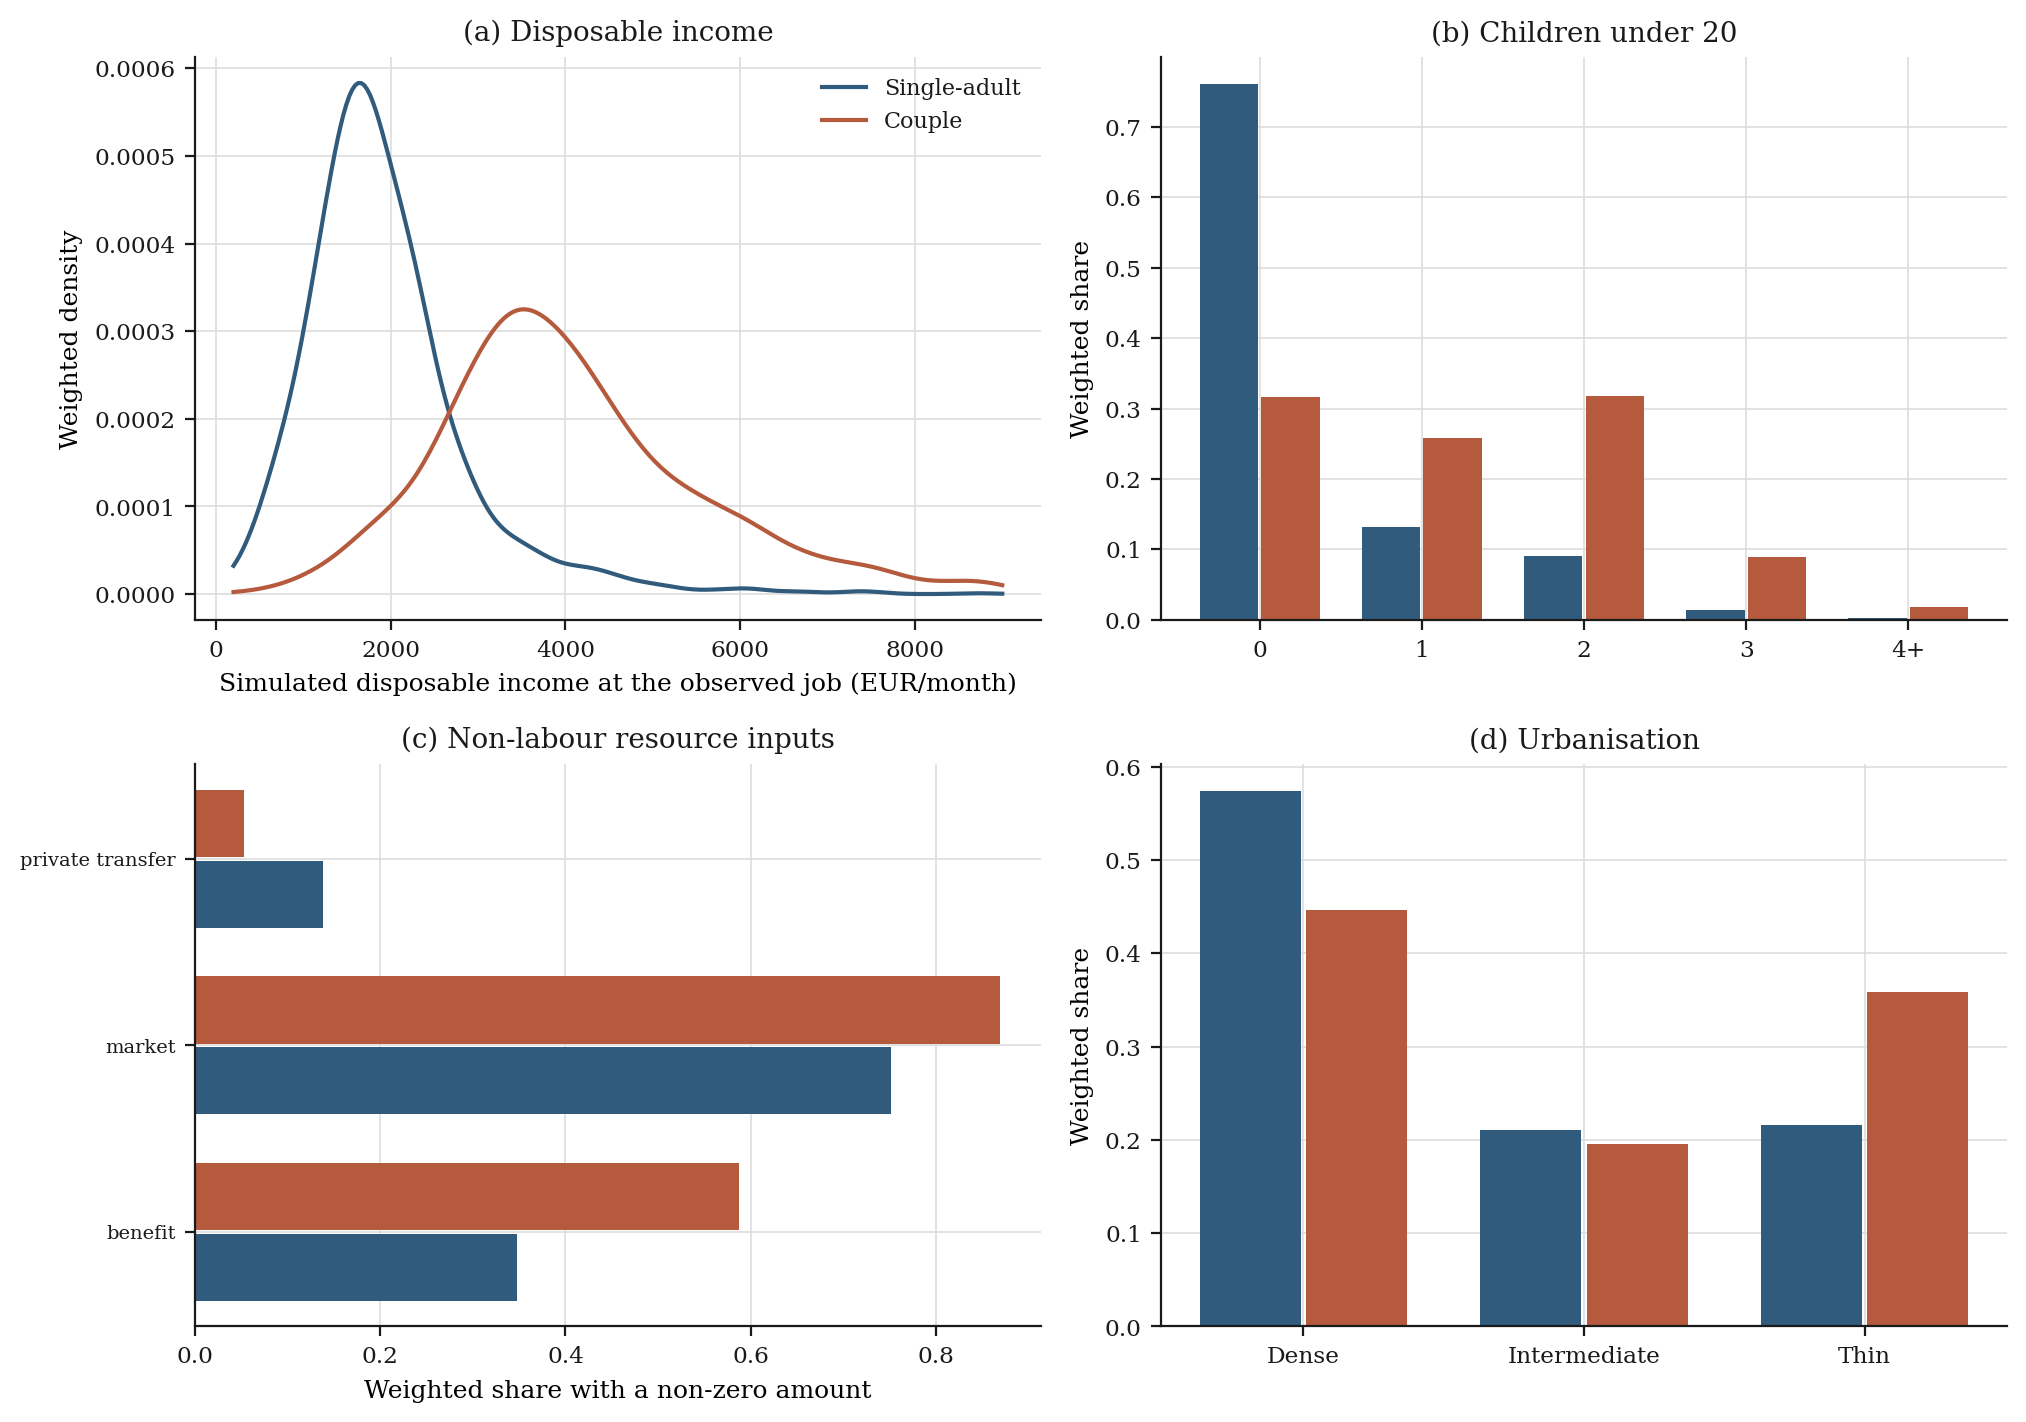
\includegraphics[width=0.95\linewidth,height=\textheight,keepaspectratio,alt={Weighted distributions on the estimation samples: simulated disposable income at the observed job, children under twenty, the incidence of non-labour budget inputs by family, and urbanisation. Panel (a) is a tax-benefit output evaluated at the observed choice; panel (c) reports inputs to that calculation. The two are never added, and stocks are never summed with monthly flows.}]{figures/v5/figV09_resources_panel.png}
\caption{Weighted distributions on the estimation samples: simulated disposable income at the observed job, children under twenty, the incidence of non-labour budget inputs by family, and urbanisation. Panel (a) is a tax-benefit output evaluated at the observed choice; panel (c) reports inputs to that calculation. The two are never added, and stocks are never summed with monthly flows.}
\end{figure}

Panel (c) of the figure reports the \emph{incidence} of non-labour budget inputs by family, not a cash total. Some of these are stocks, some are annual flows and some are monthly; they are inputs to the tax-benefit calculation and are not added together into one income concept. The pension family is empty by construction, because pension receipt is a sample screen. Panel (a) reports the tax-benefit \emph{output} at the observed job, which is an object of a different kind and is never added to panel (c).

Local labour-market conditions enter through a group unemployment measure, a population-weighted exposure index for the decider's region and age-education cell, stored as a fraction and entering the employment index multiplied by 10. Regional and urbanisation variation supports the access specification conditional on the exclusion restriction and the functional form; it does not by itself identify access, and no causal effect of geography is claimed anywhere in this paper.


\section{A latent-jobs model of household labour supply}\label{a-latent-jobs-model-of-household-labour-supply}

A job is a package \(j\): an employment state \(e\in\{0,1\}\) and, when employed, an occupation \(k\in\{1,\dots,4\}\), weekly hours \(h\in[5,70]\) and an hourly wage \(w\in[2,590]\). The base measure \(\nu\) places counting mass on the single non-employment point and, on the employed part, counting measure over occupations with Lebesgue measure over hours and wages. A household chooses one package; a couple chooses one pair of packages under a shared budget.

\subsection{Preferences}\label{preferences}

Let \(C_i(j)\) be priced monthly disposable consumption at \(j\) and \(\ell_i(j)\) normalized leisure, \((80-h)/10\) hours per week, floored at one hour. For a single adult of sex group \(g\), deterministic utility is

\[
u_{ij}=\underbrace{\beta_{\ell}^{g}(\mathbf x_i)\;
\mathcal B\!\left(\tilde\ell_{ij};\theta_{\ell}^{g}\right)}_{L_{ij}}
\;+\;\beta_c\log\tilde c_{ij},
\qquad
\beta_{\ell}^{g}(\mathbf x_i)=\beta_{\ell 0}^{g}+\beta_{\ell a}^{g}a_i
+\beta_{\ell a^{2}}^{g}a_i^{2}
+\mathbb 1\{g=\text{women}\}\,\beta_{\ell k}^{g}k_i,
\]

where \(\mathcal B(z;\theta)=(z^{\theta}-1)/\theta\) with \(\mathcal B(z;0)=\log z\), \(\tilde\ell_{ij}\) is normalized leisure, \(\tilde c_{ij}=C_{ij}/\lambda_c\), \(a_i\) is centred age in decades and \(k_i\) is the child count. For a couple the index is additive across spouses with no direct cross-leisure term,

\[
u_{ij}=\beta_{\ell}^{m}(\mathbf x_i)\,\mathcal B(\tilde\ell^{m}_{ij};\theta_{\ell}^{m})
      +\beta_{\ell}^{f}(\mathbf x_i)\,\mathcal B(\tilde\ell^{f}_{ij};\theta_{\ell}^{f})
      +\beta_c\log\tilde c_{ij},
\]

with consumption the tax-unit sum over all members. We write \(L_i(j)\) throughout for the complete non-consumption part of the index, which for a couple contains both leisure terms.

Three features of this specification are decisions and are worth naming. The consumption curvature is exactly zero, so the consumption term is \(\beta_c\log(C/\lambda_c)\) and the marginal utility of consumption is \(\beta_c/C\), independent of the normalizer. The consumption weight \(\beta_c\) is \textbf{estimated}, not fixed at one. And the random-utility shock is i.i.d. type-I extreme value with scale one, so utility is measured in the natural unit of that scale. Fixing the shock scale is a normalization; additionally fixing \(\beta_c\) would be a substantive restriction relative to that normalization, and estimating \(\beta_c\) removes it. Neither step identifies an absolute cardinal utility scale, and fixing the consumption functional form is not by itself what identifies the shock scale.

The normalizer \(\lambda_c\) is a units convention. Under exact log consumption it enters the index as the alternative-invariant constant \(-\beta_c\log\lambda_c\), so it cancels from every choice probability and, as shown below, exactly from the welfare measure.

\subsection{Opportunities}\label{opportunities}

The opportunity density gives the relative intensity with which packages are available to household \(i\), before any choice is made. It is a product of \textbf{four} factors, switched off on non-employment by the employment indicator \(E_{ij}=\mathbb 1\{h_{ij}>0\}\):

\[
g_{ij}=g^{E}_{ij}\cdot\left(g^{H}_{ij}\cdot g^{\mathrm{Occ}}_{ij}\cdot g^{W}_{ij}\right)^{E_{ij}} .
\]

\textbf{Access}, \(g^{E}_{ij}=\exp\{\beta_E+\beta_s s_i+\sum_{r=2}^{8}\beta_r\,\mathrm{reg}_{ir}+\beta_u u_i+\beta_m m_i\}\), carries the local group unemployment measure \(s_i\), the region indicators and urbanisation, and is the factor inside which local-market access lives. \textbf{Hours}, \(g^{H}_{ij}=\exp\{\sum_b \beta_b\mathbb 1\{h_{ij}\in b\}\}\), elevates five bands over a residual reference set of total width 26.5 hours per week, so every band coefficient is read against that residual and none of the five is normalized to zero; the narrow full-time band \([33.5,36.5)\) is a density elevation over an interval, not an atom at thirty-five hours. \textbf{Occupation}, \(g^{\mathrm{Occ}}_{ij}=\exp\{\beta^{\mathrm{occ}}_{k,g}\}\) with \(\beta^{\mathrm{occ}}_{1,g}\equiv 0\). \textbf{Wage offer}, \(g^{W}_{ij}\), is log-normal with location \(\mu_i=\beta_{w0}+\beta_{wL}L_i+\beta_{wH}H_i+\beta_{wx}x_i+\beta_{wx^{2}}x_i^{2}+\delta_{\mathrm{occ}}\) and dispersion \(\sigma\), truncated to \([2,590]\) euros per hour and renormalized on that support.

Two properties of the normalization matter later. Write \(\widehat g_{ij}=g_{ij}/Z_i\) for the density normalized to unit mass on the whole package space. The wage factor integrates to one \emph{conditional on employment and occupation}, because the truncated density is renormalized on its own support; and the non-consumption index \(L_{ij}\) has no wage argument. Together these give the reference the pay-neutrality property established in Section 4.

The four blocks are what the decomposition later separates. Employment and occupation access are one mechanism; the distribution of wages conditional on an occupation is another; neither is the same as non-labour resources or household needs.

\subsection{Identification, in words}\label{identification-in-words}

Choices alone do not separate a taste for leisure from a scarcity of jobs at that number of hours. Three kinds of restriction do the work. Preferences are smooth in hours through the leisure index, while the opportunity density is a step function over bands, so a spike in observed hours at a band is read as availability rather than as a kink in tastes. Excluded shifters enter availability and not preferences: the local group unemployment measure and the regional and urbanisation indicators shift the employment index and appear nowhere in utility. And the wage-offer distribution is specified as independent of offered hours conditional on occupation, which separates the wage location from the hours density. These are the restrictions of \citet{capeau2016} and \citet{dagsvikjia2016}, maintained here rather than tested. The regional variation supports the access block conditional on those restrictions; it does not establish separate identification on its own, and it is not a causal design.

\subsection{Estimation}\label{estimation}

The choice set is a continuum, so the likelihood is evaluated over sampled alternatives. For each household we draw \(R=100\) alternatives from a proposal density \(q_{ij}\) and place the observed package in the set as well, giving a set \(\mathcal C_i\) with \(|\mathcal C_i|=101\) rows. Write the sampled-set index

\[
V_{ij}=u_{ij}+\log g_{ij}-\log q_{ij},
\qquad
q_{ij}=q^{E}_{ij}\left(q^{H}_{ij}q^{W}_{ij}q^{\mathrm{Occ}}_{ij}\right)^{E_{ij}} .
\]

The contribution of household \(i\) is then the conditional probability of its observed package \(y\) within that set,

\[
\Pr\!\left(y\mid\mathcal C_i\right)=
\frac{n_{y}\exp V_{iy}}{\sum_{s\in\mathcal C_i}\exp V_{is}} .
\]

The denominator runs over slots rather than distinct packages, and a package drawn more than once keeps its multiplicity, \(n_y\); the observed package carries the same proposal correction as any other row. The proposal density is a computational device and never an economic object: it is not an offer, an availability or an opportunity. The proposal is fitted out of fold, so a household's own outcome never enters the proposal used to score it. For couples the proposal draws the joint participation regime first and then the two spouse packages conditional on it.

Standard errors are cluster-robust on the household. Optimization uses five starts under two polishing contracts, ten terminal paths in all; we report the spread of the criterion across those paths and the eigenvalues of the exact Hessian at the selected optimum. Those diagnostics support a stable local solution found from the starts tested. They are not a proof of global uniqueness, and we do not claim one.

Two features of the observation rule remain genuinely open and are stated here rather than in a footnote. The sample screens on the observed hours and wage of employed deciders, so the estimation sample is selected on an outcome of the process being modelled. The conditional likelihood above is the correct object for a sampled choice set; it is not automatically the correct object for an outcome-selected sample, and we have not established which correction, if any, the screen requires. Separately, the derivation of the sampled-set probability conditions on a labelled collection of slots; small observed cross-coordinate correlations and a binomial-looking multiplicity distribution are consistent with independent draws but do not by themselves establish the sampling law. Both are recorded as unresolved in Section 6.


\section{Money-metric well-being and structural inequality decomposition}\label{money-metric-well-being-and-structural-inequality-decomposition}

\subsection{The measure}\label{the-measure}

Fix a household \(i\) and a coalition state \(S\), which determines the utility index \(L_{i,S}\), the normalized opportunity density \(\widehat g_{i,S}\) and the priced consumption \(C_{i,S}\) at every package. Define the attained ex-ante value and the reference mass

\[
J_{i,S}=\int e^{L_{i,S}(j)}\left(\frac{C_{i,S}(j)}{\lambda_c}\right)^{\beta_c}\widehat g_{i,S}(j)\,d\nu(j),
\qquad
H_{i,S}=\int e^{L_{i,S}(j)}\,\widehat g_{i,S}(j)\,d\nu(j).
\]

The reference offers the same flat monthly amount \(m\) at every package while retaining that state's \(L\) and \(\widehat g\), so the value of the reference is

\[
\Phi_{i,S}(m)=\beta_c\log(m/\lambda_c)+\log H_{i,S},
\qquad \Phi_{i,S}'(m)=\beta_c/m>0 .
\]

The money metric is the amount at which the reference reaches the attained value, \(\Phi_{i,S}(W_{i,S})=\log J_{i,S}\), which inverts in closed form:

\[
\boxed{\;W_{i,S}=\lambda_c\exp\!\left[\frac{\log J_{i,S}-\log H_{i,S}}{\beta_c}\right].\;}
\]

Writing \(r_{i,S}(dj)=e^{L_{i,S}(j)}\widehat g_{i,S}(j)\,d\nu(j)/H_{i,S}\) for the reference probability measure, the same object is

\[
\boxed{\;W_{i,S}=\left[\int C_{i,S}(j)^{\beta_c}\,r_{i,S}(dj)\right]^{1/\beta_c}.\;}
\]

The measure is therefore a \textbf{weighted power mean of consumption of order \(\beta_c\)}, taken under a reference measure that weights packages by their non-consumption value and their availability. It is an arithmetic mean only at \(\beta_c=1\). The normalizer \(\lambda_c\) cancels between the two forms, which is why the constant is a units convention and not a modelling choice; we verify this numerically to a maximum relative deviation of 2.7e-15 across four widely separated values.

\begin{figure}[H]
\centering
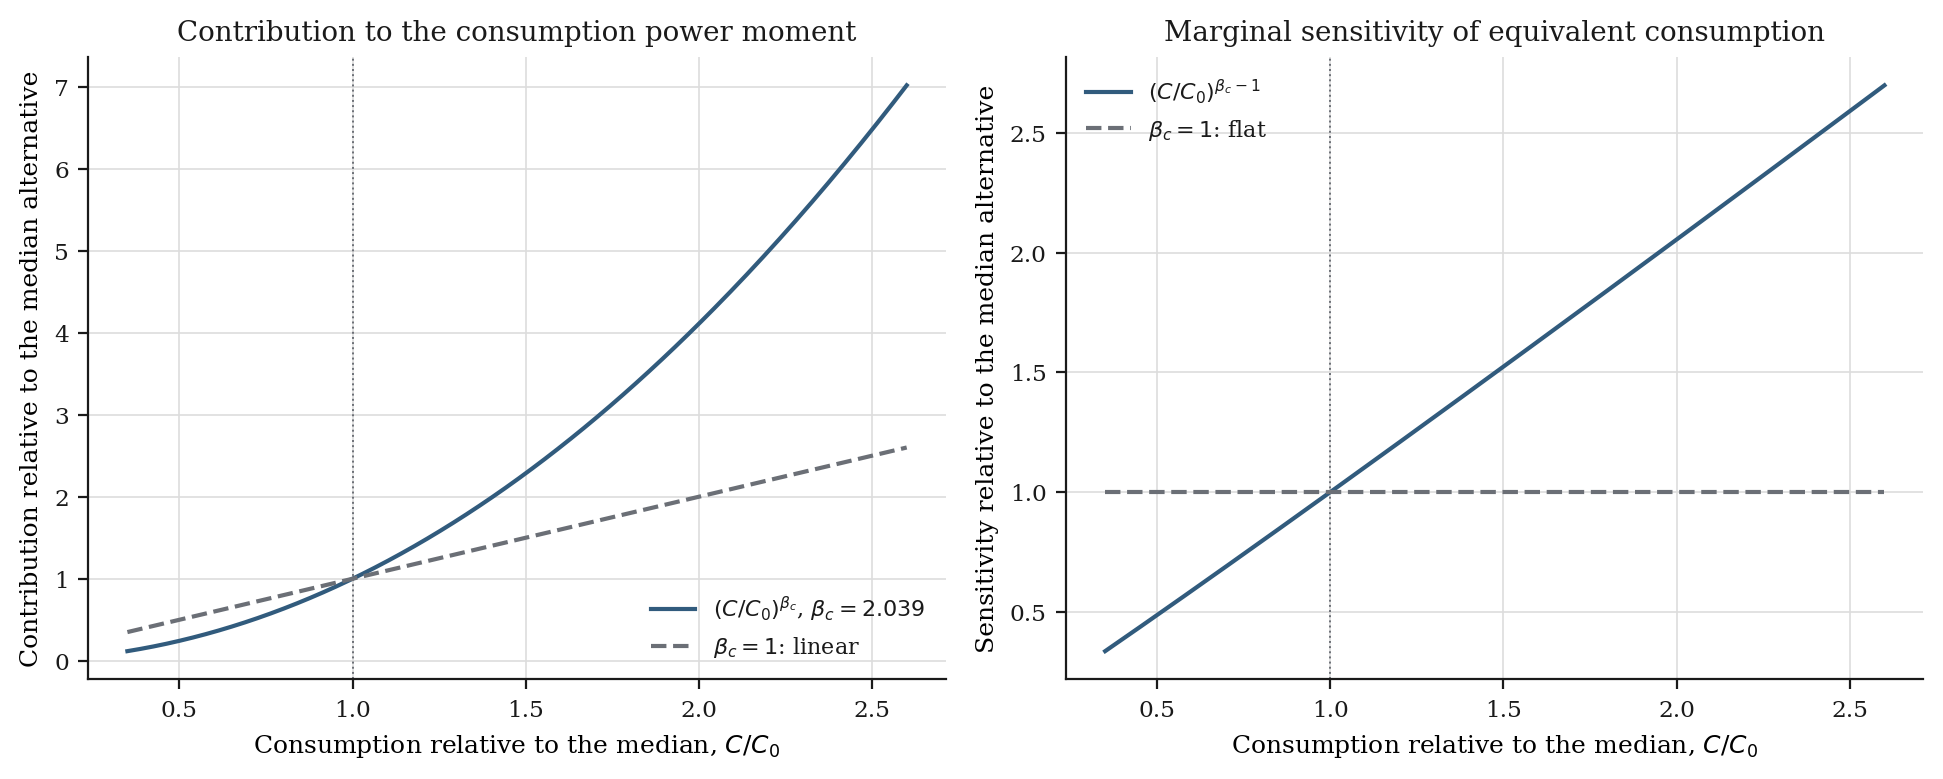
\includegraphics[width=0.95\linewidth,height=\textheight,keepaspectratio,alt={The consumption coefficient as the order of a power mean. Left: the contribution an alternative makes to the consumption power moment, relative to the median alternative, against the linear comparison at \textbackslash beta\_c=1. Right: the marginal effect of that alternative's consumption on the resulting equivalent amount, which carries exponent \textbackslash beta\_c-1, against the flat comparison at \textbackslash beta\_c=1. Neither curve is a reference probability weight: holding the reference measure fixed, those weights do not vary with consumption at all.}]{figures/v5/figV07_power_mean.png}
\caption{The consumption coefficient as the order of a power mean. Left: the contribution an alternative makes to the consumption power moment, relative to the median alternative, against the linear comparison at \(\beta_c=1\). Right: the marginal effect of that alternative's consumption on the resulting equivalent amount, which carries exponent \(\beta_c-1\), against the flat comparison at \(\beta_c=1\). Neither curve is a reference probability weight: holding the reference measure fixed, those weights do not vary with consumption at all.}
\end{figure}

Three quantities are easy to conflate and are distinct. The reference probability weight \(r_j\) does not vary with consumption at all when the reference measure is held fixed. The \emph{contribution} an alternative makes to the power moment is proportional to \(C_j^{\beta_c}\), so an alternative paying twice the median contributes 4.11 times as much at the estimated single-adult coefficient. The \emph{marginal effect} of that alternative's consumption on the resulting amount is \(\partial W/\partial C_j=r_jC_j^{\beta_c-1}W^{1-\beta_c}\), with exponent \(\beta_c-1\). The figure plots the second and the third and labels each; neither is a statement that the alternative is more available.

\(\beta_c\) is the order of this power mean and the coefficient on log consumption. It is not the consumption curvature, which is exactly zero here, and it is not an inequality-aversion parameter across households, which belongs to the index applied in Section 5 and not to the household's own aggregator.

\subsection{What the reference does and does not do to pay}\label{what-the-reference-does-and-does-not-do-to-pay}

Under the stated factorization the reference is invariant to the conditional wage density: that density integrates to one on its support and the non-consumption index has no wage argument, so replacing it leaves \(H_{i}\) unchanged. Numerically, the largest household change in \(\log H\) is 1.8e-15 for single adults and 7.1e-15 for couples, and the median change in the money metric through the direct reference channel is exactly 0 euros.

Changes in earning opportunities nevertheless change the measure, because they change what the household attains: the median total change is -17.43 euros per month for single adults and 110.53 for couples. The correct statement is therefore narrow and we make only it: \emph{the reference is directly pay-neutral, and earning opportunities reach the measure through the attained evaluation.} A total change that travels through attainment does not establish that the deterministic independence-of-pay axiom fails for this stochastic functional. That would require fixing the primitives the axiom holds fixed and proving the property, which we have not done and do not claim.

\subsection{Interpersonal comparison and the unit}\label{interpersonal-comparison-and-the-unit}

The measure is defined at the household. Comparing households of different size requires an equivalence scale, which is a normative choice and not an estimate. We report every result on two bases: a raw household basis, and an equivalized basis using the modified OECD scale. We never pool the two household types into one distribution, because the two applications carry different reference constructions and the levels are not comparable; every share below is a share of the baseline inequality of its own population.

\subsection{The structural decomposition}\label{the-structural-decomposition}

Let \(X_i=(P_i,A_i,B_i,D_i)\) collect the four structural inputs for household \(i\):

\begin{itemize}
\tightlist
\item
  \(P_i\) the arguments of the preference index: the leisure-weight covariates and the sex- or spouse-specific preference block;
\item
  \(A_i\) the arguments of job access: the employment index covariates and the occupation access table;
\item
  \(B_i\) the arguments of earning opportunities: the covariates entering the offered-wage location;
\item
  \(D_i\) the household budget inputs: non-labour resources, the roster and needs.
\end{itemize}

Let \(\mathcal I\) be an inequality index and \(W_i(\cdot)\) the money metric of the previous subsection, so that the baseline is \(I_\varnothing=\mathcal I\{W_i(X_i)\}_{i=1}^N\). For each factor define a \textbf{structural equalization operator} \(T_P,T_A,T_B,T_D\), which replaces that factor's arguments across all households by a common reference profile and leaves the estimated coefficients in place. For a coalition \(S\subseteq\{P,A,B,D\}\) let \(X^S=T_S(X)\) be the state in which exactly the factors in \(S\) are equalized, and set

\[
I_S=\mathcal I\{W_i(T_S X)\}_{i=1}^{N},
\qquad
v(S)=I_\varnothing-I_S .
\]

\(v\) is a cooperative game on four players: the worth of a coalition is the inequality it removes when its factors are equalized together. Two points about \(T_S\) are part of the economics and not of the notation. First, \(T_S\) is a single simultaneous substitution map, not an ordered product \(\prod_{k\in S}T_k\): a product is not well defined unless the operators commute on the permitted objects, and the budget operator does not commute with the others, since it reprices. Second, an operator changes a \emph{pathway}, not every occurrence of a raw characteristic. Education enters both the offered-wage location and the local-market lookup; \(T_B\) substitutes the first and leaves the second in place.

\Needspace*{12\baselineskip}\small\setlength{\tabcolsep}{3pt}\begin{longtable}[]{@{}
  >{\raggedright\arraybackslash}p{(\linewidth - 6\tabcolsep) * \real{0.2500}}
  >{\raggedright\arraybackslash}p{(\linewidth - 6\tabcolsep) * \real{0.2500}}
  >{\raggedright\arraybackslash}p{(\linewidth - 6\tabcolsep) * \real{0.2500}}
  >{\raggedright\arraybackslash}p{(\linewidth - 6\tabcolsep) * \real{0.2500}}@{}}
\caption{The four structural equalization operators. Each operator replaces the arguments of one structural pathway with a common reference profile and leaves the estimated coefficients in place; it does not equalize every occurrence of a raw characteristic. Education, for example, enters both the wage location and the local-market lookup, and only the named pathway is substituted. Operators are applied as one simultaneous substitution map, not as an ordered product.}\tabularnewline
\toprule\noalign{}
\begin{minipage}[b]{\linewidth}\raggedright
Operator
\end{minipage} & \begin{minipage}[b]{\linewidth}\raggedright
What is replaced
\end{minipage} & \begin{minipage}[b]{\linewidth}\raggedright
What is retained
\end{minipage} & \begin{minipage}[b]{\linewidth}\raggedright
Repricing
\end{minipage} \\
\midrule\noalign{}
\endfirsthead
\toprule\noalign{}
\begin{minipage}[b]{\linewidth}\raggedright
Operator
\end{minipage} & \begin{minipage}[b]{\linewidth}\raggedright
What is replaced
\end{minipage} & \begin{minipage}[b]{\linewidth}\raggedright
What is retained
\end{minipage} & \begin{minipage}[b]{\linewidth}\raggedright
Repricing
\end{minipage} \\
\midrule\noalign{}
\endhead
\bottomrule\noalign{}
\endlastfoot
\(T_P\) preferences & Singles: the arguments of the leisure weight and the complete reference-sex leisure block. Couples: the medoid spouse arguments, with own spouse coefficients retained & Budget roster, resources, access and wage pathways of the same characteristics & No: pure utility shifters do not change the budget \\
\(T_A\) job access & The arguments of the employment index and the occupation access table & Preferences, wage location, budget inputs; sex-specific occupation coefficients & No: the priced jobs are unchanged \\
\(T_B\) earning opportunities & The arguments of the offered-wage location: education shares and experience moments, with squares recomputed rather than averaged & The estimated wage coefficients and dispersion; the preference and access pathways of the same characteristics & No on a common priced node set: the change is in the density over nodes \\
\(T_D\) resources and needs & The non-labour budget inputs, the household roster and the needs profile & Every non-budget structural pathway & Yes: the household budget is recomputed through the tax-benefit system \\
\end{longtable}

Welfare and inequality are then recomputed from the model for all sixteen coalitions. There is no linearisation and no re-estimation: coefficients are held at their estimates throughout, and only the arguments move. The budget operator additionally reruns the household through the tax-benefit system, so its counterfactual consumption is priced rather than scaled.

The interactions are allocated with the \textbf{grouped Shapley--Owen--Shorrocks} rule for the partition \(\{\{P\},\{A,B,D\}\}\): the Owen value \citep{owen1977} for a game with a priori unions, applied to \(v\) in the form \citet{shorrocks2013} sets out for distributional analysis and \citet{audoly2025} document for grouped nonlinear decompositions. The grouping is chosen because the paper's question is first about preferences against circumstances and only then about which circumstance; the lower-level subdivision of \(\{A,B,D\}\) is allocated within the union. The allocation is exhaustive: the contributions sum to \(I_\varnothing-I_{\{P,A,B,D\}}\), and \(I_{\{P,A,B,D\}}\) is zero to numerical precision. We verify that closure rather than imposing it; residuals are reported in Section 5.


\section{Empirical results}\label{empirical-results}

\subsection{Behavioural estimates}\label{behavioural-estimates}

The estimated model has 41 free coordinates for single adults, of which 40 are interior, and 47 for couples, all interior. The criterion is 6253.463 and 10283.034 respectively. Across ten terminal paths from five starts under two polishing contracts, the criterion varies by 1.1e-10 for single adults and 1.3e-09 for couples, and the smallest eigenvalue of the exact Hessian on the interior block is 0.1669 and 0.0771. One single-adult coordinate, the female age-square term in the leisure weight, sits at a box endpoint; its interval is reported under the active-set convention in the appendix and it is excluded from the interior curvature.

\Needspace*{12\baselineskip}\small\setlength{\tabcolsep}{3pt}\begin{longtable}[]{@{}
  >{\raggedright\arraybackslash}p{(\linewidth - 8\tabcolsep) * \real{0.2000}}
  >{\raggedright\arraybackslash}p{(\linewidth - 8\tabcolsep) * \real{0.2000}}
  >{\raggedright\arraybackslash}p{(\linewidth - 8\tabcolsep) * \real{0.2000}}
  >{\raggedright\arraybackslash}p{(\linewidth - 8\tabcolsep) * \real{0.2000}}
  >{\raggedright\arraybackslash}p{(\linewidth - 8\tabcolsep) * \real{0.2000}}@{}}
\caption{The preference block. Cluster-robust standard errors in parentheses, clustered on the household. ``At bound'' marks an estimate at a box endpoint, whose interval is reported under the active-set convention in the appendix. The consumption weight is common within a population and enters as \(\beta_c\log(C/\lambda_c)\).}\tabularnewline
\toprule\noalign{}
\begin{minipage}[b]{\linewidth}\raggedright
Coefficient
\end{minipage} & \begin{minipage}[b]{\linewidth}\raggedright
Single men
\end{minipage} & \begin{minipage}[b]{\linewidth}\raggedright
Single women
\end{minipage} & \begin{minipage}[b]{\linewidth}\raggedright
Couple men
\end{minipage} & \begin{minipage}[b]{\linewidth}\raggedright
Couple women
\end{minipage} \\
\midrule\noalign{}
\endfirsthead
\toprule\noalign{}
\begin{minipage}[b]{\linewidth}\raggedright
Coefficient
\end{minipage} & \begin{minipage}[b]{\linewidth}\raggedright
Single men
\end{minipage} & \begin{minipage}[b]{\linewidth}\raggedright
Single women
\end{minipage} & \begin{minipage}[b]{\linewidth}\raggedright
Couple men
\end{minipage} & \begin{minipage}[b]{\linewidth}\raggedright
Couple women
\end{minipage} \\
\midrule\noalign{}
\endhead
\bottomrule\noalign{}
\endlastfoot
Leisure weight, intercept \(\beta_{\ell 0}\) & 8.5199 (3.5480) & 5.8683 (2.1346) & 3.9814 (0.7466) & 13.1029 (4.7760) \\
Leisure weight, age \(\beta_{\ell a}\) & 1.4820 (1.0236) & 0.0678 (0.4792) & -0.0080 (0.0287) & -0.1228 (0.1260) \\
Leisure weight, age squared \(\beta_{\ell a^2}\) & 0.7783 (0.7732) & 1.0000 (at bound) & 0.0065 (0.0030) & 0.0073 (0.0103) \\
Leisure weight, children \(\beta_{\ell n}\) & --- & 0.1666 (0.4422) & --- & -0.3055 (1.1472) \\
Leisure curvature \(\theta_\ell\) & -1.6263 (0.3301) & -0.9274 (0.2161) & -0.9761 (0.1357) & -1.6863 (0.2458) \\
Consumption weight \(\beta_c\) & 2.0387 (0.2917) & 2.0387 (0.2917) & 2.1017 (0.2939) & 2.1017 (0.2939) \\
\end{longtable}

The consumption weight is 2.0387 with a cluster-robust standard error of 0.2917 for single adults and 2.1017 with 0.2939 for couples. Two things follow. Because the estimate exceeds one, the money metric of Section 4 is a power mean of order above one rather than an arithmetic mean. And because utility is on the unit-scale shock, one natural unit of the index corresponds to multiplying consumption by \(\exp(1/\beta_c)\), a factor of 1.633 for single adults and 1.609 for couples. That is a proportional statement: there is no single euro value of a unit of utility independent of the consumption at which it is evaluated.

\Needspace*{12\baselineskip}\small\setlength{\tabcolsep}{3pt}\begin{longtable}[]{@{}
  >{\raggedright\arraybackslash}p{(\linewidth - 6\tabcolsep) * \real{0.2500}}
  >{\raggedright\arraybackslash}p{(\linewidth - 6\tabcolsep) * \real{0.2500}}
  >{\raggedright\arraybackslash}p{(\linewidth - 6\tabcolsep) * \real{0.2500}}
  >{\raggedright\arraybackslash}p{(\linewidth - 6\tabcolsep) * \real{0.2500}}@{}}
\caption{The opportunity block: employment access, the hours density and occupation access. Cluster-robust standard errors in parentheses. The employment index multiplies the working indicator; the omitted references are region 1, thinly populated areas, the residual hours set of total width 26.5 hours per week, and occupation group 1. The singles occupation column reports the female coordinates; the male coordinates are in the appendix table. Hours coefficients are common across the two singles sex groups and spouse-specific for couples.}\tabularnewline
\toprule\noalign{}
\begin{minipage}[b]{\linewidth}\raggedright
Coefficient
\end{minipage} & \begin{minipage}[b]{\linewidth}\raggedright
Singles
\end{minipage} & \begin{minipage}[b]{\linewidth}\raggedright
Couple men
\end{minipage} & \begin{minipage}[b]{\linewidth}\raggedright
Couple women
\end{minipage} \\
\midrule\noalign{}
\endfirsthead
\toprule\noalign{}
\begin{minipage}[b]{\linewidth}\raggedright
Coefficient
\end{minipage} & \begin{minipage}[b]{\linewidth}\raggedright
Singles
\end{minipage} & \begin{minipage}[b]{\linewidth}\raggedright
Couple men
\end{minipage} & \begin{minipage}[b]{\linewidth}\raggedright
Couple women
\end{minipage} \\
\midrule\noalign{}
\endhead
\bottomrule\noalign{}
\endlastfoot
Employment constant \(\beta_E\) & -3.1735 (0.4053) & -2.1233 (0.3195) & -2.8148 (0.3021) \\
Group unemployment rate \(\beta_{E,gsur}\) & -1.4422 (0.2356) & -1.1924 (0.1557) & shared with the man \\
Densely populated \(\beta_{E,u}\) & -0.0288 (0.2209) & -0.1823 (0.1657) & shared with the man \\
Intermediate density \(\beta_{E,m}\) & 0.0641 (0.2614) & -0.4174 (0.1861) & shared with the man \\
Region 2 \(\beta_{E,2}\) & -0.3780 (0.3292) & -0.1546 (0.2442) & shared with the man \\
Region 3 \(\beta_{E,3}\) & -0.1117 (0.3891) & 0.0873 (0.2808) & shared with the man \\
Region 4 \(\beta_{E,4}\) & -0.8218 (0.3810) & 0.0150 (0.3068) & shared with the man \\
Region 5 \(\beta_{E,5}\) & -0.5162 (0.3274) & -0.1455 (0.2555) & shared with the man \\
Region 6 \(\beta_{E,6}\) & -0.7222 (0.3528) & -0.2844 (0.2748) & shared with the man \\
Region 7 \(\beta_{E,7}\) & -0.5374 (0.3503) & -0.1396 (0.2651) & shared with the man \\
Region 8 \(\beta_{E,8}\) & -0.4512 (0.3401) & -0.1659 (0.2660) & shared with the man \\
Hours band: Part-time lower, {[}17.5, 21.5) & 0.0298 (0.1972) & -1.1094 (0.3791) & -0.5173 (0.1629) \\
Hours band: Part-time upper, {[}28.5, 30.5) & 0.7080 (0.1928) & 0.0835 (0.2378) & 1.1586 (0.1214) \\
Hours band: Narrow full-time, {[}33.5, 36.5) & 2.0656 (0.0894) & 2.2888 (0.0821) & 2.0284 (0.0682) \\
Hours band: Full-time upper, {[}36.5, 40.5{]} & 1.9387 (0.0997) & 2.3801 (0.0866) & 1.6825 (0.0798) \\
Hours band: Long hours, {[}44.5, 70{]} & -0.0834 (0.1772) & 0.6977 (0.1335) & -0.3109 (0.1615) \\
Occupation 2 \(\xi_2\) & 0.1135 (0.1374) & -1.5097 (0.0967) & 0.2074 (0.0891) \\
Occupation 3 \(\xi_3\) & -0.4060 (0.1440) & -2.2532 (0.1244) & -0.1804 (0.0923) \\
Occupation 4 \(\xi_4\) & 0.5632 (0.1225) & 0.1594 (0.0618) & 0.8159 (0.0799) \\
\end{longtable}

\Needspace*{12\baselineskip}\small\setlength{\tabcolsep}{3pt}\begin{longtable}[]{@{}>{\RaggedRight\arraybackslash}p{0.4200\linewidth}>{\RaggedRight\arraybackslash}p{0.2590\linewidth}>{\RaggedRight\arraybackslash}p{0.2590\linewidth}@{}}
\caption{The wage block and the consumption weight. The offered log wage is normal with mean \(\mu_i(k)\) and dispersion \(\sigma\), truncated to {[}2, 590{]} EUR/hour and renormalized on that support. Experience enters in units of twenty years. Slopes and \(\sigma\) are common across the two singles sex groups and across spouses within couples; the singles and couples models are estimated separately, so the two columns are not restricted to agree.}\tabularnewline
\toprule\noalign{}
Coefficient & Singles & Couples \\
\midrule\noalign{}
\endfirsthead
\toprule\noalign{}
Coefficient & Singles & Couples \\
\midrule\noalign{}
\endhead
\bottomrule\noalign{}
\endlastfoot
Intercept \(\beta_{w0}\) & 2.0138 (0.0561) & 2.0480 (0.0335) \\
Low education \(\beta_{wL}\) & 0.0566 (0.0372) & -0.0433 (0.0217) \\
High education \(\beta_{wH}\) & 0.1491 (0.0308) & 0.1817 (0.0197) \\
Potential experience \(\beta_{wx}\) & 0.2408 (0.0862) & 0.5643 (0.0546) \\
Experience squared \(\beta_{wx^2}\) & -0.0282 (0.0390) & -0.1598 (0.0243) \\
Occupation 2 \(\delta_2\) & -0.0347 (0.0399) & -0.0740 (0.0231) \\
Occupation 3 \(\delta_3\) & 0.0622 (0.0383) & 0.0394 (0.0228) \\
Occupation 4 \(\delta_4\) & 0.2785 (0.0368) & 0.2146 (0.0223) \\
Log-wage dispersion \(\sigma\) & 0.3815 (0.0133) & 0.3631 (0.0072) \\
Consumption weight \(\beta_c\) & 2.0387 (0.2917) & 2.1017 (0.2939) \\
\end{longtable}

\textbf{Maintained restrictions.} Singles: \texttt{theta\_c\_singles\ =\ 0}; the couples preference block (\texttt{beta\_l0\_m}, \texttt{beta\_l\_age\_m}, \texttt{beta\_l\_age2\_m}, \texttt{beta\_l0\_f}, \texttt{beta\_l\_age\_f}, \texttt{beta\_l\_age2\_f}, \texttt{beta\_l\_nkids\_f}, \texttt{theta\_l\_f}) does not enter the singles likelihood; and \texttt{beta\_E\_y2015} and \texttt{beta\_E\_y2017} are absent because the 2015 and 2017 data are not used. Couples: \texttt{theta\_c\ =\ 0}, the male children leisure effect is structurally zero, and the direct cross-leisure term is fixed at zero. These are restrictions, not estimates. The singles and couples models are estimated separately, so their wage blocks are not restricted to agree, and the difference between the two experience profiles should not be read as a test.

\begin{figure}[H]
\centering
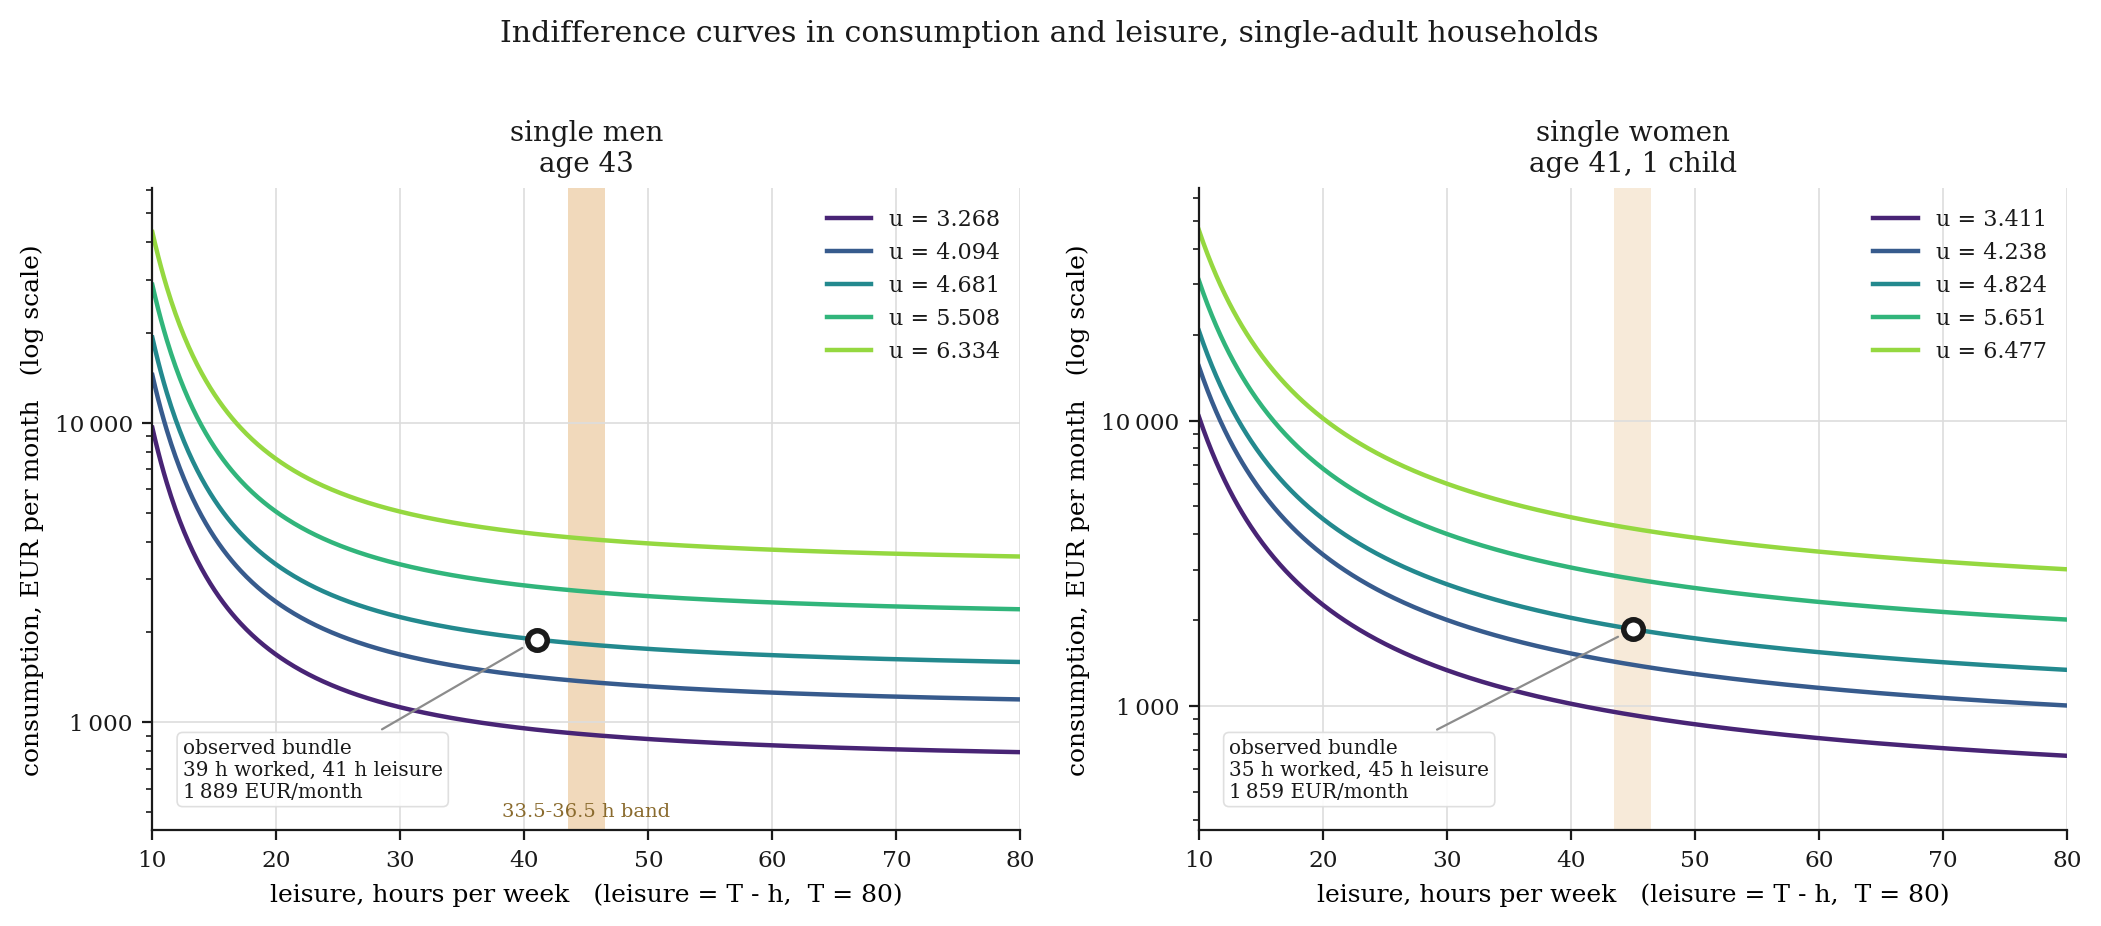
\includegraphics[width=0.95\linewidth,height=\textheight,keepaspectratio,alt={Indifference curves in consumption and leisure, single-adult households, at one representative household of each sex. The budget set, the opportunity density and the taste shock are not drawn, so a curve is not a set of attainable bundles. The consumption axis is logarithmic; under log consumption every finite utility target is attainable at a finite positive consumption, which may lie outside the plotted range.}]{figures/v5/figP01_indifference_curves_singles.png}
\caption{Indifference curves in consumption and leisure, single-adult households, at one representative household of each sex. The budget set, the opportunity density and the taste shock are not drawn, so a curve is not a set of attainable bundles. The consumption axis is logarithmic; under log consumption every finite utility target is attainable at a finite positive consumption, which may lie outside the plotted range.}
\end{figure}

\begin{figure}[H]
\centering
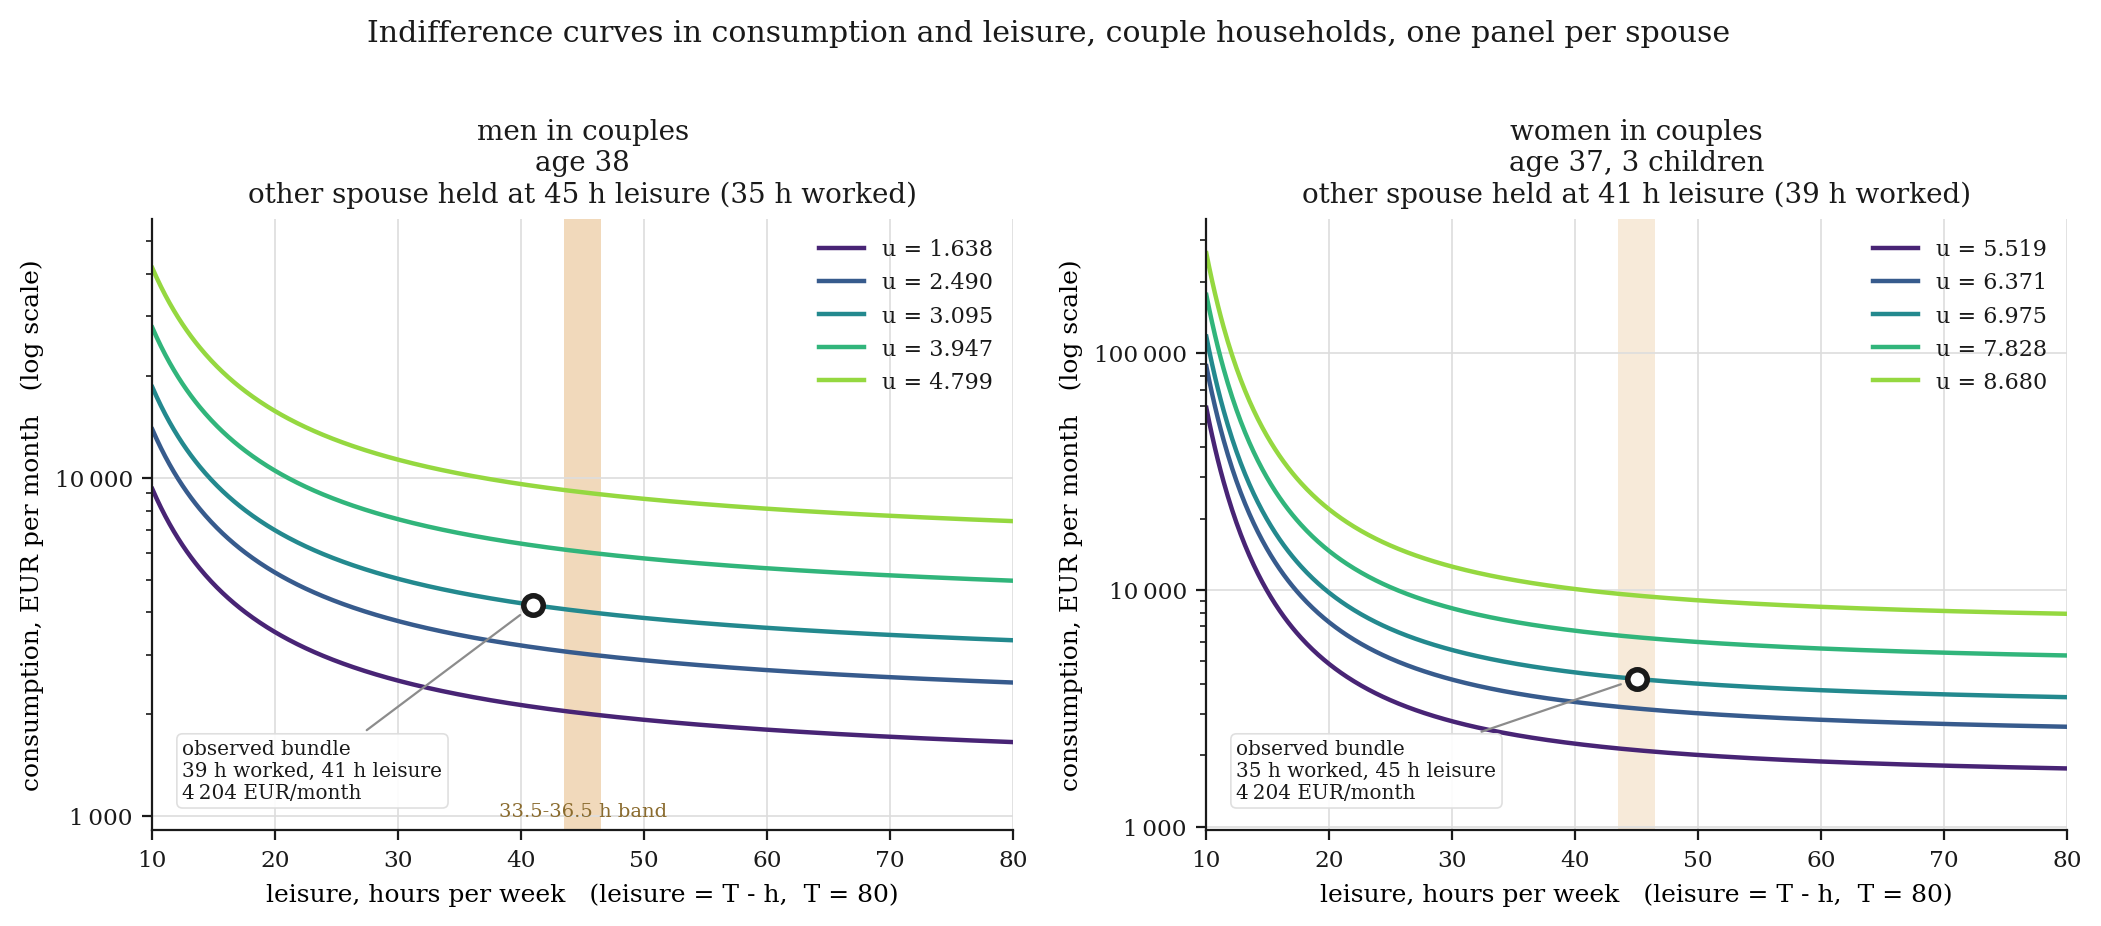
\includegraphics[width=0.95\linewidth,height=\textheight,keepaspectratio,alt={Indifference curves in consumption and each spouse's leisure, couple households, with the partner's leisure held at its observed value. Conditional slices of a joint object, not attainable sets.}]{figures/v5/figP02_indifference_curves_couples.png}
\caption{Indifference curves in consumption and each spouse's leisure, couple households, with the partner's leisure held at its observed value. Conditional slices of a joint object, not attainable sets.}
\end{figure}

\begin{figure}[H]
\centering
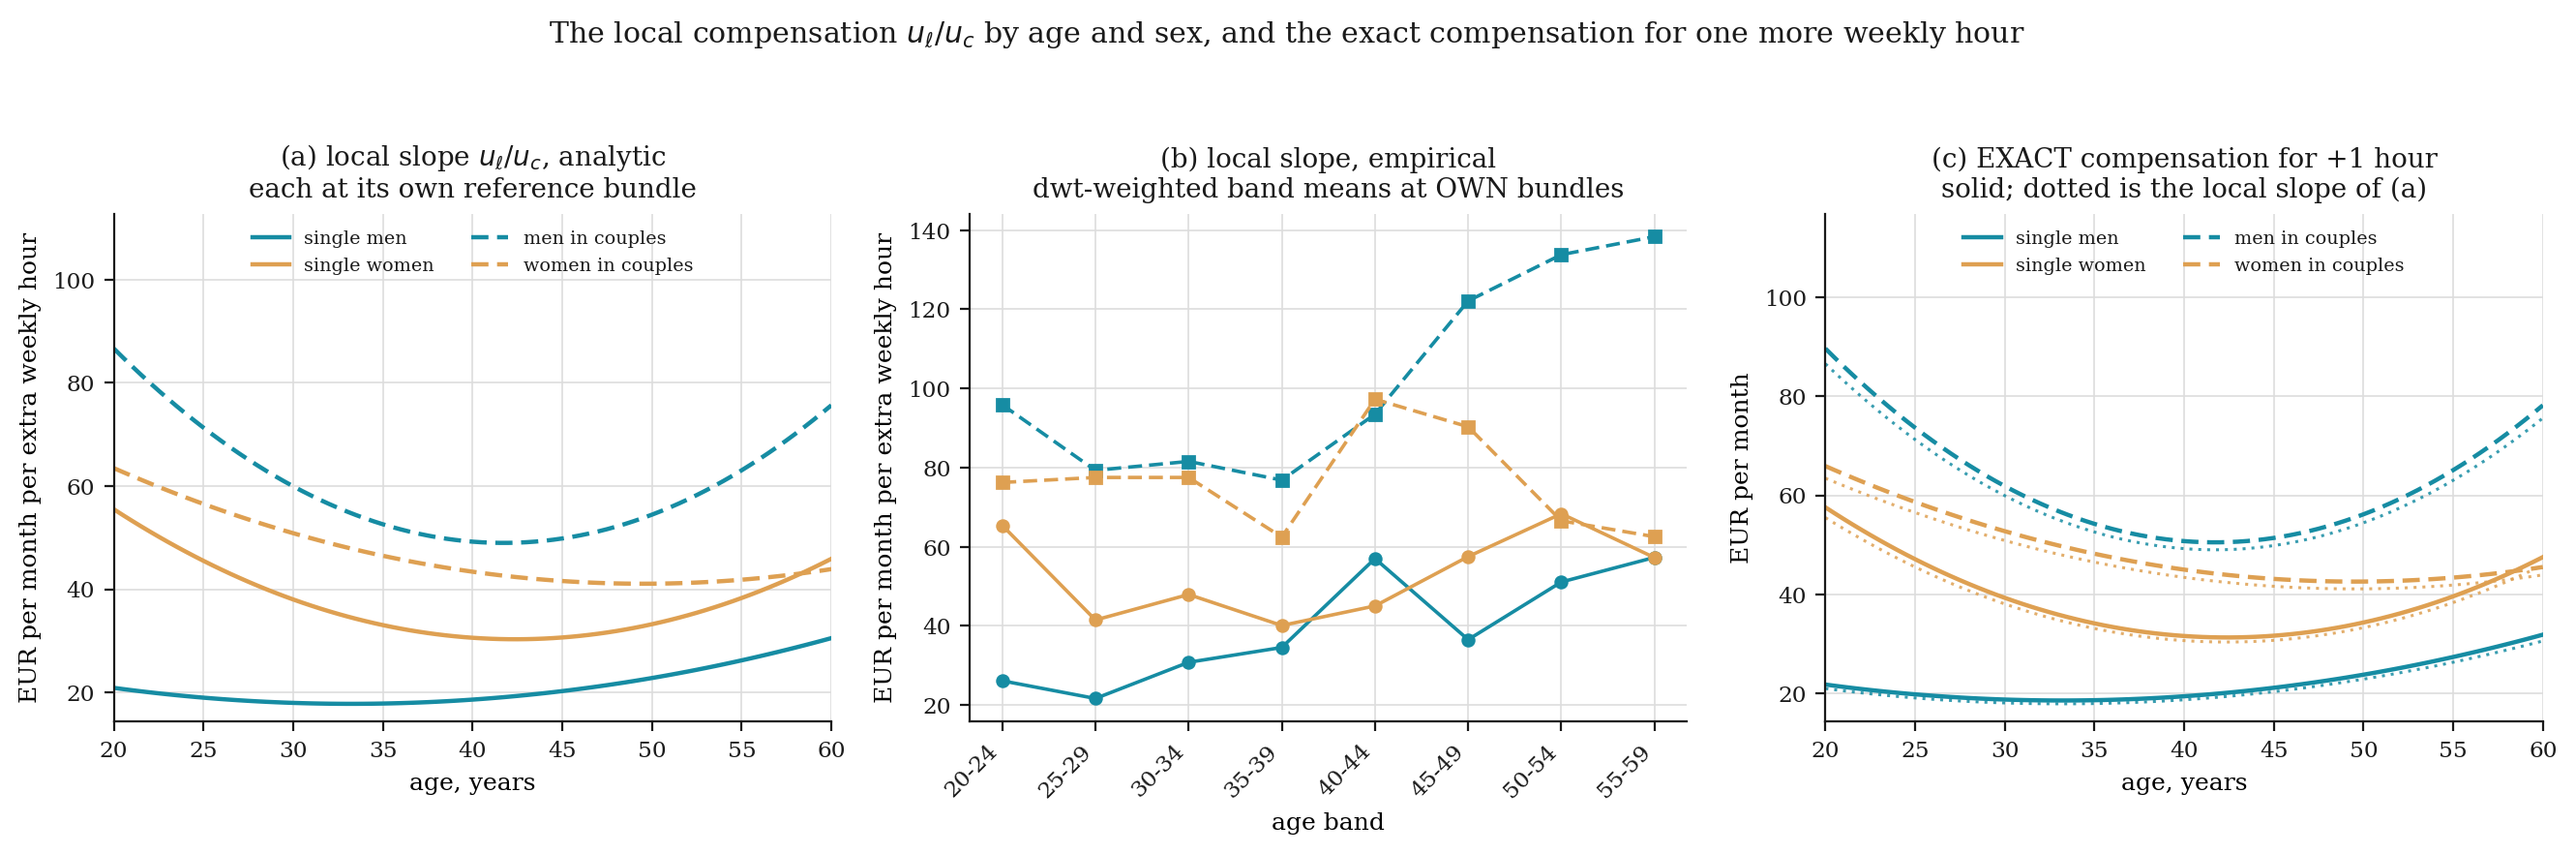
\includegraphics[width=0.95\linewidth,height=\textheight,keepaspectratio,alt={Marginal rate of substitution between leisure and consumption, by age and sex, in euros per month per additional recurring weekly hour of leisure. A compensation along an indifference curve, not a behavioural response to a wage change.}]{figures/v5/figP04_mrs_by_age_sex.png}
\caption{Marginal rate of substitution between leisure and consumption, by age and sex, in euros per month per additional recurring weekly hour of leisure. A compensation along an indifference curve, not a behavioural response to a wage change.}
\end{figure}

The indifference curves and the marginal rate of substitution are the economics; the coefficients are coordinates. Note that the consumption axis is logarithmic and the curves are drawn over the plotted range only: under \(L(\ell)+\beta_c\log(C/\lambda_c)\), any finite utility target at positive leisure is reached at the finite positive consumption \(C=\lambda_c\exp\{(\bar u-L(\ell))/\beta_c\}\), which is strictly positive for every finite target. A curve leaving the frame has left the plotting range, not the domain of the model, and nothing here is economically infeasible.


\subsection{Fit}\label{fit}

The fit reported here is a population prediction, computed by integrating the estimated model over the opportunity distribution and the taste shocks. It is not a sampled-menu choice probability and it is not an in-sample fitted value. We report it band-referenced: each group's weighted extensive-margin accuracy is compared not to a 100 per cent target -- a correctly specified stochastic-choice model does not attain one -- but to the 95 per cent band that model itself would produce by chance, from 500 outcome vectors simulated at the fitted estimates.

\begin{figure}[H]
\centering
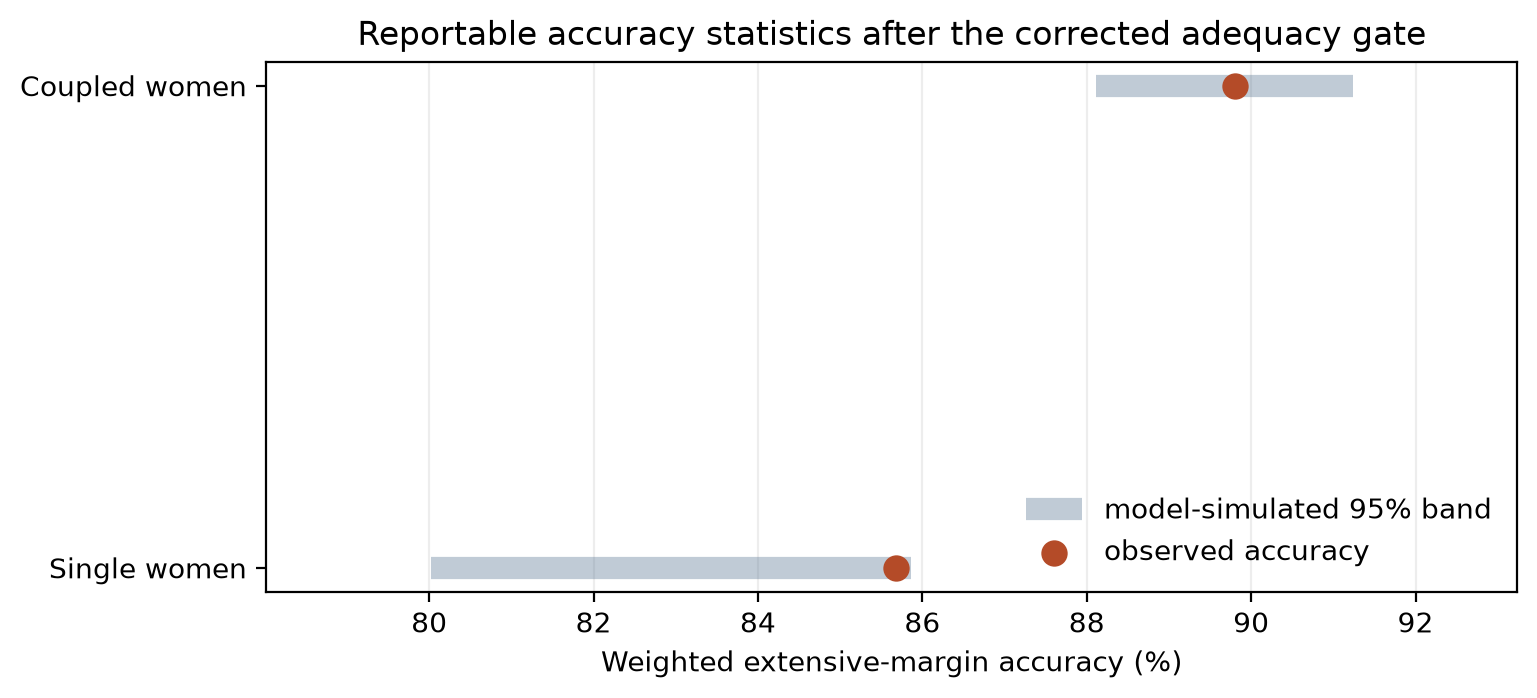
\includegraphics[width=0.95\linewidth,height=\textheight,keepaspectratio,alt={Corrected weighted extensive accuracy. Only single women and coupled women clear the preregistered numerical-adequacy gate. The statistics for single men and coupled men are quadrature-limited and withheld. Source: POSFIT v3b.}]{figures/v7/fitext_band_v3b.png}
\caption{\textbf{Corrected weighted extensive accuracy.} Only single women and coupled women clear the preregistered numerical-adequacy gate. The statistics for single men and coupled men are quadrature-limited and withheld. Source: POSFIT v3b.}
\end{figure}

\begin{figure}[H]
\centering
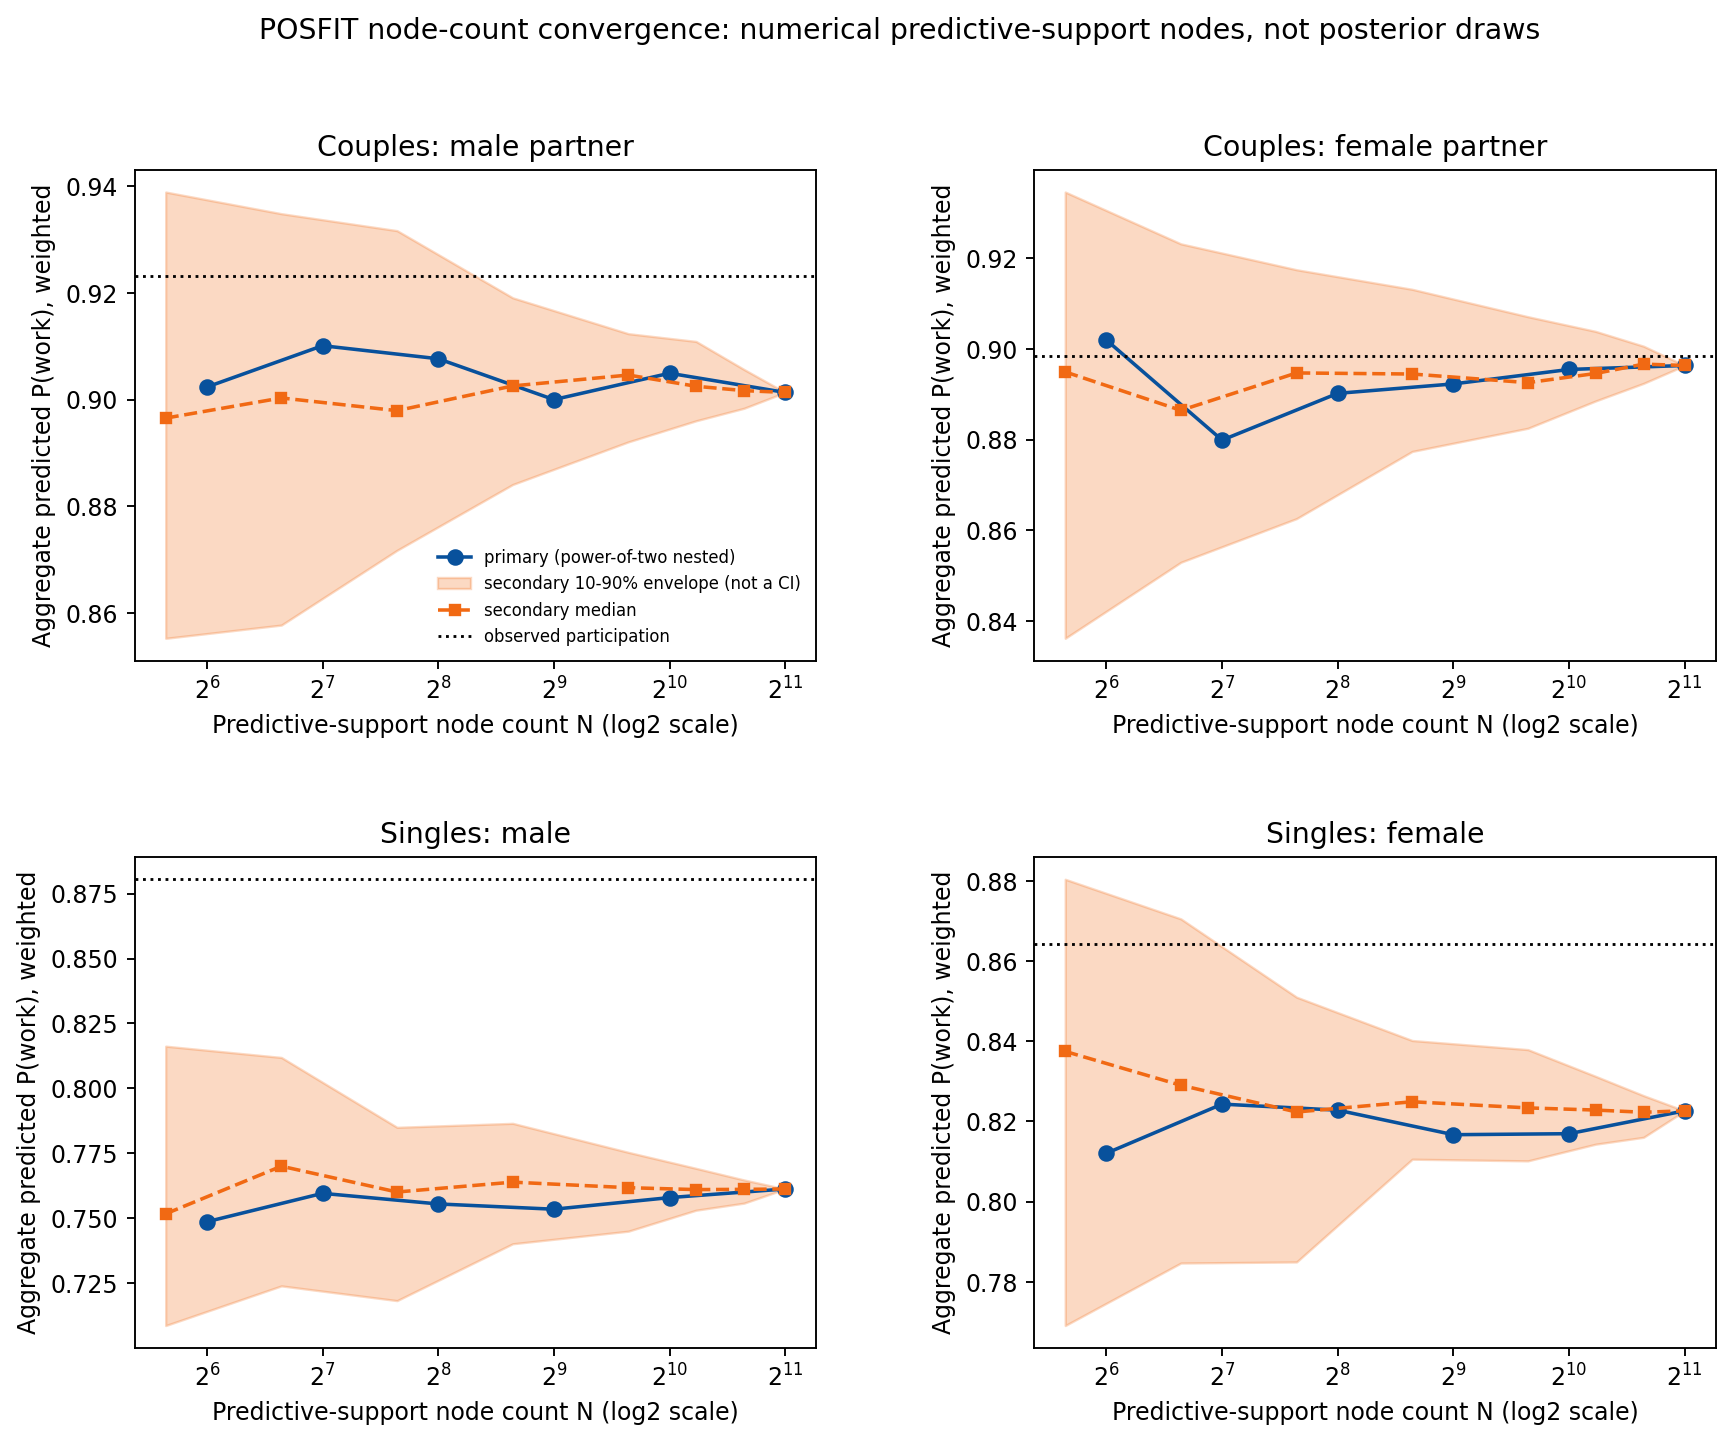
\includegraphics[width=0.95\linewidth,height=\textheight,keepaspectratio,alt={Corrected predictive/integration-node convergence. Weighted predicted participation over fixed-seed node subsets; the shaded area is the numerical 10--90\% envelope and observed participation is the horizontal reference. Source: POSFIT node convergence v3b.}]{figures/v7/node_convergence_v3b.png}
\caption{\textbf{Corrected predictive/integration-node convergence.} Weighted predicted participation over fixed-seed node subsets; the shaded area is the numerical 10--90\% envelope and observed participation is the horizontal reference. Source: POSFIT node convergence v3b.}
\end{figure}

The full reader surface -- all four extensive matrices and four joint hours-state matrices, the four worker-conditional intensive matrices with per-bin statistics, raw counts beside survey-weighted companions, observed-state probability, Brier and log scores, calibration, and the model-simulated benchmark -- is retained in the canonical notebook and results gallery. This report keeps the presentation concise and does not add a group-level fit claim.

Population participation and occupation margins remain close in aggregate, while the corrected hours comparison is uneven. The corrected individual-level diagnostics are adjudicated group by group below; no cross-group excess-predictability headline is maintained.

The corrected POSFIT-v3b numerical-adequacy gate is applied mechanically at the preregistered 0.25 threshold. Single women (85.7\%, simulated 95\% band {[}80.0\%, 85.9\%{]}, ratio 0.096) and coupled women (89.8\%, {[}88.1\%, 91.2\%{]}, ratio 0.049) clear it and are reportable. Single men (ratio 0.361) and coupled men (ratio 0.353) are quadrature-limited, so their extensive accuracy is withheld. In particular, coupled men crossed the threshold after the corrected S11 evaluation and the earlier reportable classification is not preserved.

\subsubsection{The full margin-by-margin comparison}\label{the-full-margin-by-margin-comparison}

\begin{figure}[H]
\centering
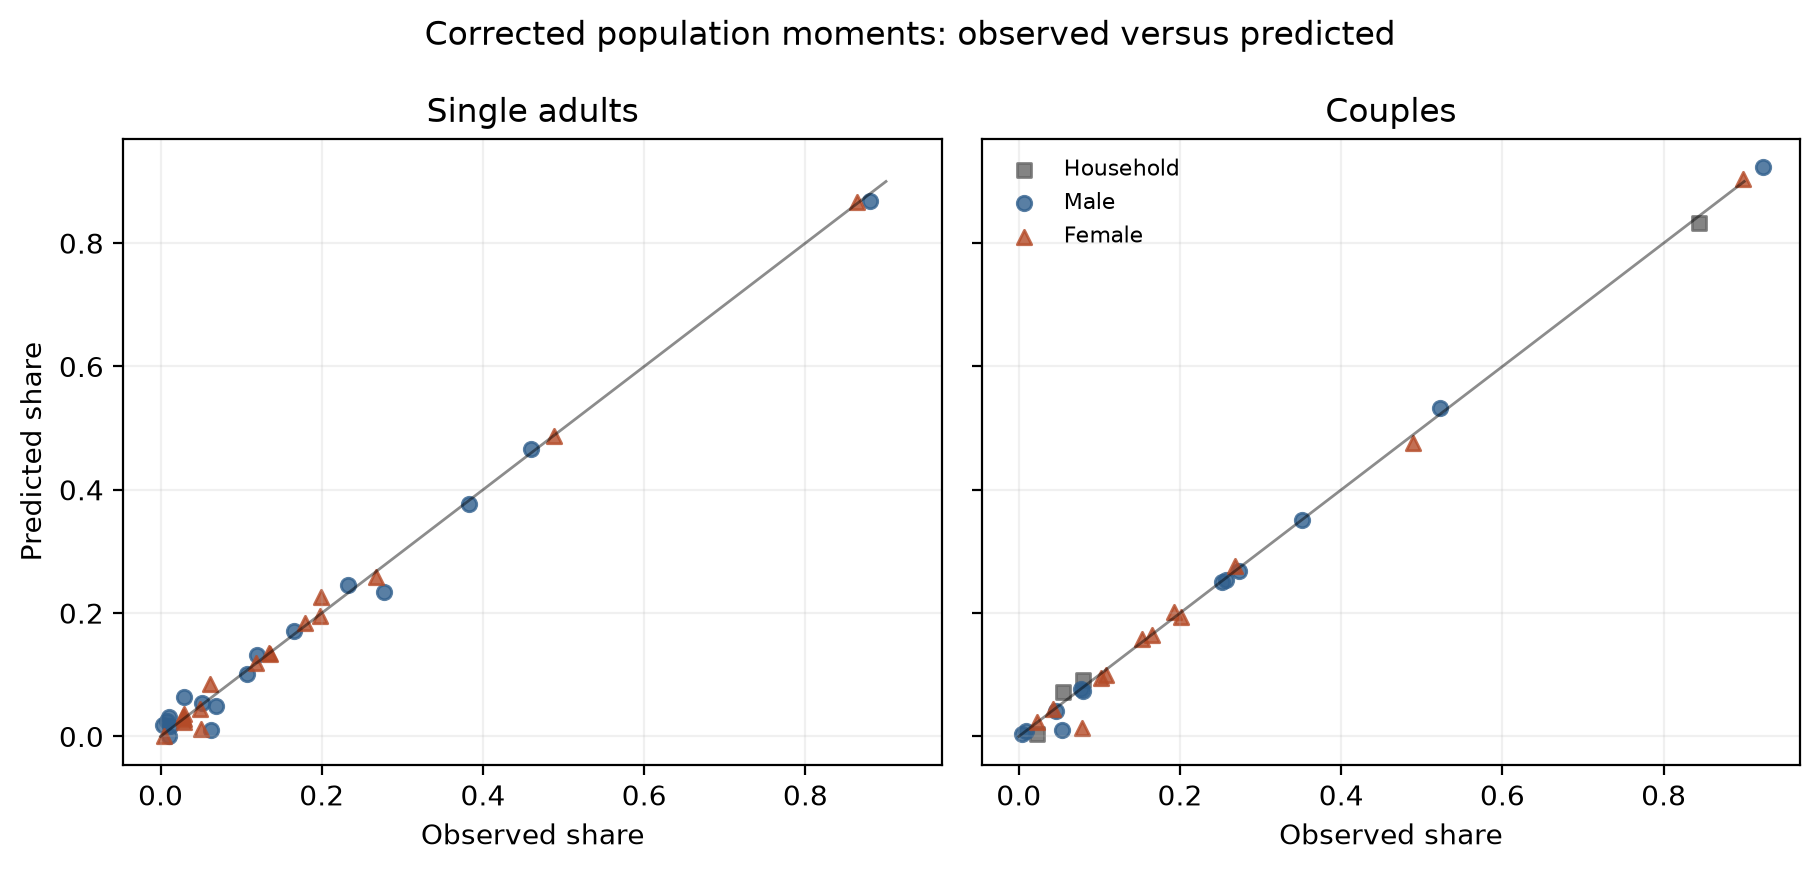
\includegraphics[width=0.95\linewidth,height=\textheight,keepaspectratio,alt={Corrected population fit. Observed against fully re-evaluated S11 model shares using S11/S10 structural-band indicators. The observed 37-hour mass-point cell is a descriptive residual category outside structural FT.}]{figures/v7/fit_by_margin_v7.png}
\caption{\textbf{Corrected population fit.} Observed against fully re-evaluated S11 model shares using S11/S10 structural-band indicators. The observed 37-hour mass-point cell is a descriptive residual category outside structural FT.}
\end{figure}

\Needspace*{12\baselineskip}\small\setlength{\tabcolsep}{3pt}\begin{longtable}[]{@{}
  >{\raggedright\arraybackslash}p{(\linewidth - 10\tabcolsep) * \real{0.1667}}
  >{\raggedright\arraybackslash}p{(\linewidth - 10\tabcolsep) * \real{0.1667}}
  >{\raggedright\arraybackslash}p{(\linewidth - 10\tabcolsep) * \real{0.1667}}
  >{\raggedright\arraybackslash}p{(\linewidth - 10\tabcolsep) * \real{0.1667}}
  >{\raggedright\arraybackslash}p{(\linewidth - 10\tabcolsep) * \real{0.1667}}
  >{\raggedright\arraybackslash}p{(\linewidth - 10\tabcolsep) * \real{0.1667}}@{}}
\caption{Corrected observed against model population moments, singles. Structural PT1, PT2 and FT rows use the S11/S10 definitions; the other hours rows are mutually exclusive descriptive residual categories, including the observed 37-hour mass-point cell. Predictions were fully re-evaluated after rebuilding the structural indicators; no row is a relabelling of the superseded evaluation.}\tabularnewline
\toprule\noalign{}
\begin{minipage}[b]{\linewidth}\raggedright
Unit
\end{minipage} & \begin{minipage}[b]{\linewidth}\raggedright
Moment
\end{minipage} & \begin{minipage}[b]{\linewidth}\raggedright
Observed
\end{minipage} & \begin{minipage}[b]{\linewidth}\raggedright
Model
\end{minipage} & \begin{minipage}[b]{\linewidth}\raggedright
Absolute deviation
\end{minipage} & \begin{minipage}[b]{\linewidth}\raggedright
Denominator
\end{minipage} \\
\midrule\noalign{}
\endfirsthead
\toprule\noalign{}
\begin{minipage}[b]{\linewidth}\raggedright
Unit
\end{minipage} & \begin{minipage}[b]{\linewidth}\raggedright
Moment
\end{minipage} & \begin{minipage}[b]{\linewidth}\raggedright
Observed
\end{minipage} & \begin{minipage}[b]{\linewidth}\raggedright
Model
\end{minipage} & \begin{minipage}[b]{\linewidth}\raggedright
Absolute deviation
\end{minipage} & \begin{minipage}[b]{\linewidth}\raggedright
Denominator
\end{minipage} \\
\midrule\noalign{}
\endhead
\bottomrule\noalign{}
\endlastfoot
Man & Employment & 0.8805 & 0.8675 & 0.0130 & households \\
Man & Hours: non-employment & 0.1195 & 0.1325 & 0.0130 & households \\
Man & Hours: {[}5, 10) & 0.0109 & 0.0000 & 0.0109 & households \\
Man & Hours: {[}10, 18.5) & 0.0080 & 0.0246 & 0.0166 & households \\
Man & Structural PT1: {[}18.5, 21.5) & 0.0113 & 0.0167 & 0.0054 & households \\
Man & Hours: {[}21.5, 29.5) & 0.0286 & 0.0646 & 0.0360 & households \\
Man & Structural PT2: {[}29.5, 30.5) & 0.0032 & 0.0187 & 0.0155 & households \\
Man & Hours: {[}30.5, 33.5) & 0.0107 & 0.0315 & 0.0208 & households \\
Man & Hours: {[}33.5, 36.5) & 0.2329 & 0.2457 & 0.0128 & households \\
Man & Observed 37-hour mass point: {[}36.5, 37.5) & 0.0624 & 0.0105 & 0.0519 & households \\
Man & Structural FT: {[}37.5, 40.5{]} & 0.2776 & 0.2347 & 0.0429 & households \\
Man & Hours: (40.5, 44.5) & 0.0691 & 0.0488 & 0.0203 & households \\
Man & Hours: {[}44.5, 70{]} & 0.1658 & 0.1717 & 0.0059 & households \\
Man & Occupation group 1 & 0.3823 & 0.3774 & 0.0049 & workers \\
Man & Occupation group 2 & 0.1069 & 0.1014 & 0.0054 & workers \\
Man & Occupation group 3 & 0.0516 & 0.0545 & 0.0029 & workers \\
Man & Occupation group 4 & 0.4593 & 0.4667 & 0.0074 & workers \\
Man & Mean log wage & 2.6876 & 2.6309 & 0.0567 & workers \\
Woman & Employment & 0.8642 & 0.8665 & 0.0024 & households \\
Woman & Hours: non-employment & 0.1358 & 0.1335 & 0.0024 & households \\
Woman & Hours: {[}5, 10) & 0.0042 & 0.0000 & 0.0042 & households \\
Woman & Hours: {[}10, 18.5) & 0.0278 & 0.0317 & 0.0038 & households \\
Woman & Structural PT1: {[}18.5, 21.5) & 0.0290 & 0.0283 & 0.0007 & households \\
Woman & Hours: {[}21.5, 29.5) & 0.0612 & 0.0856 & 0.0245 & households \\
Woman & Structural PT2: {[}29.5, 30.5) & 0.0288 & 0.0236 & 0.0052 & households \\
Woman & Hours: {[}30.5, 33.5) & 0.0290 & 0.0367 & 0.0077 & households \\
Woman & Hours: {[}33.5, 36.5) & 0.2672 & 0.2581 & 0.0091 & households \\
Woman & Observed 37-hour mass point: {[}36.5, 37.5) & 0.0503 & 0.0123 & 0.0381 & households \\
Woman & Structural FT: {[}37.5, 40.5{]} & 0.1990 & 0.2264 & 0.0274 & households \\
Woman & Hours: (40.5, 44.5) & 0.0492 & 0.0446 & 0.0045 & households \\
Woman & Hours: {[}44.5, 70{]} & 0.1185 & 0.1192 & 0.0007 & households \\
Woman & Occupation group 1 & 0.1795 & 0.1832 & 0.0036 & workers \\
Woman & Occupation group 2 & 0.1976 & 0.1946 & 0.0031 & workers \\
Woman & Occupation group 3 & 0.1349 & 0.1348 & 0.0002 & workers \\
Woman & Occupation group 4 & 0.4879 & 0.4875 & 0.0004 & workers \\
Woman & Mean log wage & 2.5968 & 2.6207 & 0.0238 & workers \\
\end{longtable}

\Needspace*{12\baselineskip}\small\setlength{\tabcolsep}{3pt}\begin{longtable}[]{@{}
  >{\raggedright\arraybackslash}p{(\linewidth - 10\tabcolsep) * \real{0.1667}}
  >{\raggedright\arraybackslash}p{(\linewidth - 10\tabcolsep) * \real{0.1667}}
  >{\raggedright\arraybackslash}p{(\linewidth - 10\tabcolsep) * \real{0.1667}}
  >{\raggedright\arraybackslash}p{(\linewidth - 10\tabcolsep) * \real{0.1667}}
  >{\raggedright\arraybackslash}p{(\linewidth - 10\tabcolsep) * \real{0.1667}}
  >{\raggedright\arraybackslash}p{(\linewidth - 10\tabcolsep) * \real{0.1667}}@{}}
\caption{Corrected observed against model population moments, couples. Structural PT1, PT2 and FT rows use the S11/S10 definitions; the other hours rows are mutually exclusive descriptive residual categories, including the observed 37-hour mass-point cell. Predictions were fully re-evaluated after rebuilding the structural indicators; no row is a relabelling of the superseded evaluation.}\tabularnewline
\toprule\noalign{}
\begin{minipage}[b]{\linewidth}\raggedright
Unit
\end{minipage} & \begin{minipage}[b]{\linewidth}\raggedright
Moment
\end{minipage} & \begin{minipage}[b]{\linewidth}\raggedright
Observed
\end{minipage} & \begin{minipage}[b]{\linewidth}\raggedright
Model
\end{minipage} & \begin{minipage}[b]{\linewidth}\raggedright
Absolute deviation
\end{minipage} & \begin{minipage}[b]{\linewidth}\raggedright
Denominator
\end{minipage} \\
\midrule\noalign{}
\endfirsthead
\toprule\noalign{}
\begin{minipage}[b]{\linewidth}\raggedright
Unit
\end{minipage} & \begin{minipage}[b]{\linewidth}\raggedright
Moment
\end{minipage} & \begin{minipage}[b]{\linewidth}\raggedright
Observed
\end{minipage} & \begin{minipage}[b]{\linewidth}\raggedright
Model
\end{minipage} & \begin{minipage}[b]{\linewidth}\raggedright
Absolute deviation
\end{minipage} & \begin{minipage}[b]{\linewidth}\raggedright
Denominator
\end{minipage} \\
\midrule\noalign{}
\endhead
\bottomrule\noalign{}
\endlastfoot
Household & Joint regime neither works & 0.0222 & 0.0043 & 0.0178 & households \\
Household & Joint regime man only & 0.0794 & 0.0909 & 0.0115 & households \\
Household & Joint regime woman only & 0.0547 & 0.0723 & 0.0176 & households \\
Household & Joint regime both work & 0.8437 & 0.8324 & 0.0113 & households \\
Man & Employment & 0.9231 & 0.9234 & 0.0002 & households \\
Man & Hours: non-employment & 0.0769 & 0.0766 & 0.0002 & households \\
Man & Structural PT1: {[}18.5, 21.5) & 0.0037 & 0.0041 & 0.0004 & households \\
Man & Structural PT2: {[}29.5, 30.5) & 0.0093 & 0.0094 & 0.0002 & households \\
Man & Hours: {[}33.5, 36.5) & 0.2515 & 0.2507 & 0.0008 & households \\
Man & Observed 37-hour mass point: {[}36.5, 37.5) & 0.0539 & 0.0098 & 0.0441 & households \\
Man & Structural FT: {[}37.5, 40.5{]} & 0.2736 & 0.2682 & 0.0054 & households \\
Man & Hours: {[}44.5, 70{]} & 0.2576 & 0.2531 & 0.0044 & households \\
Man & Occupation group 1 & 0.3519 & 0.3516 & 0.0003 & workers \\
Man & Occupation group 2 & 0.0797 & 0.0741 & 0.0056 & workers \\
Man & Occupation group 3 & 0.0464 & 0.0412 & 0.0052 & workers \\
Man & Occupation group 4 & 0.5220 & 0.5331 & 0.0111 & workers \\
Man & Mean log wage & 2.7687 & 2.7054 & 0.0633 & workers \\
Woman & Employment & 0.8984 & 0.9047 & 0.0063 & households \\
Woman & Hours: non-employment & 0.1016 & 0.0953 & 0.0063 & households \\
Woman & Structural PT1: {[}18.5, 21.5) & 0.0229 & 0.0230 & 0.0001 & households \\
Woman & Structural PT2: {[}29.5, 30.5) & 0.0419 & 0.0439 & 0.0020 & households \\
Woman & Hours: {[}33.5, 36.5) & 0.2687 & 0.2767 & 0.0080 & households \\
Woman & Observed 37-hour mass point: {[}36.5, 37.5) & 0.0785 & 0.0134 & 0.0651 & households \\
Woman & Structural FT: {[}37.5, 40.5{]} & 0.2008 & 0.1938 & 0.0070 & households \\
Woman & Hours: {[}44.5, 70{]} & 0.1079 & 0.1002 & 0.0077 & households \\
Woman & Occupation group 1 & 0.1653 & 0.1648 & 0.0005 & workers \\
Woman & Occupation group 2 & 0.1922 & 0.2017 & 0.0095 & workers \\
Woman & Occupation group 3 & 0.1533 & 0.1583 & 0.0050 & workers \\
Woman & Occupation group 4 & 0.4892 & 0.4752 & 0.0140 & workers \\
Woman & Mean log wage & 2.6072 & 2.6319 & 0.0247 & workers \\
\end{longtable}

The corrected mean absolute deviation over all population moments is 0.0140 across 36 single-adult moments and 0.0119 across 30 couple moments. This correction is not an across-the-board fit improvement: singles MAE rises slightly, while couples MAE falls. The remaining common mismatch is underprediction of the observed 37-hour mass point, by 3.8--6.5 percentage points across the four groups. That mass point lies outside the S11 structural full-time band \([37.5,40.5]\); it is not described as underprediction of that structural band. The sub-ten-hour cell remains a finite-integration-panel coverage limitation, and the long-hours reporting bin closes at 70 inclusive.

\Needspace*{12\baselineskip}\small\setlength{\tabcolsep}{3pt}\begin{longtable}[]{@{}
  >{\raggedright\arraybackslash}p{(\linewidth - 8\tabcolsep) * \real{0.2000}}
  >{\raggedright\arraybackslash}p{(\linewidth - 8\tabcolsep) * \real{0.2000}}
  >{\raggedright\arraybackslash}p{(\linewidth - 8\tabcolsep) * \real{0.2000}}
  >{\raggedright\arraybackslash}p{(\linewidth - 8\tabcolsep) * \real{0.2000}}
  >{\raggedright\arraybackslash}p{(\linewidth - 8\tabcolsep) * \real{0.2000}}@{}}
\caption{The estimated singles model against two re-estimated common-opportunity benchmarks. Estimates and maximized criteria are unchanged; criterion-B population moments are corrected to the S11/S10 structural-band definitions. The RUM-A estimation-input band defect and its cancellation in the conditional likelihood are disclosed in the limitations.}\tabularnewline
\toprule\noalign{}
\begin{minipage}[b]{\linewidth}\raggedright
Specification
\end{minipage} & \begin{minipage}[b]{\linewidth}\raggedright
Free coordinates
\end{minipage} & \begin{minipage}[b]{\linewidth}\raggedright
Criterion
\end{minipage} & \begin{minipage}[b]{\linewidth}\raggedright
Difference
\end{minipage} & \begin{minipage}[b]{\linewidth}\raggedright
Population fit
\end{minipage} \\
\midrule\noalign{}
\endfirsthead
\toprule\noalign{}
\begin{minipage}[b]{\linewidth}\raggedright
Specification
\end{minipage} & \begin{minipage}[b]{\linewidth}\raggedright
Free coordinates
\end{minipage} & \begin{minipage}[b]{\linewidth}\raggedright
Criterion
\end{minipage} & \begin{minipage}[b]{\linewidth}\raggedright
Difference
\end{minipage} & \begin{minipage}[b]{\linewidth}\raggedright
Population fit
\end{minipage} \\
\midrule\noalign{}
\endhead
\bottomrule\noalign{}
\endlastfoot
Latent jobs with household-specific opportunities & 41 & 6253.463 & -- & 0.0140 \\
Benchmark A: common opportunity distribution, preferences re-estimated & 10 & 6403.974 & +150.51 & 0.0273 \\
Benchmark B: common opportunity shape, employment and hours moved into utility & 16 & 6395.108 & +141.64 & 0.0264 \\
\end{longtable}

The two re-estimated common-opportunity benchmarks are worse by 141.64 and by a larger margin, on the same households, the same sampled alternatives and the same criterion. The comparison is a nested one in the sense that the benchmarks restrict the opportunity block and re-estimate everything else, but we do not convert it into a formal test, because the sampled-alternative criterion is not the likelihood of the observed data and the conditions for a likelihood-ratio distribution are not established here. What the table does support is that the deterioration is concentrated where the opportunity block does its work: the population fit worsens from 0.0140 to 0.0273 and 0.0264, and the occupation margins deteriorate by an order of magnitude, from about half a percentage point to eleven. A better criterion does not by itself establish that a mechanism has been identified.


\subsection{Money-metric well-being}\label{money-metric-well-being}

\Needspace*{12\baselineskip}\small\setlength{\tabcolsep}{3pt}\begin{longtable}[]{@{}>{\RaggedRight\arraybackslash}p{0.1550\linewidth}>{\RaggedRight\arraybackslash}p{0.1212\linewidth}>{\RaggedRight\arraybackslash}p{0.1212\linewidth}>{\RaggedRight\arraybackslash}p{0.1212\linewidth}>{\RaggedRight\arraybackslash}p{0.1212\linewidth}>{\RaggedRight\arraybackslash}p{0.1212\linewidth}>{\RaggedRight\arraybackslash}p{0.1212\linewidth}@{}}
\caption{The distribution of money-metric well-being, and the priced disposable income it replaces. Levels are in euros per month of equivalent flat consumption, weighted. Levels are not comparable between the two household types: each type carries its own reference construction, and the Gini of the money metric and the Gini of income are not two estimates of one quantity.}\tabularnewline
\toprule\noalign{}
Population & Basis & Mean & p10 & Median & p90 & Gini \\
\midrule\noalign{}
\endfirsthead
\toprule\noalign{}
Population & Basis & Mean & p10 & Median & p90 & Gini \\
\midrule\noalign{}
\endhead
\bottomrule\noalign{}
\endlastfoot
Single-adult & Household & 4,354 & 2,643 & 4,139 & 6,219 & 0.1936 \\
Single-adult & Equivalized & 3,957 & 2,286 & 3,722 & 5,819 & 0.2089 \\
Single-adult & Priced disposable income & -- & -- & -- & -- & 0.2533 \\
Couple & Household & 1,839 & 1,353 & 1,767 & 2,326 & 0.1325 \\
Couple & Equivalized & 972 & 721 & 928 & 1,229 & 0.1274 \\
Couple & Priced disposable income & -- & -- & -- & -- & 0.2310 \\
\end{longtable}

\begin{figure}[H]
\centering
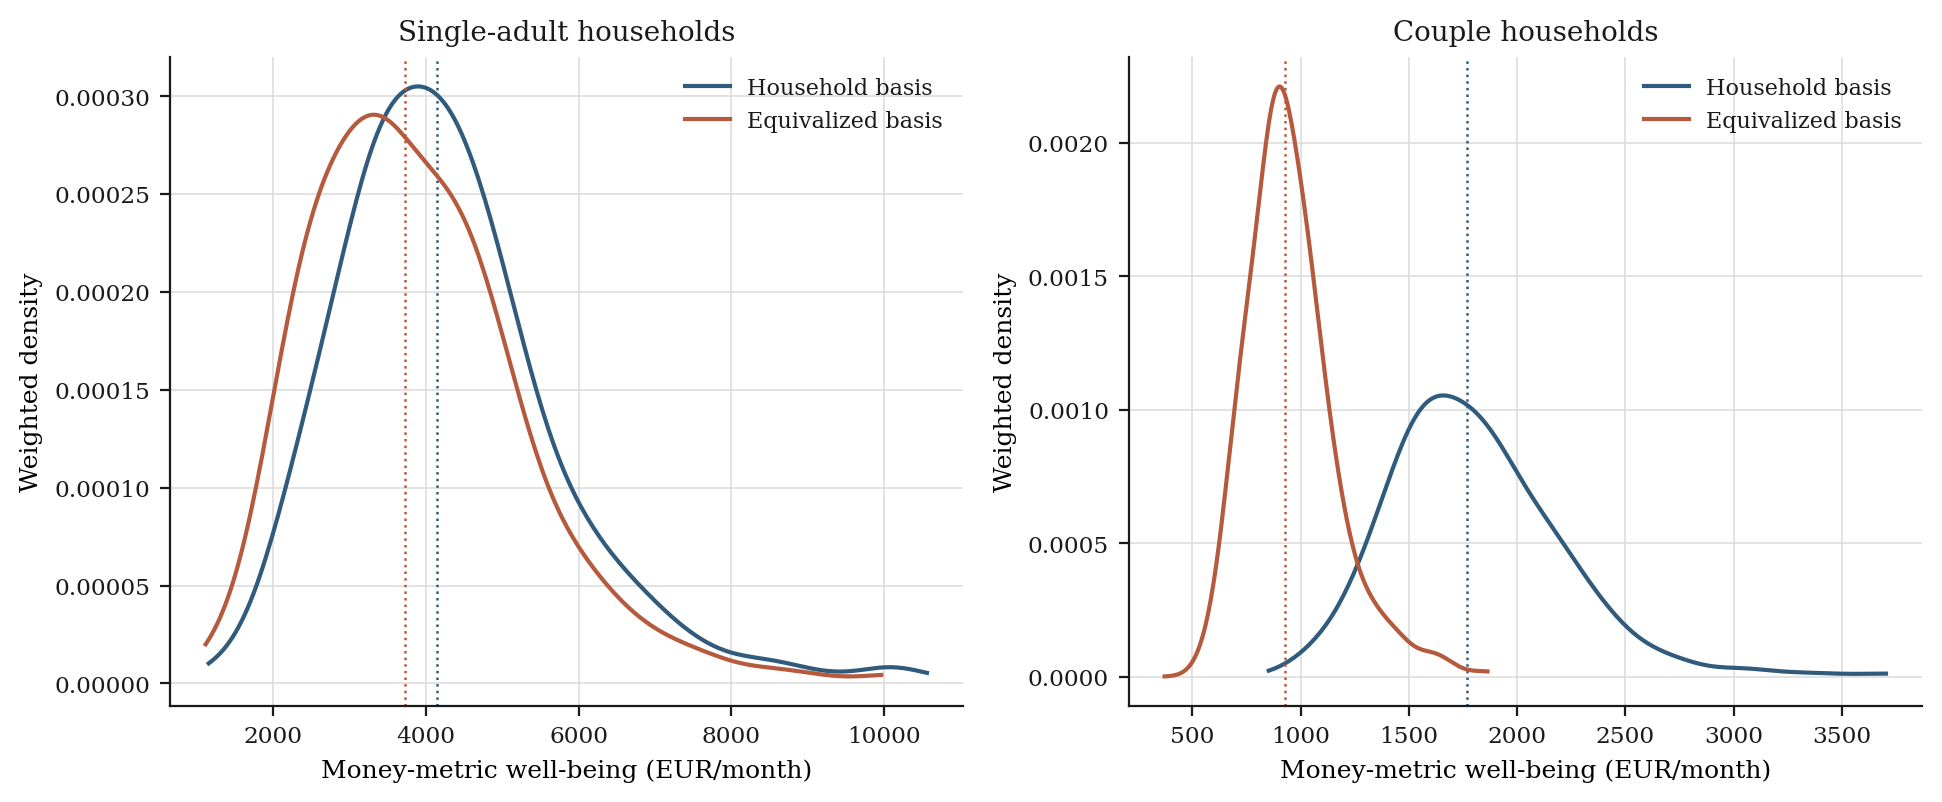
\includegraphics[width=0.95\linewidth,height=\textheight,keepaspectratio,alt={The distribution of money-metric well-being, by household type and basis, with weighted medians marked. Levels are not comparable across the two panels: each household type carries its own reference construction.}]{figures/v5/figV02_welfare_distributions.png}
\caption{The distribution of money-metric well-being, by household type and basis, with weighted medians marked. Levels are not comparable across the two panels: each household type carries its own reference construction.}
\end{figure}

\begin{figure}[H]
\centering
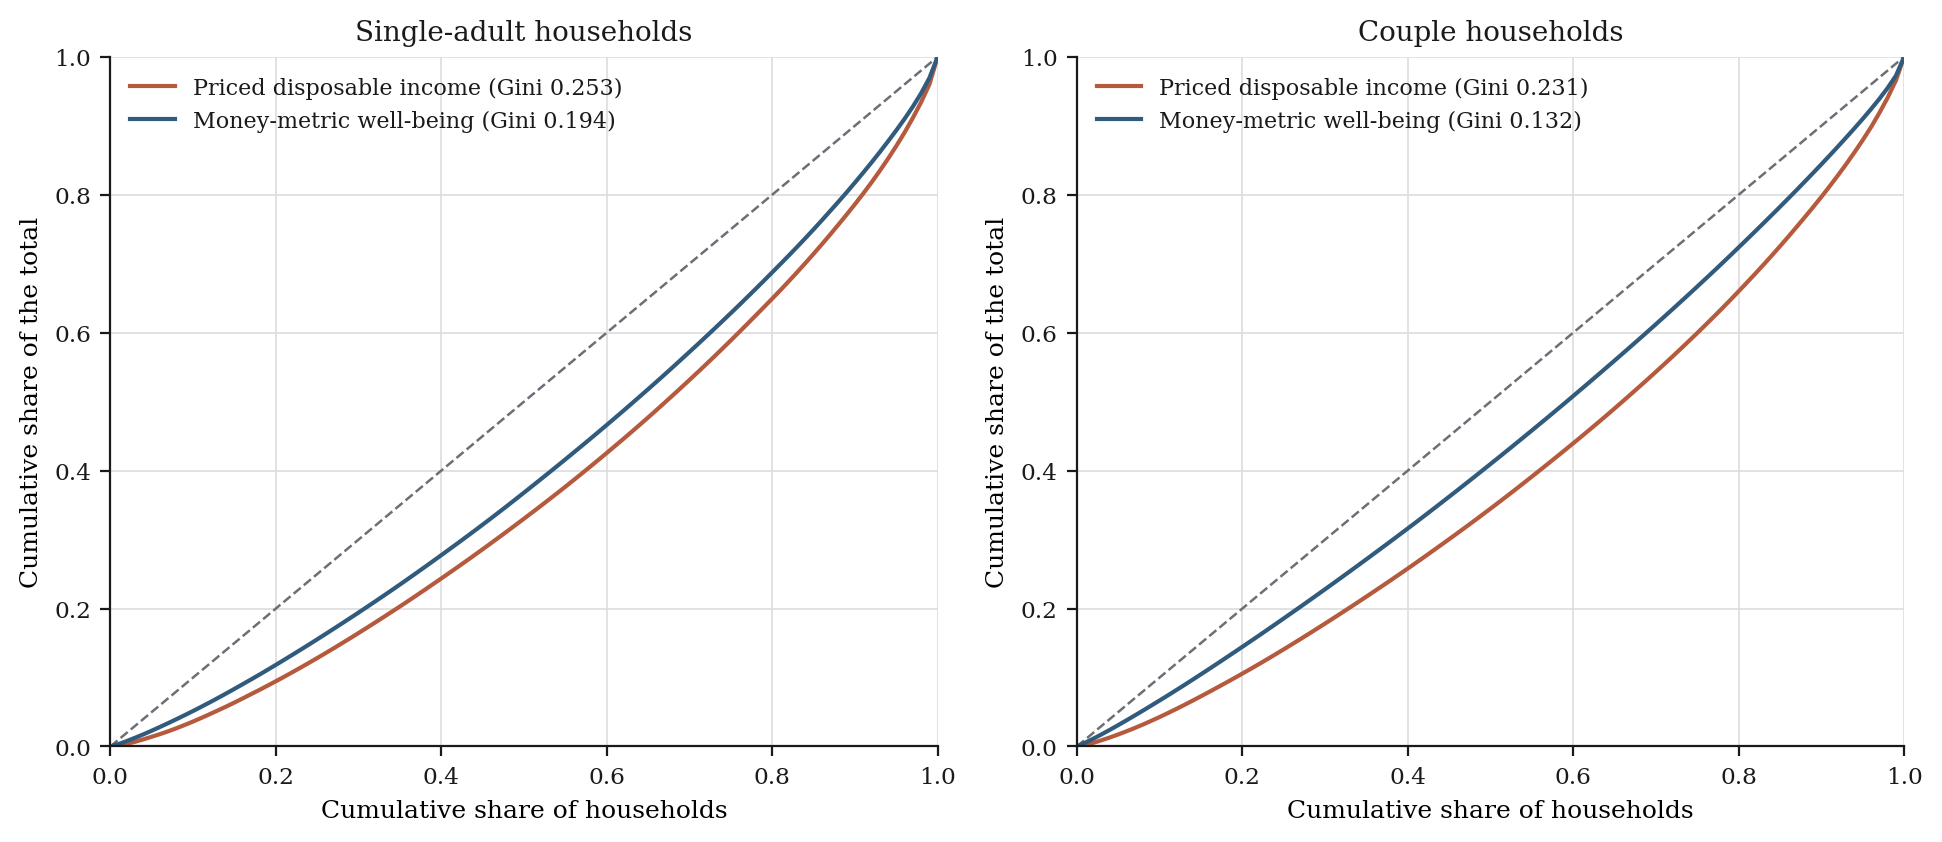
\includegraphics[width=0.95\linewidth,height=\textheight,keepaspectratio,alt={Lorenz curves of money-metric well-being and of the priced disposable income it replaces, over the same households and the same weights. The two curves answer different questions about the same households; their Gini values are not two estimates of one quantity.}]{figures/v5/figV01_welfare_lorenz.png}
\caption{Lorenz curves of money-metric well-being and of the priced disposable income it replaces, over the same households and the same weights. The two curves answer different questions about the same households; their Gini values are not two estimates of one quantity.}
\end{figure}

The money metric is less unequal than the priced disposable income it replaces, for both household types: the Gini falls from 0.253 to 0.194 for single adults and from 0.231 to 0.132 for couples. The two Ginis are not two estimates of one quantity. The income Gini describes an outcome; the welfare Gini describes an ex-ante monetary level built from each household's own preferences and own reachable jobs, and the difference between them is not a correction but a change of object.

Levels differ from income in opposite directions for the two types, and the levels are not comparable between them: each application carries its own reference construction, with a female-primary reference block for single adults and a medoid-spouse reference for couples, and the couples index adds two leisure terms. We use levels only within type and offer no mechanism for the between-type difference in levels.


\subsection{The decomposition}\label{the-decomposition}

\Needspace*{12\baselineskip}\small\setlength{\tabcolsep}{3pt}\begin{longtable}[]{@{}
  >{\raggedright\arraybackslash}p{(\linewidth - 4\tabcolsep) * \real{0.3333}}
  >{\raggedright\arraybackslash}p{(\linewidth - 4\tabcolsep) * \real{0.3333}}
  >{\raggedright\arraybackslash}p{(\linewidth - 4\tabcolsep) * \real{0.3333}}@{}}
\caption{The four coalition states of the two-group game and the corresponding one-factor effects. Weighted Gini of the money metric on the raw household basis, with the female-primary reference for single-adult households. The fully common state is zero to the precision reported in the text: that is a tested property of the game, not an imposed constraint. A positive percentage in the last two rows is a rise in inequality.}\tabularnewline
\toprule\noalign{}
\begin{minipage}[b]{\linewidth}\raggedright
State
\end{minipage} & \begin{minipage}[b]{\linewidth}\raggedright
Single-adult
\end{minipage} & \begin{minipage}[b]{\linewidth}\raggedright
Couple
\end{minipage} \\
\midrule\noalign{}
\endfirsthead
\toprule\noalign{}
\begin{minipage}[b]{\linewidth}\raggedright
State
\end{minipage} & \begin{minipage}[b]{\linewidth}\raggedright
Single-adult
\end{minipage} & \begin{minipage}[b]{\linewidth}\raggedright
Couple
\end{minipage} \\
\midrule\noalign{}
\endhead
\bottomrule\noalign{}
\endlastfoot
Own preferences, own circumstances & 0.193596 & 0.132465 \\
Common preferences, own circumstances & 0.218795 & 0.129046 \\
Own preferences, common circumstances & 0.063459 & 0.009427 \\
Common preferences, common circumstances & 0.000000 & 0.000000 \\
\emph{Preferences equalized alone: change in the Gini (per cent)} & +13.02 & -2.58 \\
\emph{All other circumstances equalized alone: change (per cent)} & -67.22 & -92.88 \\
\end{longtable}

The four states are the coalition values of the two-group game. Reading them directly gives the one-factor effects. For single adults, equalizing preferences alone \emph{raises} the Gini by 13.0 per cent, from 0.193596 to 0.218795; equalizing all non-preference circumstances alone lowers it by 67.2 per cent. For couples, equalizing preferences alone lowers the Gini by 2.6 per cent and equalizing all other circumstances lowers it by 92.9. The fully common state is zero to 1.3e-15 in index units, which is a tested property of the game and not an imposed constraint.

\begin{figure}[H]
\centering
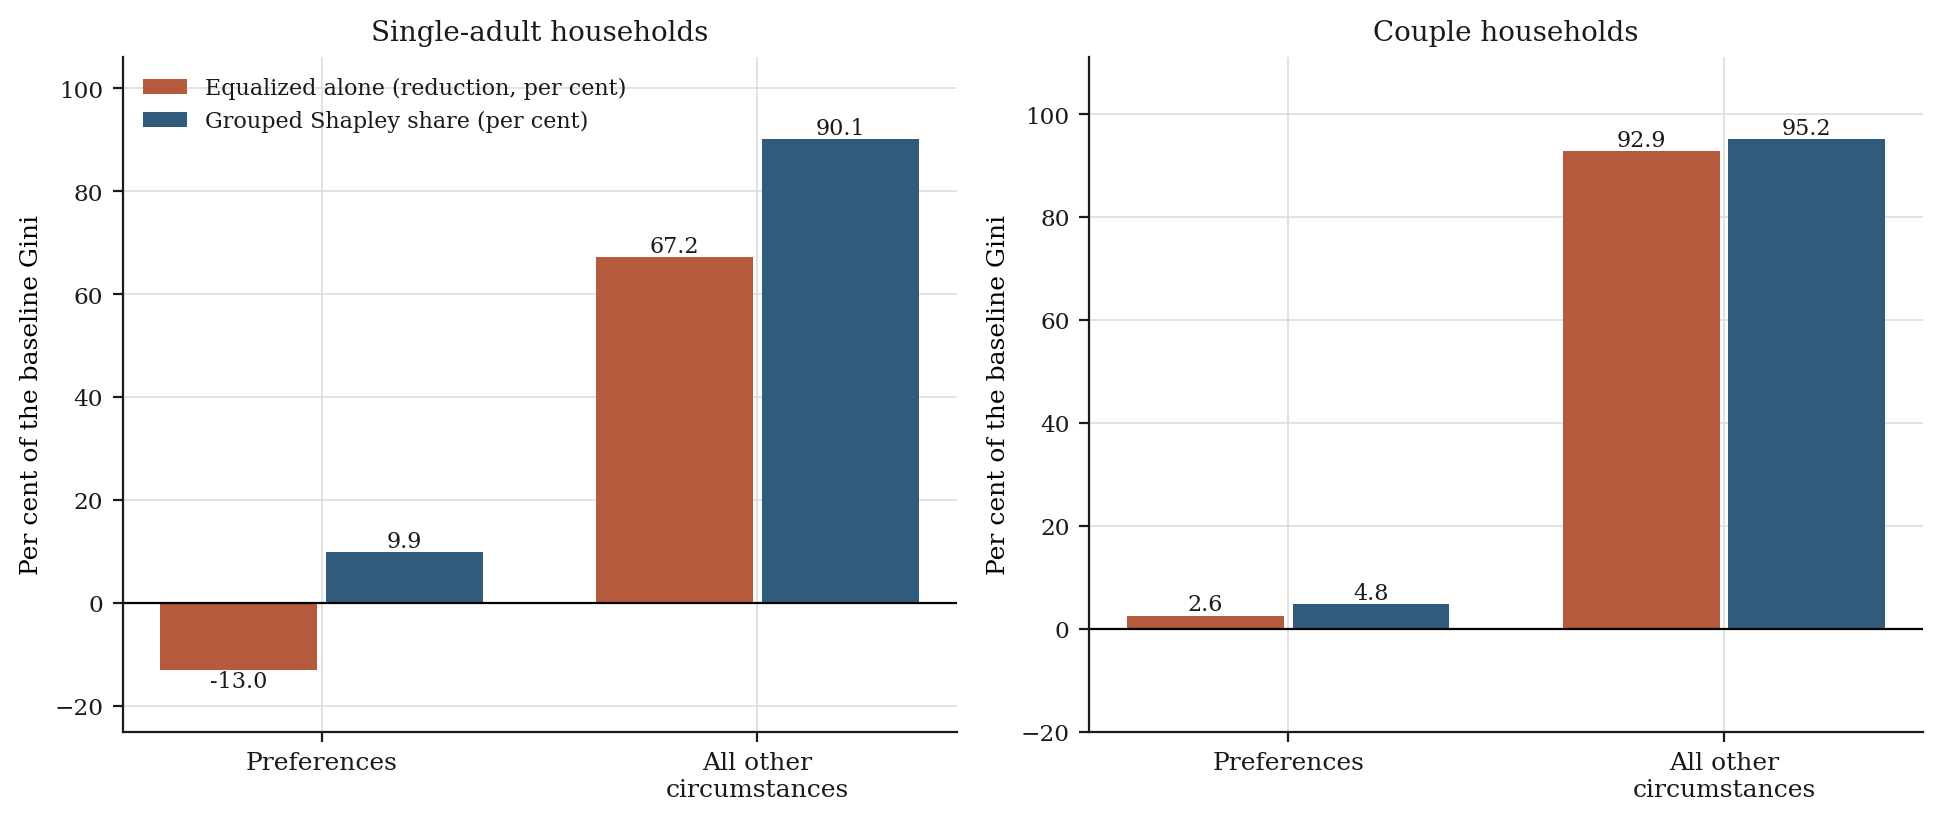
\includegraphics[width=0.95\linewidth,height=\textheight,keepaspectratio,alt={Equalizing one group alone against the grouped Shapley share. For single-adult households, equalizing preferences alone raises the Gini while the preference share is positive; the share averages marginal contributions over coalition orders and the one-factor effect does not.}]{figures/v5/figV04_one_factor_vs_shapley.png}
\caption{Equalizing one group alone against the grouped Shapley share. For single-adult households, equalizing preferences alone raises the Gini while the preference share is positive; the share averages marginal contributions over coalition orders and the one-factor effect does not.}
\end{figure}

The allocated shares are not those numbers. An allocated share is an average of marginal contributions over the orders in which coalitions can form; the one-factor effect is the contribution in exactly one order. For single adults the two even differ in sign, and the arithmetic of the game explains why. With four states and \(I_{11}=0\), the two-group closure gives

\[2\,C_P=I_{00}-I_{10}+I_{01}.\]

Since \(I_{01}\ge 0\) for a nonnegative index, a negative \(C_P\) forces \(I_{00}-I_{10}<0\), so a negative allocated share does imply that preference-only equalization raises inequality. The converse does not hold, and the single-adult Gini is the counterexample: \(C_P>0\) while \(I_{10}>I_{00}\). This is a consequence of the closure of \emph{this} exhaustive two-group game with a nonnegative index; it is not a general property of a Shapley allocation.

\Needspace*{12\baselineskip}\small\setlength{\tabcolsep}{3pt}\begin{longtable}[]{@{}
  >{\raggedright\arraybackslash}p{(\linewidth - 8\tabcolsep) * \real{0.2000}}
  >{\raggedright\arraybackslash}p{(\linewidth - 8\tabcolsep) * \real{0.2000}}
  >{\raggedright\arraybackslash}p{(\linewidth - 8\tabcolsep) * \real{0.2000}}
  >{\raggedright\arraybackslash}p{(\linewidth - 8\tabcolsep) * \real{0.2000}}
  >{\raggedright\arraybackslash}p{(\linewidth - 8\tabcolsep) * \real{0.2000}}@{}}
\caption{Grouped attribution of well-being inequality. Contributions in Gini points beside the share of the baseline Gini of the same population, per cent, with the 95 per cent cluster-robust parameter interval in brackets from 100 draws. Shares are taken against the baseline of the same population and are not comparable as levels across the two populations. The parameter interval and the RQMC integration band measure different things and are never combined; the integration band is reported separately in the text and in the figure. Resources and needs enter here as one component of the four-player game; its subdivision into non-labour resources and household composition is a nested attribution and has its own table.}\tabularnewline
\toprule\noalign{}
\begin{minipage}[b]{\linewidth}\raggedright
Component
\end{minipage} & \begin{minipage}[b]{\linewidth}\raggedright
Singles: Gini points
\end{minipage} & \begin{minipage}[b]{\linewidth}\raggedright
Singles: share {[}95 per cent{]}
\end{minipage} & \begin{minipage}[b]{\linewidth}\raggedright
Couples: Gini points
\end{minipage} & \begin{minipage}[b]{\linewidth}\raggedright
Couples: share {[}95 per cent{]}
\end{minipage} \\
\midrule\noalign{}
\endfirsthead
\toprule\noalign{}
\begin{minipage}[b]{\linewidth}\raggedright
Component
\end{minipage} & \begin{minipage}[b]{\linewidth}\raggedright
Singles: Gini points
\end{minipage} & \begin{minipage}[b]{\linewidth}\raggedright
Singles: share {[}95 per cent{]}
\end{minipage} & \begin{minipage}[b]{\linewidth}\raggedright
Couples: Gini points
\end{minipage} & \begin{minipage}[b]{\linewidth}\raggedright
Couples: share {[}95 per cent{]}
\end{minipage} \\
\midrule\noalign{}
\endhead
\bottomrule\noalign{}
\endlastfoot
Preferences & 0.019130 & 9.88 {[}6.1, 20.7{]} & 0.006423 & 4.85 {[}1.8, 9.7{]} \\
Job access & 0.095181 & 49.16 {[}36.0, 61.5{]} & 0.010901 & 8.23 {[}6.8, 11.6{]} \\
Earning opportunities & 0.013079 & 6.76 {[}2.7, 10.5{]} & 0.047313 & 35.72 {[}30.2, 38.3{]} \\
Market opportunities (A + B) & 0.108260 & 55.92 {[}43.0, 66.4{]} & 0.058215 & 43.95 {[}39.7, 47.7{]} \\
Resources and needs & 0.066206 & 34.20 {[}21.3, 41.2{]} & 0.067827 & 51.20 {[}46.4, 54.4{]} \\
All non-preference circumstances & 0.174466 & 90.12 & 0.126042 & 95.15 \\
\end{longtable}

\begin{figure}[H]
\centering
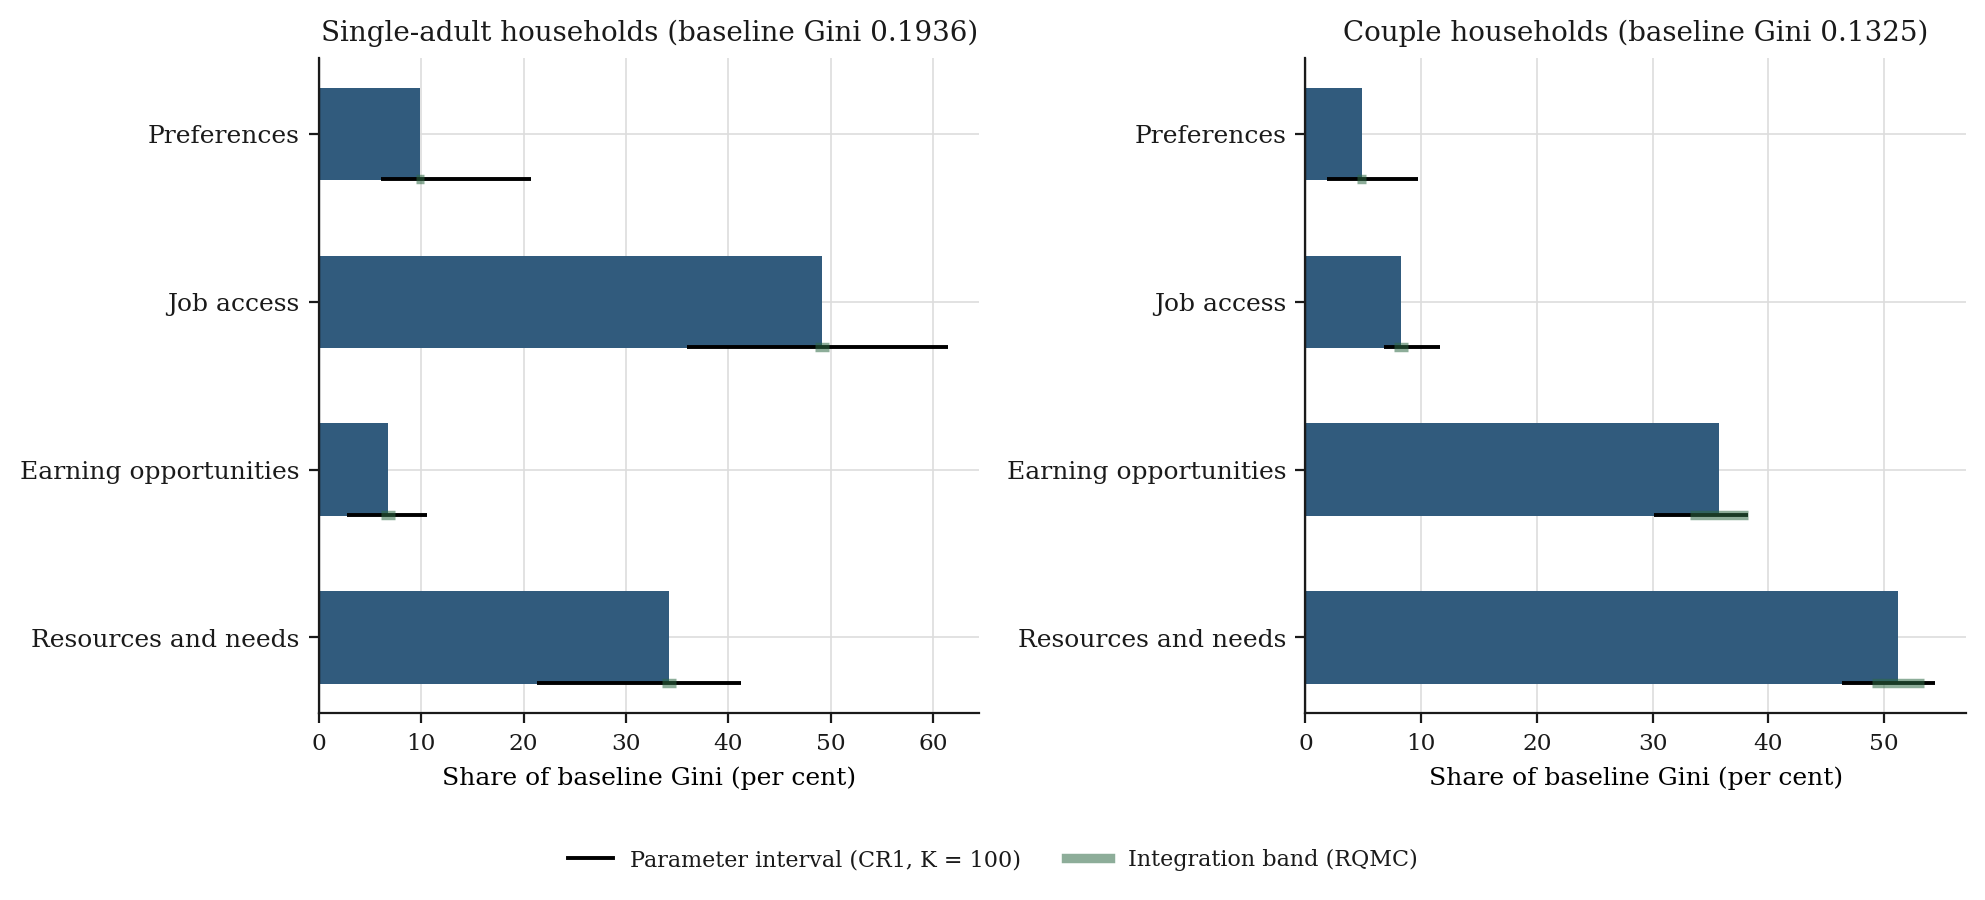
\includegraphics[width=0.95\linewidth,height=\textheight,keepaspectratio,alt={The grouped attribution, signed, in per cent of each population's own baseline Gini. The black bar is the 95 per cent cluster-robust parameter interval; the shaded bar is the RQMC integration band. They measure different things and are never combined.}]{figures/v5/figV03_signed_decomposition.png}
\caption{The grouped attribution, signed, in per cent of each population's own baseline Gini. The black bar is the 95 per cent cluster-robust parameter interval; the shaded bar is the RQMC integration band. They measure different things and are never combined.}
\end{figure}

The headline is the single-adult row. Labour-market opportunities, job access together with earning opportunities, carry 55.92 per cent of the inequality in the money metric; job access alone carries 49.16 per cent, with a 95 per cent cluster-robust parameter interval of 36.0 to 61.5 per cent. Preferences carry 9.88 per cent, earning opportunities 6.76 and household resources and needs 34.20. For couples the ordering is different: earning opportunities carry 35.72 per cent and resources and needs 51.20, while job access carries 8.23. Single adults are access-dominated on the labour-market side; couples are earnings- and resource-dominated, and access matters much less for them.

We report that contrast as a finding and attach no mechanism to it. A second earner is not automatically a buffer: two earnings streams do not mechanically produce less dispersion than one, since that depends on the dependence between them and on how resources pool. Establishing a mechanism would require a separately defined counterfactual, which we have not run. The contrast also cannot be assigned entirely to household type, because the two applications differ in their reference constructions as well; Section 6 reports the reference sensitivity.

The parameter interval and the integration band measure different things and are never combined. The integration band on the single-adult access share is 48.5 to 49.9 per cent, an order of magnitude narrower than the parameter interval, which is the expected ordering: the numerical integration is the accurate part and the parameters are the uncertain part.

The allocation is exhaustive. The maximum absolute top-level identity residual is 2.8e-17 in index units and the nested residual 5.6e-17. That is a computational validation of the accounting for the declared game. It does not validate the identification of the model or the normative content of the operators.


\subsection{Inside the budget channel: resources against composition and needs}\label{inside-the-budget-channel-resources-against-composition-and-needs}

The resources-and-needs contribution is itself two things: the non-labour resources a household has, and the size and composition of the household those resources must cover. Separating them is not an arithmetic split of the joint cell. It requires two further counterfactual panels, each repriced through the tax-benefit system, and it is done here on the corrected partition of the budget fields into 58 resource fields, 46 composition and needs fields and 6 geographic fields, which travel with resources.

\Needspace*{12\baselineskip}\small\setlength{\tabcolsep}{3pt}\begin{longtable}[]{@{}
  >{\raggedright\arraybackslash}p{(\linewidth - 12\tabcolsep) * \real{0.1429}}
  >{\raggedright\arraybackslash}p{(\linewidth - 12\tabcolsep) * \real{0.1429}}
  >{\raggedright\arraybackslash}p{(\linewidth - 12\tabcolsep) * \real{0.1429}}
  >{\raggedright\arraybackslash}p{(\linewidth - 12\tabcolsep) * \real{0.1429}}
  >{\raggedright\arraybackslash}p{(\linewidth - 12\tabcolsep) * \real{0.1429}}
  >{\raggedright\arraybackslash}p{(\linewidth - 12\tabcolsep) * \real{0.1429}}
  >{\raggedright\arraybackslash}p{(\linewidth - 12\tabcolsep) * \real{0.1429}}@{}}
\caption{The subdivision of the resources-and-needs contribution into non-labour resources and household composition and needs, reported as ``resources / composition'' in every cell. Columns two and five are shares of that population's baseline inequality; the remaining columns are shares of the resources-and-needs channel itself, which the two cells divide. The couple cells come from two counterfactual panels repriced through the tax-benefit system on the corrected partition of 58 resource fields, 46 composition and needs fields and 6 geographic fields, and sum to the joint contribution to a residual of 1.4e-17 in index units. The single-adult cells come from panels priced on an earlier partition of the same fields, so they are reported for comparison and the two populations' channel shares are indicative rather than like for like.}\tabularnewline
\toprule\noalign{}
\begin{minipage}[b]{\linewidth}\raggedright
Index
\end{minipage} & \begin{minipage}[b]{\linewidth}\raggedright
Couples: share of baseline
\end{minipage} & \begin{minipage}[b]{\linewidth}\raggedright
Couples: share of channel
\end{minipage} & \begin{minipage}[b]{\linewidth}\raggedright
Couples: channel, equivalized
\end{minipage} & \begin{minipage}[b]{\linewidth}\raggedright
Singles: share of baseline
\end{minipage} & \begin{minipage}[b]{\linewidth}\raggedright
Singles: share of channel
\end{minipage} & \begin{minipage}[b]{\linewidth}\raggedright
Singles: channel, equivalized
\end{minipage} \\
\midrule\noalign{}
\endfirsthead
\toprule\noalign{}
\begin{minipage}[b]{\linewidth}\raggedright
Index
\end{minipage} & \begin{minipage}[b]{\linewidth}\raggedright
Couples: share of baseline
\end{minipage} & \begin{minipage}[b]{\linewidth}\raggedright
Couples: share of channel
\end{minipage} & \begin{minipage}[b]{\linewidth}\raggedright
Couples: channel, equivalized
\end{minipage} & \begin{minipage}[b]{\linewidth}\raggedright
Singles: share of baseline
\end{minipage} & \begin{minipage}[b]{\linewidth}\raggedright
Singles: share of channel
\end{minipage} & \begin{minipage}[b]{\linewidth}\raggedright
Singles: channel, equivalized
\end{minipage} \\
\midrule\noalign{}
\endhead
\bottomrule\noalign{}
\endlastfoot
Gini & 32.88 / 18.33 & 64.2 / 35.8 & 57.1 / 42.9 & 24.38 / 9.82 & 71.3 / 28.7 & 46.1 / 53.9 \\
Atkinson(1) & 49.14 / 11.46 & 81.1 / 18.9 & 73.7 / 26.3 & 34.38 / 12.52 & 73.3 / 26.7 & 48.3 / 51.7 \\
Atkinson(2) & 44.42 / 12.79 & 77.6 / 22.4 & 68.3 / 31.7 & 31.33 / 12.24 & 71.9 / 28.1 & 44.2 / 55.8 \\
GE(0) & 49.15 / 11.42 & 81.2 / 18.8 & 73.8 / 26.2 & 34.62 / 12.57 & 73.4 / 26.6 & 48.4 / 51.6 \\
GE(1) & 55.49 / 9.44 & 85.5 / 14.5 & 80.4 / 19.6 & 39.26 / 13.47 & 74.4 / 25.6 & 53.4 / 46.6 \\
GE(2) \(=CV^2/2\) & 63.15 / 7.01 & 90.0 / 10.0 & 87.7 / 12.3 & 47.04 / 15.81 & 74.8 / 25.2 & 58.7 / 41.3 \\
\end{longtable}

Three statements are supported, and a fourth that suggests itself is not.

First, \textbf{non-labour resources lead the channel in both populations on the household basis, under all six indices} --- 6 of six for couples and 6 of six for single adults. On the Gini the couples channel divides 64.2 to 35.8, which is 32.88 and 18.33 per cent of total inequality; the single-adult channel divides 71.3 to 28.7, or 24.38 and 9.82 per cent of total.

Second, \textbf{the resources share of the channel is widest under GE(2) and narrowest under the Gini in both populations.} The Gini is the index least sensitive to the tails, and it is where composition matters most; the squared coefficient of variation is the most tail-sensitive, and it is where resources dominate. The spread is large --- for couples, from 64.2 per cent of the channel under the Gini to 90.0 under GE(2) --- so the division of this channel is considerably more index-sensitive than the four-way decomposition above it.

Third, \textbf{equivalizing raises the composition share in both populations, under all 6 of the six indices.} This is not an artefact and it is not a surprise: the equivalence scale is owned by the composition operator, so a state in which composition is equalized is also a state in which every household is put on a common scale. Equalizing composition therefore removes both the direct effect of household size on the budget and the effect of size on the scale by which the resulting level is deflated. For single adults the effect is strong enough to reverse the ordering: on the equivalized basis resources lead the channel in only 2 of the six indices, and composition leads under the Gini, both Atkinson indices and GE(0). For couples the ordering survives equivalization, under all 6 of the six.

The statement that does \emph{not} survive is a comparison between the two populations. On the Gini, composition takes a larger share of the couples channel than of the single-adult channel, 35.8 against 28.7 per cent, which invites the reading that household composition matters more where there is a household to compose. That ordering holds under 1 of the six indices, the Gini, and reverses under the other five; on the equivalized basis it reverses under all six. We therefore do not report it as a finding. The two populations' panels also rest on different partitions of the budget fields, which is a second reason to treat the cross-population comparison of channel shares as indicative.


\subsection{Index sensitivity}\label{index-sensitivity}

\Needspace*{12\baselineskip}\small\setlength{\tabcolsep}{3pt}\begin{longtable}[]{@{}
  >{\raggedright\arraybackslash}p{(\linewidth - 12\tabcolsep) * \real{0.1429}}
  >{\raggedright\arraybackslash}p{(\linewidth - 12\tabcolsep) * \real{0.1429}}
  >{\raggedright\arraybackslash}p{(\linewidth - 12\tabcolsep) * \real{0.1429}}
  >{\raggedright\arraybackslash}p{(\linewidth - 12\tabcolsep) * \real{0.1429}}
  >{\raggedright\arraybackslash}p{(\linewidth - 12\tabcolsep) * \real{0.1429}}
  >{\raggedright\arraybackslash}p{(\linewidth - 12\tabcolsep) * \real{0.1429}}
  >{\raggedright\arraybackslash}p{(\linewidth - 12\tabcolsep) * \real{0.1429}}@{}}
\caption{Baseline level and attribution shares under six inequality indices. Every row was recomputed for its own index against its own baseline; no coalition value or share is transferred between indices. Shares within a row sum to one hundred by exhaustiveness. A negative preference share means that equalizing preferences alone would raise that index, which is a property of this exhaustive two-group game with a nonnegative index and is explained in the text.}\tabularnewline
\toprule\noalign{}
\begin{minipage}[b]{\linewidth}\raggedright
Population and index
\end{minipage} & \begin{minipage}[b]{\linewidth}\raggedright
Baseline level
\end{minipage} & \begin{minipage}[b]{\linewidth}\raggedright
Preferences (per cent)
\end{minipage} & \begin{minipage}[b]{\linewidth}\raggedright
Access
\end{minipage} & \begin{minipage}[b]{\linewidth}\raggedright
Earning opportunities
\end{minipage} & \begin{minipage}[b]{\linewidth}\raggedright
Resources and needs
\end{minipage} & \begin{minipage}[b]{\linewidth}\raggedright
Access + earnings
\end{minipage} \\
\midrule\noalign{}
\endfirsthead
\toprule\noalign{}
\begin{minipage}[b]{\linewidth}\raggedright
Population and index
\end{minipage} & \begin{minipage}[b]{\linewidth}\raggedright
Baseline level
\end{minipage} & \begin{minipage}[b]{\linewidth}\raggedright
Preferences (per cent)
\end{minipage} & \begin{minipage}[b]{\linewidth}\raggedright
Access
\end{minipage} & \begin{minipage}[b]{\linewidth}\raggedright
Earning opportunities
\end{minipage} & \begin{minipage}[b]{\linewidth}\raggedright
Resources and needs
\end{minipage} & \begin{minipage}[b]{\linewidth}\raggedright
Access + earnings
\end{minipage} \\
\midrule\noalign{}
\endhead
\bottomrule\noalign{}
\endlastfoot
Single-adult, Gini & 0.193596 & 9.88 & 49.16 & 6.76 & 34.20 & 55.92 \\
Single-adult, Atkinson(1) & 0.060788 & -7.21 & 55.12 & 5.18 & 46.90 & 60.31 \\
Single-adult, Atkinson(2) & 0.115514 & -6.83 & 58.49 & 4.77 & 43.57 & 63.27 \\
Single-adult, GE(0) & 0.062714 & -7.86 & 55.42 & 5.26 & 47.19 & 60.67 \\
Single-adult, GE(1) & 0.065890 & -7.59 & 49.64 & 5.22 & 52.73 & 54.87 \\
Single-adult, GE(2) \(=CV^2/2\) & 0.153963 & -8.52 & 40.89 & 4.78 & 62.86 & 45.67 \\
Couple, Gini & 0.132465 & 4.85 & 8.23 & 35.72 & 51.20 & 43.95 \\
Couple, Atkinson(1) & 0.030197 & 2.52 & 6.38 & 30.50 & 60.60 & 36.88 \\
Couple, Atkinson(2) & 0.055239 & 2.74 & 6.94 & 33.10 & 57.21 & 40.05 \\
Couple, GE(0) & 0.030663 & 2.55 & 6.40 & 30.48 & 60.57 & 36.88 \\
Couple, GE(1) & 0.034637 & 2.27 & 5.70 & 27.09 & 64.94 & 32.79 \\
Couple, GE(2) \(=CV^2/2\) & 0.088142 & 2.03 & 4.95 & 22.87 & 70.16 & 27.82 \\
\end{longtable}

\begin{figure}[H]
\centering
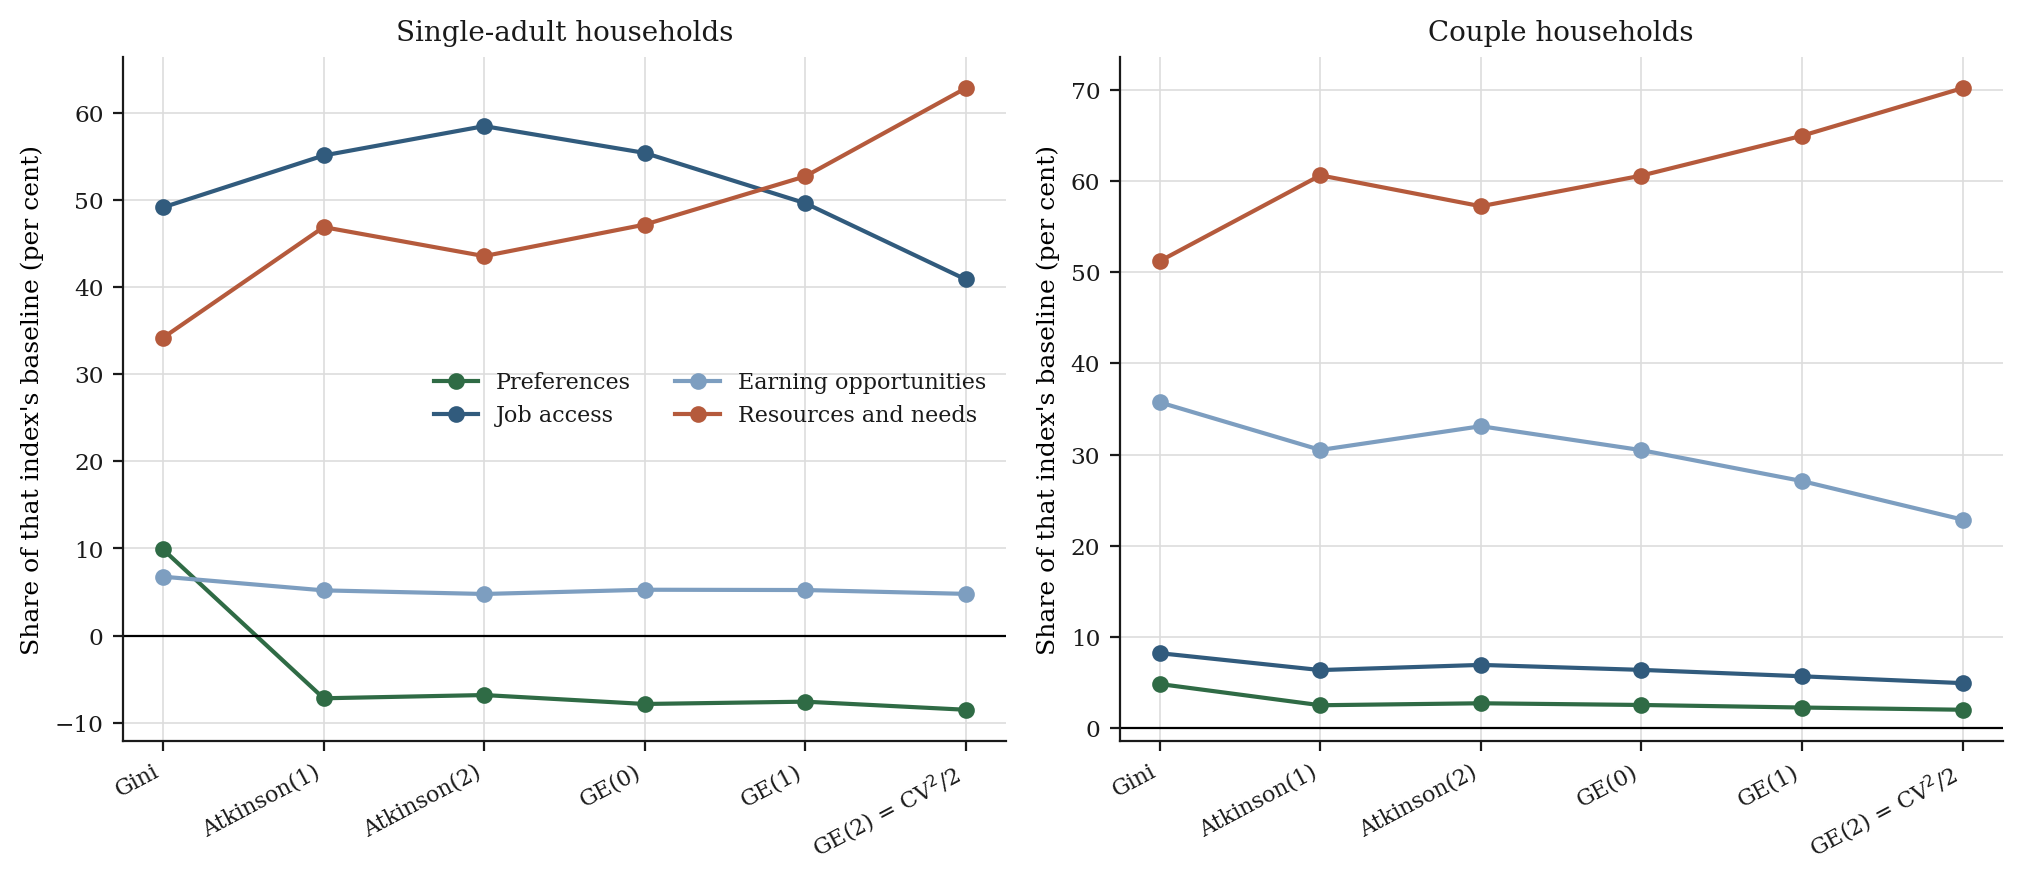
\includegraphics[width=0.95\linewidth,height=\textheight,keepaspectratio,alt={Attribution shares under six inequality indices. Each index keeps its own coalition values and its own allocation. Access exceeds earning opportunities for single adults under all six and the ordering reverses for couples under all six; the singles preference share changes sign outside the Gini.}]{figures/v5/figV05_six_index_shares.png}
\caption{Attribution shares under six inequality indices. Each index keeps its own coalition values and its own allocation. Access exceeds earning opportunities for single adults under all six and the ordering reverses for couples under all six; the singles preference share changes sign outside the Gini.}
\end{figure}

Each index keeps its own coalition values and its own allocation; nothing is transferred between rows. Read carefully, the table supports the following and not more.

\begin{itemize}
\tightlist
\item
  Job access exceeds earning opportunities for single adults under all 6 indices, and earning opportunities exceed access for couples under all 6. This is the robust ordering and it is the one we emphasise.
\item
  Job access alone exceeds resources and needs for single adults under 4 of the six; GE(1) and GE(2) are the exceptions.
\item
  Access and earning opportunities together exceed resources and needs for single adults under 5 of the six, with GE(2) the exception.
\item
  Resources and needs are the largest of the four components for couples under all 6 indices.
\item
  The single-adult preference share is positive for the Gini and negative under the other 5 indices. The preference contribution is therefore \emph{not} a metric-invariant conclusion, and the statement that preferences account for about ten per cent of inequality is a statement about the Gini on the raw basis under the female-primary reference, not a general one.
\end{itemize}

These are descriptive rankings of point estimates. Parameter intervals are reported for the Gini shares only, and we do not convert any of these orderings into a claim of statistical significance.


\section{Sensitivity and limitations}\label{sensitivity-and-limitations}

\subsection{The normative reference}\label{the-normative-reference}

The reference is a choice, and the results move with it. The single-adult decomposition uses a female-primary reference block; under the alternative male structural-zero reference the shares become 10.17 per cent for preferences, 51.55 for access, 7.56 for earning opportunities and 30.72 for resources and needs. The ordering is unchanged and the magnitudes move by a few percentage points. That sensitivity is real and belongs with the result; it is a property of the normative construction, not a numerical instability.

Equivalization is a second normative choice of the same kind. On the equivalized basis the single-adult access share falls and the resources-and-needs share rises, and the couples pattern moves in the same direction. Both bases are reported throughout; neither is the correct one, and the choice between them is not settled by the data.

\subsection{Two open econometric questions}\label{two-open-econometric-questions}

The sample screens on the observed hours and wage of employed deciders. The estimation sample is therefore selected on an outcome of the process being modelled, and the conditional sampled-set likelihood, which is the right object given a sampled choice set, is not automatically the right object given an outcome-selected sample. We have not established which correction the screen requires, or that none is required. This is an econometric question and not a presentational one, and it is not resolved by the diagnostics reported above.

Separately, the sampled-set probability is derived by conditioning on a labelled collection of slots. Small observed cross-coordinate correlations and a multiplicity distribution consistent with independent draws are diagnostics; they do not by themselves establish the sampling law that the derivation assumes. Both questions are recorded here as open.

\subsection{The bridge to the compensation-side reference}\label{the-bridge-to-the-compensation-side-reference}

The flat-consumption reference of Section 4 is one member of a family. A natural comparison is the reference that flattens consumption only at the non-work bundle, which sits on the compensation side of the same family. If non-work maximizes the non-consumption index and the opportunity density integrates to one on the domain the reference mass uses, then \(H_i\le e^{L_i(o)}\), so the gap \(\Delta_i=L_i(o)-\log H_i\) must be non-negative for every household and the ratio of the two measures is bounded on one side.

The first premise holds for every household in both samples. The second does not: the opportunity object entering the reference mass is an unnormalized index whose median mass on that domain is 0.077283 for single adults and 147.963 for couples. Omitting that mass makes the comparison depend on an arbitrary multiplicative scale, and it is the reason earlier signed gaps had the wrong sign for couples and happened not to reverse for single adults. Both earlier levels are withdrawn.

\Needspace*{12\baselineskip}\small\setlength{\tabcolsep}{3pt}\begin{longtable}[]{@{}
  >{\raggedright\arraybackslash}p{(\linewidth - 12\tabcolsep) * \real{0.1429}}
  >{\raggedright\arraybackslash}p{(\linewidth - 12\tabcolsep) * \real{0.1429}}
  >{\raggedright\arraybackslash}p{(\linewidth - 12\tabcolsep) * \real{0.1429}}
  >{\raggedright\arraybackslash}p{(\linewidth - 12\tabcolsep) * \real{0.1429}}
  >{\raggedright\arraybackslash}p{(\linewidth - 12\tabcolsep) * \real{0.1429}}
  >{\raggedright\arraybackslash}p{(\linewidth - 12\tabcolsep) * \real{0.1429}}
  >{\raggedright\arraybackslash}p{(\linewidth - 12\tabcolsep) * \real{0.1429}}@{}}
\caption{The bridge between the two monetary references, after the premise audit. The second column reports whether non-work maximizes the non-consumption index for every household; the third reports the median mass of the opportunity kernel on the domain the reference integral uses. That mass is not one, which is the premise that failed and the reason the earlier signed gaps were scale artefacts. The remaining columns are the bridge after normalizing the kernel on exactly that domain.}\tabularnewline
\toprule\noalign{}
\begin{minipage}[b]{\linewidth}\raggedright
Population
\end{minipage} & \begin{minipage}[b]{\linewidth}\raggedright
Non-work maximizes \(L\)
\end{minipage} & \begin{minipage}[b]{\linewidth}\raggedright
Median \(\int\hat g\)
\end{minipage} & \begin{minipage}[b]{\linewidth}\raggedright
Median \(W^4/W^1\)
\end{minipage} & \begin{minipage}[b]{\linewidth}\raggedright
Range
\end{minipage} & \begin{minipage}[b]{\linewidth}\raggedright
Median \(\Delta\) (nats)
\end{minipage} & \begin{minipage}[b]{\linewidth}\raggedright
\(\Delta\ge 0\) everywhere
\end{minipage} \\
\midrule\noalign{}
\endfirsthead
\toprule\noalign{}
\begin{minipage}[b]{\linewidth}\raggedright
Population
\end{minipage} & \begin{minipage}[b]{\linewidth}\raggedright
Non-work maximizes \(L\)
\end{minipage} & \begin{minipage}[b]{\linewidth}\raggedright
Median \(\int\hat g\)
\end{minipage} & \begin{minipage}[b]{\linewidth}\raggedright
Median \(W^4/W^1\)
\end{minipage} & \begin{minipage}[b]{\linewidth}\raggedright
Range
\end{minipage} & \begin{minipage}[b]{\linewidth}\raggedright
Median \(\Delta\) (nats)
\end{minipage} & \begin{minipage}[b]{\linewidth}\raggedright
\(\Delta\ge 0\) everywhere
\end{minipage} \\
\midrule\noalign{}
\endhead
\bottomrule\noalign{}
\endlastfoot
Single-adult & yes & 0.077283 & 0.9843 & {[}0.9169, 0.9990{]} & 0.0322 & yes \\
Couple & yes & 147.962795 & 0.6242 & {[}0.5211, 0.7171{]} & 0.9906 & yes \\
\end{longtable}

After normalizing the kernel on exactly the domain the reference mass uses, the bridge is well behaved: the gap is non-negative for every household in both samples and the ratio is at most one everywhere, as the premises require. The median ratio is 0.9843 for single adults and 0.6242 for couples. We report the reconciled bridge as a property comparison between two references and do not use it as a competing headline distribution.

\subsection{The relative-index companion measure}\label{the-relative-index-companion-measure}

A third reference, which flattens the sum of a resource base and gross pay rather than disposable consumption, is defined only where the inversion brackets. It brackets for all 1,540 single-adult households with no negative values, and is therefore usable as a single-adult diagnostic. For couples it brackets for 9 of 2,223 households in the theory-strict form, and the household-resource form produces 2,103 negative values, on which relative inequality indices are not defined. We therefore treat it as a single-adult diagnostic and do not force it into the couples application. Failure to bracket is not by itself proof that a measure does not exist; here the three cases we can distinguish are an insufficient upper bracket, an empty positive-consumption domain and a target below the attainable reference range, and we report which applies rather than a single count.

\subsection{The consumption normalizer}\label{the-consumption-normalizer}

\Needspace*{12\baselineskip}\small\setlength{\tabcolsep}{3pt}\begin{longtable}[]{@{}
  >{\raggedright\arraybackslash}p{(\linewidth - 6\tabcolsep) * \real{0.2500}}
  >{\raggedright\arraybackslash}p{(\linewidth - 6\tabcolsep) * \real{0.2500}}
  >{\raggedright\arraybackslash}p{(\linewidth - 6\tabcolsep) * \real{0.2500}}
  >{\raggedright\arraybackslash}p{(\linewidth - 6\tabcolsep) * \real{0.2500}}@{}}
\caption{The consumption normalizer. Three constants were in circulation. Under exact log consumption the normalizer enters utility as the alternative-invariant term \(-\beta_c\log\lambda_c\), so it cancels from every choice probability and exactly from the money metric. The paper reports the estimation-frame constant throughout.}\tabularnewline
\toprule\noalign{}
\begin{minipage}[b]{\linewidth}\raggedright
Panel
\end{minipage} & \begin{minipage}[b]{\linewidth}\raggedright
Single-adult (EUR/month)
\end{minipage} & \begin{minipage}[b]{\linewidth}\raggedright
Couple (EUR/month)
\end{minipage} & \begin{minipage}[b]{\linewidth}\raggedright
Role
\end{minipage} \\
\midrule\noalign{}
\endfirsthead
\toprule\noalign{}
\begin{minipage}[b]{\linewidth}\raggedright
Panel
\end{minipage} & \begin{minipage}[b]{\linewidth}\raggedright
Single-adult (EUR/month)
\end{minipage} & \begin{minipage}[b]{\linewidth}\raggedright
Couple (EUR/month)
\end{minipage} & \begin{minipage}[b]{\linewidth}\raggedright
Role
\end{minipage} \\
\midrule\noalign{}
\endhead
\bottomrule\noalign{}
\endlastfoot
Estimation frame, 101 sampled alternatives per household & 1,938.238719 & 4,247.875047 & Constant of record \\
Welfare panel, 2,048 common integration nodes & 1,774.518218 & 3,821.448012 & Recomputed over its own rows; inert \\
Predecessor frames, before the sample correction & 1,911.108058 & 3,821.448012 & Superseded \\
\end{longtable}

Three normalizing constants were in circulation between the estimation frames and the welfare panel, because each panel computes the constant as a mean over its own rows. Under exact log consumption the constant is alternative-invariant, so it cancels from every choice probability and exactly from the money metric; the deviation over four widely separated values is 2.7e-15. No reported quantity changes. The paper reports the estimation-frame constant throughout, and the discrepancy is recorded here rather than silently harmonised.

\subsection{What is not established}\label{what-is-not-established}

The decomposition is an accounting of a structural model under declared operators. It is not a causal analysis. No regional, educational or occupational effect reported here is identified as a causal effect, and the exhaustiveness of the allocation validates the accounting for the declared game, not the identification of the model or the normative content of the operators.

The parameter intervals cover the Gini shares; the other five indices are reported as point estimates. The subdivision of the couples resources-and-needs component reported in Section 5 rests on two counterfactual panels repriced through the tax-benefit system rather than on any imputation, but it is a nested result within the joint component and the joint component remains what the headline decomposition reports. The corresponding subdivision for single adults is \emph{not} reported: the only priced panels available for it encode an earlier partition of the budget fields, so its two cells are not comparable with the couples cells and are not a current result.


\section{Conclusion}\label{conclusion}

Observed hours and earnings do not say whether a household chose its position or settled for it, and that ambiguity is not a nuisance for welfare measurement: it is the substance of it. This paper takes the ambiguity seriously in both halves of the problem. On the behavioural side it estimates a model in which the jobs a household can reach and the way it ranks them are identified jointly, with every alternative priced through the tax-benefit system. On the normative side it evaluates well-being with a reference that keeps each household's own preferences and own reachable jobs and removes variation in pay from the reference bundles.

The decomposition then asks how the resulting inequality divides. For French single-adult households, labour-market opportunities carry 55.92 per cent of it and job access alone 49.16 per cent, more than household resources and needs and far more than preferences. For couples the same accounting gives a different answer: earning opportunities and household circumstances dominate and access matters little. The ordering of access against earnings within each type is the part that survives all six inequality indices we report; the preference contribution is not, and changes sign outside the Gini.

Three limits should travel with those numbers. The measure is one member of a family of references and the shares move with the reference, in ways we report rather than resolve. The allocation is exhaustive for the declared game, which validates the accounting and not the identification or the ethics of the operators. And two questions about the observation rule remain genuinely open. What the exercise offers is not a causal account of why opportunities differ, but a disciplined statement of how much of measured well-being inequality is associated with them once preferences, resources and needs are modelled explicitly and the reference is stated.


\appendix

\section{Appendix A. The estimated parameter vectors}\label{appendix-a.-the-estimated-parameter-vectors}

The tables below report only coordinates estimated on the reported sample. \textbf{Maintained restrictions.} Singles: \texttt{theta\_c\_singles\ =\ 0}; the couples preference block (\texttt{beta\_l0\_m}, \texttt{beta\_l\_age\_m}, \texttt{beta\_l\_age2\_m}, \texttt{beta\_l0\_f}, \texttt{beta\_l\_age\_f}, \texttt{beta\_l\_age2\_f}, \texttt{beta\_l\_nkids\_f}, \texttt{theta\_l\_f}) does not enter the singles likelihood; and \texttt{beta\_E\_y2015} and \texttt{beta\_E\_y2017} are absent because the 2015 and 2017 data are not used. Couples: \texttt{theta\_c\ =\ 0}, the male children leisure effect is structurally zero, and the direct cross-leisure term is fixed at zero. These are restrictions, not estimates.

One single-adult coordinate, the female age-square term, is at its box endpoint. Under the active-set convention its interval is not reported, the interior curvature is computed after removing it, and the parameter draws used for the welfare intervals hold it at its estimate.

\Needspace*{12\baselineskip}\small\setlength{\tabcolsep}{3pt}\begin{longtable}[]{@{}>{\RaggedRight\arraybackslash}p{0.2500\linewidth}>{\RaggedRight\arraybackslash}p{0.1292\linewidth}>{\RaggedRight\arraybackslash}p{0.1292\linewidth}>{\RaggedRight\arraybackslash}p{0.1292\linewidth}>{\RaggedRight\arraybackslash}p{0.1292\linewidth}>{\RaggedRight\arraybackslash}p{0.1292\linewidth}@{}}
\caption{The singles estimated coordinates. Standard errors are cluster-robust on the household; boundary-active estimates are marked at bound. Maintained restrictions are stated once in the accompanying note.}\tabularnewline
\toprule\noalign{}
Coordinate & Estimate & CR1 s.e. & z & Box & Status \\
\midrule\noalign{}
\endfirsthead
\toprule\noalign{}
Coordinate & Estimate & CR1 s.e. & z & Box & Status \\
\midrule\noalign{}
\endhead
\bottomrule\noalign{}
\endlastfoot
\path{beta_l0_sm} & 8.51993 & 3.54798 & 2.401 & {[}0.05, 50{]} & estimated \\
\path{beta_l_age_sm} & 1.48195 & 1.02361 & 1.448 & {[}-5, 5{]} & estimated \\
\path{beta_l_age2_sm} & 0.778284 & 0.773158 & 1.007 & {[}-1, 1{]} & estimated \\
\path{theta_l_sm} & -1.62627 & 0.330058 & -4.927 & {[}-8, 0.95{]} & estimated \\
\path{beta_l0_sf} & 5.86829 & 2.13459 & 2.749 & {[}0.05, 50{]} & estimated \\
\path{beta_l_age_sf} & 0.0677662 & 0.479217 & 0.141 & {[}-5, 5{]} & estimated \\
\path{beta_l_age2_sf} & 1 & -- & -- & {[}-1, 1{]} & at bound \\
\path{beta_l_nkids_sf} & 0.166636 & 0.442236 & 0.377 & {[}-5, 5{]} & estimated \\
\path{theta_l_sf} & -0.927353 & 0.216128 & -4.291 & {[}-8, 0.95{]} & estimated \\
\path{beta_E} & -3.17353 & 0.405337 & -7.829 & {[}-25, 25{]} & estimated \\
\path{beta_h_pt1} & 0.0297672 & 0.197247 & 0.151 & {[}-10, 10{]} & estimated \\
\path{beta_h_pt2} & 0.707971 & 0.192788 & 3.672 & {[}-10, 10{]} & estimated \\
\path{beta_h_ft} & 1.93873 & 0.0996968 & 19.446 & {[}-10, 10{]} & estimated \\
\path{beta_h_lh} & -0.0833752 & 0.177201 & -0.471 & {[}-10, 10{]} & estimated \\
\path{beta_E_gsur} & -1.44224 & 0.235591 & -6.122 & {[}-10, 10{]} & estimated \\
\path{beta_E_drgn2} & -0.377963 & 0.32925 & -1.148 & {[}-10, 10{]} & estimated \\
\path{beta_E_drgn3} & -0.111713 & 0.38912 & -0.287 & {[}-10, 10{]} & estimated \\
\path{beta_E_drgn4} & -0.821813 & 0.380963 & -2.157 & {[}-10, 10{]} & estimated \\
\path{beta_E_drgn5} & -0.516158 & 0.327362 & -1.577 & {[}-10, 10{]} & estimated \\
\path{beta_E_drgn6} & -0.722159 & 0.35278 & -2.047 & {[}-10, 10{]} & estimated \\
\path{beta_E_drgn7} & -0.537369 & 0.350308 & -1.534 & {[}-10, 10{]} & estimated \\
\path{beta_E_drgn8} & -0.45119 & 0.340074 & -1.327 & {[}-10, 10{]} & estimated \\
\path{beta_E_drgur} & -0.0287689 & 0.220916 & -0.130 & {[}-10, 10{]} & estimated \\
\path{beta_E_drgmd} & 0.064133 & 0.261352 & 0.245 & {[}-10, 10{]} & estimated \\
\path{beta_occ_2_m} & -1.37371 & 0.158147 & -8.686 & {[}-15, 15{]} & estimated \\
\path{beta_occ_3_m} & -2.10963 & 0.202248 & -10.431 & {[}-15, 15{]} & estimated \\
\path{beta_occ_4_m} & -0.325897 & 0.121341 & -2.686 & {[}-15, 15{]} & estimated \\
\path{beta_occ_2_f} & 0.113492 & 0.137399 & 0.826 & {[}-15, 15{]} & estimated \\
\path{beta_occ_3_f} & -0.406009 & 0.144045 & -2.819 & {[}-15, 15{]} & estimated \\
\path{beta_occ_4_f} & 0.563216 & 0.122467 & 4.599 & {[}-15, 15{]} & estimated \\
\path{beta_w0} & 2.01382 & 0.0560922 & 35.902 & {[}-10, 20{]} & estimated \\
\path{beta_w_educL} & 0.0566261 & 0.0372485 & 1.520 & {[}-5, 5{]} & estimated \\
\path{beta_w_educH} & 0.149054 & 0.0308408 & 4.833 & {[}-5, 5{]} & estimated \\
\path{beta_w_pexp} & 0.24077 & 0.0862223 & 2.792 & {[}-1, 1{]} & estimated \\
\path{beta_w_pexp2} & -0.0281739 & 0.0389905 & -0.723 & {[}-0.1, 0.1{]} & estimated \\
\path{sigma} & 0.381505 & 0.0132752 & 28.738 & {[}0.1, 20{]} & estimated \\
\path{delta_occ_2} & -0.0347155 & 0.039899 & -0.870 & {[}-4, 4{]} & estimated \\
\path{delta_occ_3} & 0.0622139 & 0.0382749 & 1.625 & {[}-4, 4{]} & estimated \\
\path{delta_occ_4} & 0.278494 & 0.0367705 & 7.574 & {[}-4, 4{]} & estimated \\
\path{beta_h_f35} & 2.06556 & 0.0894479 & 23.092 & {[}-10, 10{]} & estimated \\
\path{beta_c} & 2.03873 & 0.291729 & 6.988 & {[}0.05, 50{]} & estimated \\
\end{longtable}

\Needspace*{12\baselineskip}\small\setlength{\tabcolsep}{3pt}\begin{longtable}[]{@{}>{\RaggedRight\arraybackslash}p{0.2500\linewidth}>{\RaggedRight\arraybackslash}p{0.1292\linewidth}>{\RaggedRight\arraybackslash}p{0.1292\linewidth}>{\RaggedRight\arraybackslash}p{0.1292\linewidth}>{\RaggedRight\arraybackslash}p{0.1292\linewidth}>{\RaggedRight\arraybackslash}p{0.1292\linewidth}@{}}
\caption{The couples estimated coordinates. Standard errors are cluster-robust on the household; boundary-active estimates are marked at bound. Maintained restrictions are stated once in the accompanying note.}\tabularnewline
\toprule\noalign{}
Coordinate & Estimate & CR1 s.e. & z & Box & Status \\
\midrule\noalign{}
\endfirsthead
\toprule\noalign{}
Coordinate & Estimate & CR1 s.e. & z & Box & Status \\
\midrule\noalign{}
\endhead
\bottomrule\noalign{}
\endlastfoot
\path{beta_l0_m} & 3.98136 & 0.746569 & 5.333 & {[}1e-06, 50{]} & estimated \\
\path{beta_l_age_m} & -0.00799228 & 0.0287174 & -0.278 & {[}-5, 5{]} & estimated \\
\path{beta_l_age2_m} & 0.00648336 & 0.00297388 & 2.180 & {[}-1, 1{]} & estimated \\
\path{theta_l_m} & -0.976109 & 0.135663 & -7.195 & {[}-8, 0.95{]} & estimated \\
\path{beta_l0_f} & 13.1029 & 4.77604 & 2.743 & {[}0.05, 50{]} & estimated \\
\path{beta_l_age_f} & -0.122813 & 0.126048 & -0.974 & {[}-5, 5{]} & estimated \\
\path{beta_l_age2_f} & 0.00730709 & 0.0102503 & 0.713 & {[}-1, 1{]} & estimated \\
\path{beta_l_nkids_f} & -0.305471 & 1.14719 & -0.266 & {[}-5, 5{]} & estimated \\
\path{theta_l_f} & -1.68631 & 0.245846 & -6.859 & {[}-8, 0.95{]} & estimated \\
\path{beta_E_m} & -2.12326 & 0.319457 & -6.646 & {[}-25, 25{]} & estimated \\
\path{beta_E_f} & -2.81476 & 0.302078 & -9.318 & {[}-25, 25{]} & estimated \\
\path{beta_h_pt1_m} & -1.10936 & 0.379086 & -2.926 & {[}-10, 10{]} & estimated \\
\path{beta_h_pt1_f} & -0.517276 & 0.162932 & -3.175 & {[}-10, 10{]} & estimated \\
\path{beta_h_pt2_m} & 0.0835202 & 0.237788 & 0.351 & {[}-10, 10{]} & estimated \\
\path{beta_h_pt2_f} & 1.15858 & 0.121438 & 9.541 & {[}-10, 10{]} & estimated \\
\path{beta_h_f35_m} & 2.2888 & 0.0821348 & 27.866 & {[}-10, 10{]} & estimated \\
\path{beta_h_f35_f} & 2.02835 & 0.0682392 & 29.724 & {[}-10, 10{]} & estimated \\
\path{beta_h_ft_m} & 2.38012 & 0.0865569 & 27.498 & {[}-10, 10{]} & estimated \\
\path{beta_h_ft_f} & 1.68251 & 0.0798241 & 21.078 & {[}-10, 10{]} & estimated \\
\path{beta_h_lh_m} & 0.69767 & 0.133487 & 5.226 & {[}-10, 10{]} & estimated \\
\path{beta_h_lh_f} & -0.310873 & 0.161533 & -1.925 & {[}-10, 10{]} & estimated \\
\path{beta_E_gsur} & -1.19243 & 0.155667 & -7.660 & {[}-10, 10{]} & estimated \\
\path{beta_E_drgn2} & -0.154617 & 0.24423 & -0.633 & {[}-10, 10{]} & estimated \\
\path{beta_E_drgn3} & 0.0872501 & 0.280833 & 0.311 & {[}-10, 10{]} & estimated \\
\path{beta_E_drgn4} & 0.0150136 & 0.306753 & 0.049 & {[}-10, 10{]} & estimated \\
\path{beta_E_drgn5} & -0.145472 & 0.255453 & -0.569 & {[}-10, 10{]} & estimated \\
\path{beta_E_drgn6} & -0.284391 & 0.274814 & -1.035 & {[}-10, 10{]} & estimated \\
\path{beta_E_drgn7} & -0.139569 & 0.265133 & -0.526 & {[}-10, 10{]} & estimated \\
\path{beta_E_drgn8} & -0.165927 & 0.26603 & -0.624 & {[}-10, 10{]} & estimated \\
\path{beta_E_drgur} & -0.182322 & 0.165665 & -1.101 & {[}-10, 10{]} & estimated \\
\path{beta_E_drgmd} & -0.417356 & 0.1861 & -2.243 & {[}-10, 10{]} & estimated \\
\path{beta_occ_2_m} & -1.50975 & 0.0967347 & -15.607 & {[}-15, 15{]} & estimated \\
\path{beta_occ_3_m} & -2.25319 & 0.124405 & -18.112 & {[}-15, 15{]} & estimated \\
\path{beta_occ_4_m} & 0.159368 & 0.061796 & 2.579 & {[}-15, 15{]} & estimated \\
\path{beta_occ_2_f} & 0.207379 & 0.0891054 & 2.327 & {[}-15, 15{]} & estimated \\
\path{beta_occ_3_f} & -0.180381 & 0.0923137 & -1.954 & {[}-15, 15{]} & estimated \\
\path{beta_occ_4_f} & 0.81589 & 0.079925 & 10.208 & {[}-15, 15{]} & estimated \\
\path{beta_w0} & 2.048 & 0.0335421 & 61.058 & {[}-10, 20{]} & estimated \\
\path{beta_w_educL} & -0.0433046 & 0.0216643 & -1.999 & {[}-5, 5{]} & estimated \\
\path{beta_w_educH} & 0.181652 & 0.0197059 & 9.218 & {[}-5, 5{]} & estimated \\
\path{beta_w_pexp} & 0.56435 & 0.0545928 & 10.337 & {[}-3, 3{]} & estimated \\
\path{beta_w_pexp2} & -0.15983 & 0.0242888 & -6.580 & {[}-0.3, 0.3{]} & estimated \\
\path{sigma} & 0.363075 & 0.0072235 & 50.263 & {[}0.1, 20{]} & estimated \\
\path{delta_occ_2} & -0.0740322 & 0.0231318 & -3.200 & {[}-4, 4{]} & estimated \\
\path{delta_occ_3} & 0.0393566 & 0.0228 & 1.726 & {[}-4, 4{]} & estimated \\
\path{delta_occ_4} & 0.214559 & 0.0223344 & 9.607 & {[}-4, 4{]} & estimated \\
\path{beta_c} & 2.10172 & 0.293879 & 7.152 & {[}0.05, 50{]} & estimated \\
\end{longtable}


\section{Appendix B. Inequality indices and the allocation rule}\label{appendix-b.-inequality-indices-and-the-allocation-rule}

\Needspace*{12\baselineskip}\small\setlength{\tabcolsep}{3pt}\begin{longtable}[]{@{}
  >{\raggedright\arraybackslash}p{(\linewidth - 2\tabcolsep) * \real{0.5000}}
  >{\raggedright\arraybackslash}p{(\linewidth - 2\tabcolsep) * \real{0.5000}}@{}}
\caption{The six inequality indices, defined on a weighted distribution of strictly positive levels with mean \(\mu\). Multiplying an index by a positive constant scales its level and its contributions but not its shares, so GE(2) and the squared coefficient of variation are the same game. Atkinson(1) and GE(0) rank any positive distribution identically because \(A(1)=1-e^{-GE(0)}\); their shares can nevertheless differ, because a nonlinear transformation does not commute with averaging marginal contributions over coalition orders.}\tabularnewline
\toprule\noalign{}
\begin{minipage}[b]{\linewidth}\raggedright
Index
\end{minipage} & \begin{minipage}[b]{\linewidth}\raggedright
Definition
\end{minipage} \\
\midrule\noalign{}
\endfirsthead
\toprule\noalign{}
\begin{minipage}[b]{\linewidth}\raggedright
Index
\end{minipage} & \begin{minipage}[b]{\linewidth}\raggedright
Definition
\end{minipage} \\
\midrule\noalign{}
\endhead
\bottomrule\noalign{}
\endlastfoot
Gini & \(\frac{1}{2\mu}\,\mathbb{E}\lvert W-\tilde W\rvert\), for \(W,\tilde W\) independent draws from the distribution \\
Atkinson(1) & \(1-\exp\!\big(\mathbb{E}\log W\big)/\mu\) \\
Atkinson(2) & \(1-\big(\mathbb{E}[W^{-1}]\big)^{-1}/\mu\) \\
GE(0) & \(\mathbb{E}\log(\mu/W)\) \\
GE(1) & \(\mathbb{E}\big[(W/\mu)\log(W/\mu)\big]\) \\
GE(2) \(=CV^2/2\) & \(\tfrac{1}{2}\mathbb{E}\big[(W/\mu)^2-1\big]\) \\
\end{longtable}

Two relations are worth stating because they explain apparent puzzles in the six-index table. First, multiplying an index by a positive constant scales its level and every contribution but leaves the shares unchanged, so GE(2) and the squared coefficient of variation define the same allocation game and are not two robustness checks. Second, \(A(1)=1-e^{-GE(0)}\), so Atkinson(1) and GE(0) rank any distribution of positive levels identically. Their allocated shares can nevertheless differ, because a nonlinear transformation of the index does not commute with averaging marginal contributions over coalition orders. That is a property of the allocation rule, not an inconsistency.

The Owen value for the partition \(\{\{P\},\{A,B,D\}\}\) allocates first between the two unions and then within the second, averaging over the orders of unions and, within a union, over the orders of its members. Contributions are signed and are never renormalised to sum to one hundred by construction: they sum to \(I_\varnothing-I_{\{P,A,B,D\}}\) because the game closes, and the closure is verified.


\section{Appendix C. The bridge between the two monetary references}\label{appendix-c.-the-bridge-between-the-two-monetary-references}

Write \(M_i=\int\widehat g_i\,d\nu\) for the mass of the opportunity object on the domain the reference integral uses, and \(o\) for the non-work bundle. The two references satisfy

\[
\beta_c\log(W^{1}_i/\lambda_c)=\log J_i-\log H_i,
\qquad
\beta_c\log(W^{4}_i/\lambda_c)=\log J_i-\log M_i-L_i(o),
\]

so that \(\log(W^{4}_i/W^{1}_i)=\big(\log H_i-\log M_i-L_i(o)\big)/\beta_c\) and \(\Delta_i=L_i(o)+\log M_i-\log H_i\). Omitting \(\log M_i\) is valid only when \(M_i=1\), and it is not: the audit reports median mass 0.077283 for single adults and 147.963 for couples. The premise that failed is therefore the unit mass of the kernel on that domain, not the maximality of the non-work bundle, which holds for every household in both samples, and not the orientation of the comparison.

After renormalizing the kernel on exactly that domain, the median gap is 0.0322 nats for single adults and 0.9906 for couples, the gap is non-negative for every household, and the ratio lies in \([0.9169, 0.9990]\) for single adults and \([0.5211, 0.7171]\) for couples. The identity above is satisfied to machine precision at the corrected normalization.

A separate point concerns the low-temperature limit. Attained and reference values must be indexed by the same shock scale for the limit to be meaningful. The statement that survives is that the two consistently indexed measures converge as the scale goes to zero; convergence to the value of staying at home evaluated at a different fixed scale is not the same statement and is not made.


\section{Appendix D. Data, software and replication}\label{appendix-d.-data-software-and-replication}

\textbf{Data.} French EU-SILC, accessed through Eurostat's harmonised release, with 2016 survey collection and a 2015 income reference year. The harmonised survey is transformed into an input file for EUROMOD \citep{sutherlandfigari2013}, which applies the French 2015 policy system. Regional labour-market conditions come from the Eurostat regional labour-force series. Access to EU-SILC microdata is granted by Eurostat under its research-access conditions and the data cannot be redistributed with this document.

\textbf{Sample.} 1,540 single-adult and 2,223 couple households, constructed by the screens of Section 2.

\textbf{Estimator and inference.} Conditional likelihood over 100 sampled alternatives per household plus the observed choice, with an out-of-fold proposal correction; cluster-robust standard errors on the household. Optimization is checked by five starts under two polishing contracts and curvature by exact Hessian eigenvalues.

\textbf{Welfare computation.} A common integration panel of 2,048 nodes per household, evaluated under all sixteen coalition states. Integration error is measured by 8 randomized quasi-Monte Carlo scrambles; parameter uncertainty by 100 draws from the cluster-robust covariance rebuilt from the Hessian and the household scores, holding maintained restrictions and bound-active coordinates at their values. The two are reported separately and are never combined into one band.

\textbf{Software.} Python with JAX (0.10.1) for automatic differentiation, and the EUROMOD connector (0.2.17).

\textbf{Replication.} Code and derived, non-confidential intermediate artefacts will be made available in a public repository on publication. Confidential microdata remain in their permitted environment, so the replication package reproduces every step conditional on authorised access to EU-SILC.


\section{Scientific history of this result}\label{scientific-history-of-this-result}

This section records how the reported specifications and results came to be what they are. It is here so that the argument above does not have to carry it, and so that a reader comparing this version with an earlier one can see what changed and why. Nothing in it is a competing model.

\textbf{The consumption specification.} Earlier drafts reported a specification in which the consumption coefficient was fixed at one as a numeraire, and one in which the single-adult consumption curvature was estimated at \(\theta_c\approx0.168\). Neither is the reported model. The current specification fixes the shock scale, fixes the consumption curvature at exactly zero, and estimates the consumption weight instead. That change improves the criterion by 23.753 log-points for single adults and 15.659 for couples, and it changes the welfare aggregator from an arithmetic mean of reachable consumption to a power mean of order \(\beta_c\). Every welfare quantity computed under the earlier convention is superseded, and the corresponding figures were regenerated rather than relabelled.

\textbf{The sample.} The predecessor frames contained 1,555 single-adult and 2,275 couple households. Twelve single-adult and fifty-two couple households were removed when the hours support and the occupation mapping were applied to the observed rows, and three further single-adult households were removed because their own observed job prices to non-positive disposable consumption. The current descriptive tables are computed on the resulting 1,540 and 2,223 households, not on the predecessor frames, and the funnel in Section 2 ends where the estimation begins.

\textbf{The disposable-income convention.} Single-adult disposable income was previously aggregated over the decider only; it is now aggregated over all resident household members, which is the convention the couples application always used. The two applications are now on the same accounting convention.

\textbf{The decomposition result.} An earlier draft reported household endowments and needs as the largest component for single adults, and a one-factor figure of about seventy-seven per cent. Both are withdrawn. The corrected computation gives 49.16 per cent to job access against 34.20 to resources and needs, and the corresponding one-factor effect for all non-preference circumstances is 67.2 per cent.

\textbf{The bridge between references.} The signed gap between the flat-consumption reference and the non-work-bundle reference was previously reported with the wrong sign for couples. The premise audit in Section 6 locates the cause in the normalization of the opportunity kernel on the domain the reference mass uses, and the corrected bridge satisfies the inequality the premises require in both samples.

\textbf{The consumption normalizer.} Three values of \(\lambda_c\) were in circulation because different panels recomputed it over their own rows. Under exact log consumption the constant cancels from the money metric, so no result changed; the paper now reports one constant per population.


\bibliographystyle{plainnat}
\bibliography{JMP_working_paper_for_seminar_v5}
\end{document}
